\chapter{Error Sources Affecting Relative Quantification of CEUS}
\label{chapter:PLOSONE}

% \section{Abstract}
% Lorem ipsum dolor sit amet, consectetur adipiscing elit. Curabitur eget porta erat. Morbi consectetur est vel gravida pretium. Suspendisse ut dui eu ante cursus gravida non sed sem. Nullam sapien tellus, commodo id velit id, eleifend volutpat quam. Phasellus mauris velit, dapibus finibus elementum vel, pulvinar non tellus. Nunc pellentesque pretium diam, quis maximus dolor faucibus id. Nunc convallis sodales ante, ut ullamcorper est egestas vitae. Nam sit amet enim ultrices, ultrices elit pulvinar, volutpat risus.

% \section{Introduction}
% CEUS is a cheap, fast, and non-invasive imaging modality, enabling both diagnosis and monitoring of cancer, and revealing the vascular function of tissues.
% Reproducible acquisition and accurate quantification of CEUS data is of the essence to monitor cancer development, along with their vascular network.
% This is especially true when it comes to exam comparison, and in particular to compare longitudinal exams of tumors undergoing vascular-targeting therapy, i.e.~anti-angiogenic treatments. 
% Indeed, assessment of the efficiency of a therapy heavily depends on the methodology at use.
% In order to compare CEUS exams, quantification schemes should be robust to inter-exam changes, but also to acquisition context and settings.
% In a previous study, we studied the impact of inter-exam changes on perfusion parameters estimated from CEUS data, whether occurring at the experimental or physiological level.
% Additionally, a previous simulation study addressed the issue of recirculation in CEUS quantification.
% In this paper we study other sources of error, potentially affecting quantification, through a series of simulation experiment with varying factors.
% These include data intrinsic characteristics, i.e.~noise level, exam duration, sampling time; as well as quantification strategy, i.e.~analysis scale, estimation method, reference tissue selection.

\section{Introduction}
In Chapter~\ref{chapter:IUS} we studied the impact of inter-exam changes on perfusion parameters estimated from CEUS data, whether occurring at the experimental or physiological level.
Additionally, a simulation study addressing the issue of recirculation in CEUS quantification was presented in Chapter~\ref{chapter:IRBM}.
In these studies we showed the superiority of the one-compartment reference tissue model in terms of reproducibility.
In particular, the linear formulation of this model and its regularized version yielded the most reproducible and robust perfusion parameters among the investigated methods.
In this Chapter we investigate other potential sources of error affecting quantification using these two models through a series of simulation experiment with varying factors, and by assessing the accuracy and precision of the estimated perfusion parameters.
These include data intrinsic characteristics, i.e.~noise level, exam duration, sampling time; as well as quantification strategy, i.e.~analysis scale, estimation method, reference tissue selection.

\section{Theory}
\subsection{Simulation models}
In this section, the two models employed to simulate synthetic noisy CEUS data are presented.
First, the one vascular compartment model was used to generate noiseless time-intensity curves (TICs), with known physiology-related perfusion parameters.
Then, because of the multiplicative nature of the noise in ultrasound data, a parametric multiplicative noise model was used to corrupt the simulated noiseless TICs. 

\subsubsection{One vascular compartment model (OVC)}
\label{sec:OVCModel}
A vascularized tissue is considered an homogeneous compartment fed by an artery.
The vascular compartment is parameterized by tissue blood volume $V$, and tissue blood flow $F$, since the distribution of microbubbles is restricted to the vascular space~\cite{Gunn:2001cx,Doury:2017fz}.
Figure~\ref{fig:OVC_model} shows a diagram representing the structure of the model.
An additional time-delay parameter $D$, reflecting the transit time of the contrast agent from the feeding artery to the tissue of interest, was introduced to describe experimental data more accurately, thus avoiding a bias in the estimation of the vascular parameter. 
Figure~\ref{fig:OVCd_model} shows a diagram of the time-delayed one-compartment model.
The mathematical expression of this model is given by Equation (\ref{eq:CM2}):
% \begin{equation}
% \label{eq:CM}
% C \left( t \right) = F \int_{0}^{t} C_A \left( \tau \right) \mathrm{e}^{-\frac{F}{V} \left( t - D - \tau \right)}\mathrm d \tau, \forall t \geq D, \quad 0 \textrm{ else.}
% \end{equation}
\begin{equation}
\begin{array}{rcl}
% \frac{\mathrm dC \left( t - D \right)}{\mathrm dt} &=& F \frac{\mathrm dC_A \left( t \right)}{\mathrm dt} - \frac{F}{V} C \left( t - D \right), \quad \forall t \geq D,  \\
%  &=& 0 \textrm{ otherwise.}
\dot{C} \left( t - D \right) &=& F \cdot C_A \left( t \right) - \frac{F}{V} \cdot C \left( t - D \right), \quad \forall t \geq D,  \\
 &=& 0 \textrm{ otherwise.} 
\end{array}
\label{eq:CM}
\end{equation}
where $C_A$ is the arterial input function, $C$ is the modeled TIC inside the tissue of interest, and $\dot{C}$ is the time derivative of $C$.
This equation integrates as 
\begin{equation}
C \left( t \right) = F \int_{0}^{t} C_A \left( \tau \right) \mathrm{e}^{-\frac{F}{V} \left( t - D - \tau \right)}\mathrm d \tau, \forall t \geq D, \quad 0 \textrm{ else.}
\label{eq:CM2}
\end{equation}
Given an AIF $C_A(t)$, and the set of three perfusion parameters $V$, $F$, and $D$, the associated TIC $C(t)$ can be simulated.

\begin{subfigures}
    \begin{figure}[bh]\centering
    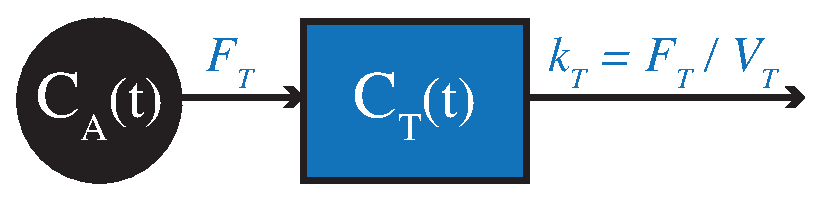
\includegraphics[width=0.5\linewidth]{OVC_diagram.eps}
    \caption{One-compartment model.}
    \label{fig:OVC_model}
    \end{figure}
    % 
    \begin{figure}[bh]\centering
    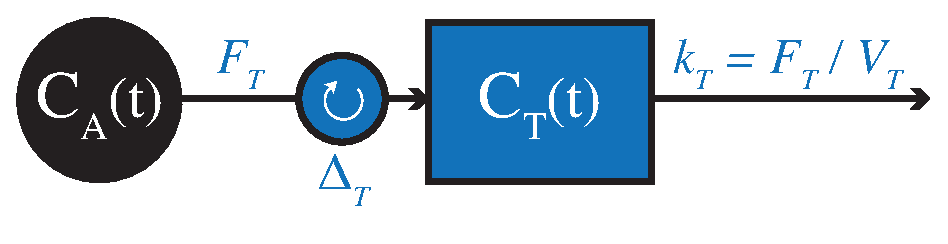
\includegraphics[width=0.5\linewidth]{OVCd_diagram.eps}
    \caption{One-compartment model with additional time-delay parameter.}
    \label{fig:OVCd_model}
    \end{figure}
    % 
    \begin{figure}[bh]\centering
    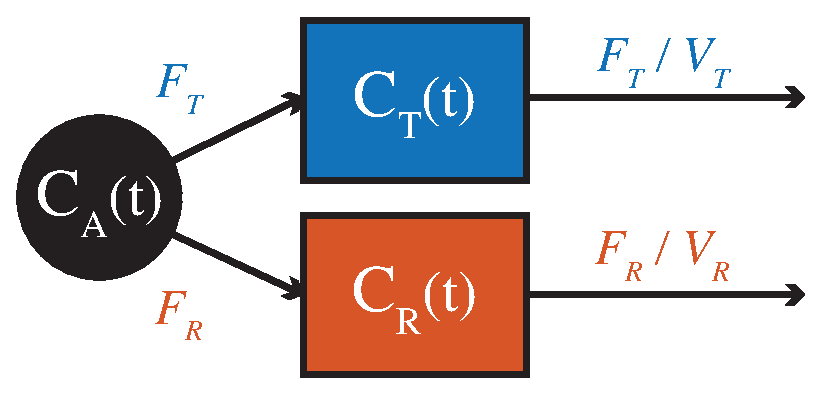
\includegraphics[width=0.5\linewidth]{rOVC_diagram.eps}
    \caption{Block diagram of the relative one-compartment model in case of a single region of interest.}
    \label{fig:rOVC_model}
    \end{figure}
    % 
    \begin{figure}[bh]\centering
    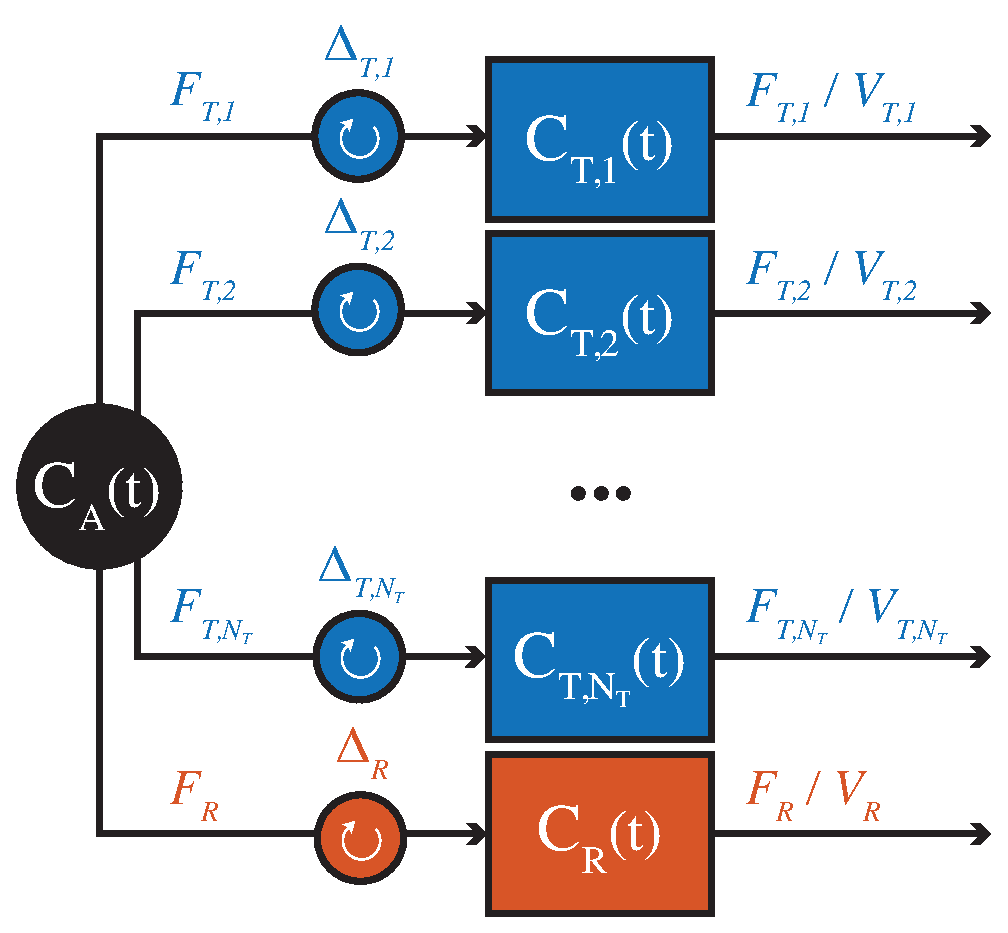
\includegraphics[width=0.5\linewidth]{rOVC_regional_diagram.eps}
    \caption{Block diagram of the relative one-compartment model for regional quantification.}
    \label{fig:rOVC_regional}
    \end{figure}
\end{subfigures}

\subsubsection{Multiplicative noise model}\label{sec:NoiseModel}
A multiplicative noise model following a gamma distribution and enforcing unit mean was used, i.e.~$\mathrm{mean}_v~p\left(v\right) = 1$, inspired by \citet{Barrois:2013gw}.
A unit mean distribution for a multiplicative noise is the equivalent of a centered distribution for additive noise.

A gamma distribution is parameterized by two parameters: the shape parameter $k$, and the scale parameter $\theta$.
Enforcing a unit mean is equivalent to set $\theta = \nicefrac{1}{k}$, the noise distribution $p\left(v\right)$ is therefore parameterized by a single shape parameter, $k$, as
\begin{equation}
p\left(v\right) = \nicefrac{1}{\Gamma\left(k\right)} ~ k^k ~ v^{k-1} ~ \mathrm e^{-vk}, \forall~v \geq 0.
\end{equation}
The shape parameter $k$ is related to the standard deviation by the relation $\sigma = \nicefrac{1}{\sqrt{k}}$, allowing modulation of the noise level in simulated TICs.
Fig.~\ref{fig:recmod} shows an example of multiplicative random noise on simulated TICs for $k = 16$, corresponding to $\sigma = 0.25$.
Unless specified differently, this value of $\sigma$ was used as the default standard deviation of the noise distribution and 150 random noise sequences were generated from this distribution.

\subsection{Quantification models}
Two different relative quantification methods, making use of a reference tissue, derived from the previously described OVC model are described. 
The following methods are intended to estimate perfusion parameters from $N_T$ tissues in a single CEUS exam.
The TIC in the i$^{th}$ tissue of interest is noted $C_T^i(t)$, where $i \in \left[\![1,N_T \right]\!]$, and the TIC in the chosen reference tissue is noted $C_R(t)$. All TICs are defined for $t \in \left[ 0, L \right]$ and count $N_S$ samples.

\subsubsection{Relative OVC model (rOVC)}
A relative OVC model can be derived from the previously presented OVC model, considering conjointly one tissue of interest with TIC $C_T^i(t)$, and one reference tissue with TIC $C_R(t)$:
\begin{equation}
\left\{
% \begin{array}{r c l}
% \frac{\mathrm dC_R \left( t - D_R \right)}{\mathrm dt} &=& F_R \frac{\mathrm dC_A \left( t \right)}{\mathrm dt} - \frac{F_R}{V_R} C_R \left( t - D_R \right), \quad \forall t \geq D_R,  \\
%  &=& 0 \textrm{ otherwise;} \\
% \frac{\mathrm dC_T \left( t - D_T \right)}{\mathrm dt} &=& F_T \frac{\mathrm dC_A \left( t \right)}{\mathrm dt} - \frac{F_T}{V_T} C_T \left( t - D_T \right), \quad \forall t \geq D_T,  \\
%  &=& 0 \textrm{ otherwise.}
% \end{array}
\begin{array}{r c l}
\dot{C_R} \left( t - D_R \right) &=& F_R \cdot C_A \left( t \right) - \frac{F_R}{V_R} \cdot C_R \left( t - D_R \right), \quad \forall t \geq D_R,  \\
 &=& 0 \textrm{ otherwise\,;} \\
\dot{C_T^i} \left( t - D_T^i \right) &=& F_T^i \cdot C_A \left( t \right) - \frac{F_T^i}{V_T^i} \cdot C_T^i \left( t - D_T^i \right), \quad \forall t \geq D_T^i,  \\
 &=& 0 \textrm{ otherwise.}
\end{array}
\right.
\label{eq:RTCM}
\end{equation}
The first equation of the system of equations (\ref{eq:RTCM}) can be rearranged as
\begin{equation}
\begin{array}{rcl}
C_A(t) &=&\frac{1}{F_{R}} \cdot \dot{C}_{R}(t - D_{R}) + \frac{1}{V_{R}} \cdot {C_{R}}(t - D_R) \quad\forall t \geq D_{R}, \\
&=& \textrm{0 otherwise.}
\end{array}
\label{eq:CACM}
\end{equation}
Figures~\ref{fig:rOVC_model} and~\ref{fig:rOVC_regional} respectively show a diagram of the \textbf{rOVC} model in case of a single tissue of interest, and in case of $N_T$ tissues of interest.

Replacing $C_A(t)$ in the second equation of system (\ref{eq:RTCM}) by its expression in equation (\ref{eq:CACM}), $\dot{C}_T^i(t)$ can be expressed as
\begin{equation}
\begin{array}{rcl}
\dot{C}_T^i \left(t - D_T^i\right) &= & \frac{F_T^i}{F_{R}} \cdot \dot{C}_{R}\left(t-D_R\right) + \frac{F_T^i}{V_R} \cdot C_{R} \left(t - D_{R}\right)  \\
& & \qquad - \frac{F_T^i}{V_T^i} \cdot C_{T^i} \left(t - D_{T^i}\right), \quad \forall t \geq D_T^i,\\
&=& \textrm{0 otherwise.}
\end{array}
\label{eq:RTDEF1}
\end{equation}

Defining the relative flow as $rF^i = \nicefrac{V_T^i}{V_R}$, the relative volume as $rV^i = \nicefrac{V_T^i}{V_R}$, and the rate constant in the i$^{th}$ tissue of interest as $k_T^i = \nicefrac{F_T^i}{V_T^i}$, the previous equation rewrites
\begin{equation}
\begin{array}{rcl}
\dot{C}_T^i \left(t - D_T^i\right) &= & rF^i \cdot \dot{C}_{R}\left(t-D_R\right) + rV^i \cdot k_T^i \cdot C_{R} \left(t - D_{R}\right) \\
& & \qquad - k_T^i \cdot C_{T}^i \left( t - D_{T}^i \right), \quad \forall t \geq D_T^i,\\
&=& \textrm{0 otherwise.}
\end{array}
\label{eq:RTDEF2}
\end{equation}

Assuming initial concentrations are equal to zero in both tissues, $\dot{C}_T^i$ in Eq.~\ref{eq:RTDEF2} integrates in exponential form~\cite{Yankeelov2005de}, yielding
\begin{equation}
\begin{array}{rcl}
C_T^i \left( t - D_T^i \right) & = & rF^i \cdot \left( k_R - k_T^i \right) \cdot \int_{0}^{t} C_{R} \left( \tau - D_R \right) \cdot e^{- k_T^i \cdot \left( t - D_R - \tau \right)} \mathrm d \tau \\
& & \qquad + rF^i \cdot C_{R} \left( t - D_R \right) \quad \forall t \geq D_T^i, \\
&=& \textrm{0 otherwise,}
\end{array}
\label{eq:RTDEF4}
\end{equation}
where $k_R = \nicefrac{F_R}{V_R}$ is the rate constant in the reference tissue.

Using such a formulation, Equation (\ref{eq:RTDEF4}) is not linearly solvable. 
A non-linear resolution method must therefore be used in order to estimate vascular parameters $rF^i$, $rV^i$, $k_T^i$, and $k_R$, in each of the $N_T$ tissues of interest, as well as the time-delay parameters $D_T^i$, and $D_R$.
This approach has been investigated in Chapters~\ref{chapter:PMB} and~\ref{chapter:PMB2}, and was therefore not included in the study. 
Instead we used the linear formulation presented in the following Section.
\FloatBarrier

\subsubsection{Linear resolution of the rOVC model (rLin)}\label{sec:rLin}
Alternatively, under similar assumptions, $\dot{C}_T^i$ in Eq.~\ref{eq:RTDEF2} can be integrated over time, yielding the following expression of $C_T^i$~\cite{CardenasRodriguez:2013em}
\begin{equation}
\begin{array}{rcl}
C_T^i \left(t - D_T^i\right) &=& rF^i \cdot C_{R}\left(t-D_R\right) + rV^i \cdot k_T^i \cdot \int_0^t C_{R} \left(\tau - D_{R}\right) \mathrm d\tau \\
& & \qquad - k_T^i \cdot \int_0^t C_{T}^i \left( \tau - D_{T}^i \right) \mathrm d\tau, \quad \forall t \geq D_T^i,\\
&=& \textrm{0 otherwise.}
\end{array}
\label{eq:RTDEF3}
\end{equation}

Assuming time delay parameters $D_T^i$ and $D_R$ are estimated beforehand using the method presented in Section~\ref{sec:estimationDelay}, TICs can be time-shifted, mimicking an ideal case with no delay in bolus arrival.
Variables $x^i\left(t\right)$, $y^i\left(t\right)$ are time-shifted versions of the TIC in the i$^{th}$ tissue of interest and its integral.
They are defined $\forall t \in \left[ 0,\,L-D_T^i\right]$, as
\begin{equation}
\begin{array}{rcl}
x^i\left(t\right) &=& C_{T}^i\left(t + D_T^i\right), \\
y^i\left(t\right) &=& -\int_0^{t} C_{T}^i \left( \tau + D_T^i \right) \mathrm d\tau.
\end{array}
\label{eq:RTLINV1}
\end{equation}
Similarly, variables $u\left(t\right)$, $v\left(t\right)$ are time-shifted versions of the reference TIC and its integral.
They are defined $\forall t \in \left[ 0,\,L-D_R\right]$, as
\begin{equation}
\begin{array}{rcl}
u\left(t\right) &=& C_{R}\left(t + D_R\right), \\
v\left(t\right) &=& \int_0^t C_{R} \left(\tau + D_R \right) \mathrm d\tau.
\end{array}
\label{eq:RTLINV2}
\end{equation}

Eq.~\ref{eq:RTDEF3} can be interpreted as an overdetermined system of $N_S$ linear equations~\cite{Bjorck:1996uz}, i.e.~one equation for each time sample $t$.
It can therefore be written
\begin{equation}
x^i\left(t\right) = a^i \cdot u\left(t\right) + b^i \cdot v\left(t\right) + c^i \cdot y^i\left(t\right) \qquad \forall t \geq D_T^i,
\label{eq:RTLINF}
\end{equation}
where coefficients $a^i$, $b^i$, and $c^i$ are defined as
\begin{equation}
a^i = rF^i, \quad b^i = rV^i \cdot k_T^i, \quad c^i = k_T^i.
\label{eq:RTLINC}
\end{equation}

The system can be solved using a linear least-squares resolution method, yielding estimates of parameters $a^i$, $b^i$, and $c^i$ by minimization of the squared fit error $\varepsilon^i$
\begin{equation}
\argmin_{\left\lbrace a^i, b^i, c^i\right\rbrace} \varepsilon^i, \textrm{ where } \varepsilon^i = \sum_t \Big( x^i\left(t\right) - a^i\cdot u\left(t\right) - b^i\cdot v\left(t\right) - c^i\cdot y^i\left(t\right) \Big)^2.
\end{equation}
Vascular parameters of the \textbf{rLin} model can then be derived easily using
\begin{equation}
rF^i = a^i,~rV^i = \nicefrac{b^i}{c^i}, \textrm{ and } k_T^i = c^i.
\end{equation}

The linear resolution of the \textbf{rOVC} model will be referred to as \textbf{rLin} in the following.
For the case of a single region, $N_T = 1$, the \textbf{rLin} model is equivalent to the method proposed by \citet{CardenasRodriguez:2013em}.

\subsubsection{Regularized linear resolution of the rOVC model (rReg)}
Estimating $rF^i$, $rV^i$, and $k_T^i$ in $N_T$ tissues using the \textbf{rLin} model, $N_T$ values of parameter $k_R$ can be derived as a linear combination of the \textbf{rLin} model parameters:
\begin{equation}
k_R = \frac{F_R}{F_T^i}\frac{F_T^i}{V_T^i}\frac{V_T^i}{V_R} = \frac{rV^i \cdot k_T^i}{rF^i} = \frac{b^i}{a^i}
\label{eq:KR}
\end{equation}

When there are more than one tissue of interest ($N_T > 1$), $N_T$ values of parameter $k_R$ can be derived from the parameters of the \textbf{rLin} model. 
However, these $N_T$ values of $k_R$ characterize the same reference tissue, associated to a single reference TIC $C_R\left(t\right)$. 
A unique value of $k_R$ should therefore be estimated per exams in order to avoir discrepancies between the $N_T$ tissues of interest.

The linear relation between parameters of the \textbf{rLin} model provided by Eq.~\ref{eq:KR} can be used as a constraint to ensure the $N_T$ derived values of $k_R$ are consistent across tissues.
Substituting in Eq.~\ref{eq:RTLINF} yields 
\begin{equation}
\begin{array}{rcl}
x^i\left(t\right) &=& a^i\cdot\left( u\left(t\right) + k_R\cdot v\left(t\right)\right) + c^i\cdot y^i\left(t\right),
\end{array}
\label{eq:RTREG}
\end{equation}
which rewrites 
\begin{equation}
\begin{array}{rcl}
x^i\left(t\right) &=& a^i\cdot w\left(t\right) + c^i\cdot y^i\left(t\right)
\end{array}
\label{eq:RTREG2}
\end{equation}
where $w\left(t\right)$ is defined by
\begin{equation}
\begin{array}{rcl}
w\left(t\right) &=& u\left(t\right) + k_R \cdot v\left(t\right),\\
&=& C_{R}\left(t-D_R\right) + k_R \cdot \int_0^t C_{R} \left(\tau - D_{R}\right) \mathrm d\tau.
\end{array}
\label{eq:RTREG3}
\end{equation}

When a value of parameter $k_R$ is provided, the $N_T$ linear system equations defined in Eq.~\ref{eq:RTREG} are independently solvable using a linear least-squares resolution method, minimizing the squared error, $e^i$:
\begin{equation}
\argmin_{\left\lbrace a^i, c^i \right\rbrace} e^i, \textrm{ where } e^i = \sum_{t} \Big( x^i\left(t\right) - \left[a^i\cdot w\left(t\right) + c^i\cdot y^i\left(t\right) \right] \Big)^2.
\end{equation}

Since the value of $k_R$ is necessary to define $w\left(t\right)$, its value must be determined.
We proposed a non-linear iterative optimization scheme that estimates the value of $k_R$ by iteratively minimizing the normalized mean squared error, $E$:
\begin{equation}
\argmin_{k_R} E, \textrm{ where } E = \sum_i\frac{\sqrt{\nicefrac{e^i}{N_S^i} }}{\lvert x^i\left(t\right) \rvert_{\infty}},
\end{equation}
$N_S^i$ being the number of samples in $x^i(t)$, i.e.~the number of time samples verifying $t \in \left[0,\,L-D_T^i\right]$, and $\lvert x^i\left(t\right) \rvert_{\infty}$ is the uniform norm of $x^i\left(t\right)$ defined as the maximum absolute value in the regional time-shifted curve.
Vascular parameters were then derived from the model estimates as 
\begin{equation}
rF^i = a^i,~rV^i = \frac{k_R \cdot a^i}{c^i}, \textrm{ and } k_T^i = c^i.
\end{equation}

\subsubsection{Estimation of time-delay parameters}\label{sec:estimationDelay}
As stated in the presentation of the \textbf{rLin} and \textbf{rReg} models, time-delay parameters are known beforehand, and TICs shifted in time in order to correct for time-delays prior to solving the linear system of equations.
The determination method of the time-delay parameter, noted $D$, of a generic TIC, noted $C\left(t\right)$, was defined in order to determine the time of arrival of the first microbubbles in the tissue of interest.
This is a difficult task because of the noise present in data. 
We propose here an empirical estimation method adapted to contrast-enhanced ultrasound data.

$C\left(t\right)$ was noise-filtered twice by a moving-average filter of width 2 seconds, yielding $C_f\left(t\right)$.
The time $t_{20\%}$ at which $C_f\left(t\right)$ reaches 20\% of its maximum value sets an upper bound of $D$.
$C_f\left(t\right)$ was then truncated, keeping only the part where $t \leq t_{20\%}$.
The derivative of $C_{f}\left(t\right)$, noted $\dot{C}_{f}\left(t\right)$, was approximated by convolution of the TIC with the central difference operator~\cite{Whittaker:2008wv}. % Whittaker, E. T. and Robinson, G. "Central-Difference Formulae." Ch. 3 in The Calculus of Observations: A Treatise on Numerical Mathematics, 4th ed. New York: Dover, pp. 35-52, 1967.
Finally, assuming no oscillation occurred in the TIC prior to bolus arrival, $D$ was defined as the time at which the derivative $\dot{C}_{f}\left(t\right)$ reaches 20\% of its value at $t = t_{20\%}$:
\begin{equation}
D \leq t_{20\%}\,\wedge\,\dot{C}_{f}\left(D\right) = 0.2 \times \dot{C}_{f}\left(t_{20\%}\right).
\end{equation}

\section{Materials and Methods}
\subsection{Simulations of CEUS data}
\subsubsection{Simulation process}
Regional perfusion parameters were derived from experimental data fitted with the \textbf{OVC} model presented in Section~\ref{sec:OVCModel}.
The arterial input function was derived from a preclinical study using the segmentation method presented in Chapter~\ref{chapter:PMB}.
A log-normal model was fitted to the resulting arterial curve for noise-filtering purposes. 
Regional enhancement curves corresponding to different tissues of interest were simulated using the \textbf{OVC} model, along with the model parameters estimated in different regions of the tumor, and the arterial input function.
A reference tissue region was similarly simulated.
The perfusion parameters of the \textbf{OVC} model used for simulation are presented in Figure~\ref{fig:simRef}.
The associated time-intensity curves simulated for each tumor region, as well as for the reference tissue are displayed in Figure~\ref{fig:simCtCr}.

\begin{figure}[bh]
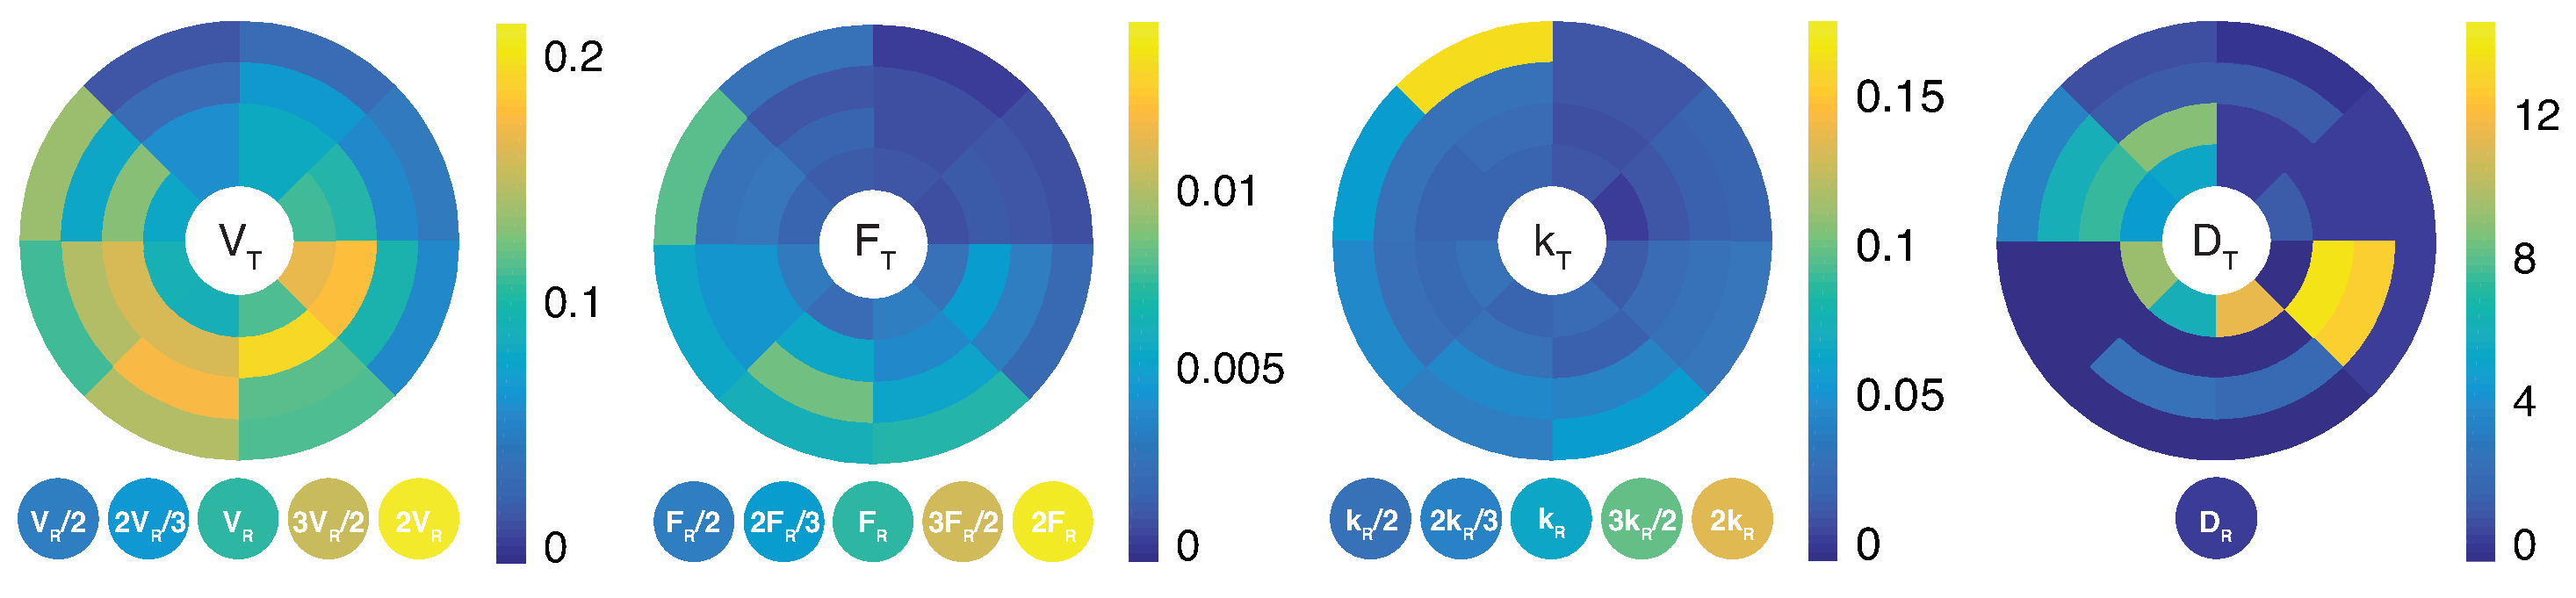
\includegraphics[width=\linewidth]{simRef.eps}
\caption{Absolute perfusion parameters used for simulation with the OVC model, i.e.~tissue blood volume, $V_T$ and $V_R$ (dimensionless), tissue blood flow, $F_T$ and $F_R$ (in $s^{-1}$), tissue rate constant, $k_T$ and $k_R$ (expressed in $s^{-1}$), and time delay, $D_T$ and $D_R$ (in $s$). Bullseye view of the parameters in the 32 tumor regions. The bottom disks represent the parameters used to simulated the reference tissue region, the middle disk being the original value used for all experiments. The other disks are, from left to right, the half, two thirds, three halves, and double of the original value, used to study the influence of the reference tissue.}
\label{fig:simRef}
\end{figure}

\begin{figure}
\includegraphics[width=\linewidth]{simCtCr.eps}
\caption{Time-intensity curves inside of each of the 32 tumor regions (top grid), and in the reference tissue (bottom), simulated using the \textbf{OVC}. Each plot shows the simulated noiseless curve (orange line) in the region, i.e.~$\sigma = 0$, as well as the curve with simulated multiplicative noise (blue dots), i.e.~$\sigma = 0.25$.}
\label{fig:simCtCr}
\end{figure}
\FloatBarrier

\subsubsection{Varying factors}
\paragraph{Noise level}
The influence of noise was investigated by varying parameter $\sigma$, i.e.~the standard deviation of the multiplicative noise model.
$\sigma$ was varied linearly with increments of 0.05 from 0, corresponding to a noiseless conditions, to 0.5, corresponding to high noise conditions.
For each noise level, 150 random noise sets following the multiplicative gamma noise model were generated.

\paragraph{Exam duration}
Various exam durations were investigateds by varying the number of samples in the simulated data.
The exam duration was varied from 50 seconds to 165 seconds with 5 seconds increments.

\paragraph{Sampling period}
Simulated noiseless enhancement curves were resampled using varying sampling periods to study the impact of this parameter on the accuracy and precision of the estimation.
The sampling period was varied from 0.1 to 1.0 second with 0.1 increments, this range being representative of the acquisition settings that can be found in contrast-enhanced ultrasound studies.

\paragraph{Reference tissue}
The reference tissue is characterized by the parameters of the OVC model, i.e.~$V_R$, $F_R$ (and thus $k_R = \dfrac{F_R}{V_R}$).
The impact of these parameters on the accuracy and the precision of the quantification process using the \textbf{rLin} and the \textbf{rReg} models was investigated.
In particular, the tissue blood volume, the tissue blood flow of the reference tissue were varied by scaling either or both of them by $\dfrac{1}{2}$, $\dfrac{2}{3}$, $1$, $\dfrac{3}{2}$, and $2$.
Because of the relation between the three parameters, they cannot be varied individually.
It is however possible to fix one of the parameters while varying the two others.
The disks at the bottom Figure~\ref{fig:simRef} shows the various values of the perfusion parameters used to simulate the reference tissue enhancement curve, the middle disk being the value obtained from experimental data, i.e.~the values which were used for the other simulations.

\paragraph{Number of regions}
Various regional segmentation were performed varying the number of tumor regions as powers of two, ranging from 1 to 32.
For each segmentation, the parameters of the OVC model were estimated using the mean enhancement curve in each corresponding tumor region.
Figure~\ref{fig:simReg} shows the simulated values of the perfusion parameters for the various segmentations with a varying number of regions. 
The absolute perfusion parameters of the OVC model were used to derive the parameters of the rOVC model using the definitions of Eq.~\ref{eq:RTDEF2}.
The derived parameters were then used as ground truth to evaluate the accuracy of the perfusion parameters estimated using the \textbf{rLin} and the \textbf{rReg} models.

\begin{figure}
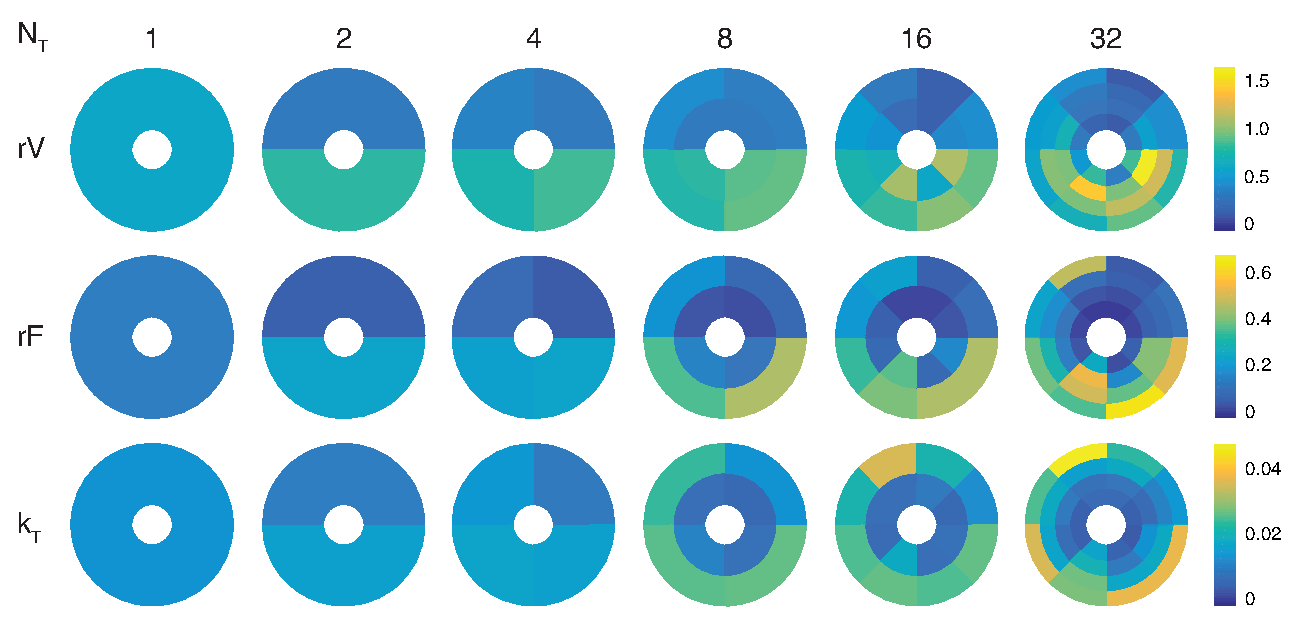
\includegraphics[width=\linewidth]{simReg_sim.eps}
\caption{Relative perfusion parameters used for simulation varying the number of tumor regions $N_T$ from 1 (left) to 32 (right), i.e.~relative tissue blood volume, $rV$, relative tissue blood flow, $rF$, tissue rate constant, $k_T$.}
\label{fig:simReg}
\end{figure}

\subsection{Data analysis}\label{sec:dataAnalysis}
The accuracy and the precision of the parameters estimated using the \textbf{rLin} and the \textbf{rReg} models were respectively investigated through the median value, and either the standard deviation or the interquartile range, of the relative estimation error over 150 random noise samples.
The relative estimation error of parameter $\theta$, noted $rE_{\theta}$, is expressed in percent and defined as
\begin{equation}
rE_{\theta} = 100 \times \frac{\theta_{est}-\theta_{sim}}{\theta_{sim}}
\end{equation}
i.e.~the difference between the estimated parameter $\theta_{est}$ and the simulated parameter $\theta_{sim}$, normalized by the simulated value.
\FloatBarrier

\section{Results}
In this section we present the results of our simulation experiments.
Figure~\ref{fig:gridIndices} provides the correspondance between regions, depending on the type of data to be presented.
Indeed, color-coded bullseyes were used when a single value had to be represented per region, but grids of plots were used to show the regional results as a function of a simulation parameter, i.e.~noise level, exam duration, and sampling period.

In Figures~\ref{fig:noise_rV} to \ref{fig:sampling_kR}, each plot represents a tumor region, i.e.~the top row corresponds to the outer rim and the bottom row to the inner rim, the columns correspond to the clockwise ordering of the regions on a rim starting with the left region above the horizontal line.

\begin{figure}
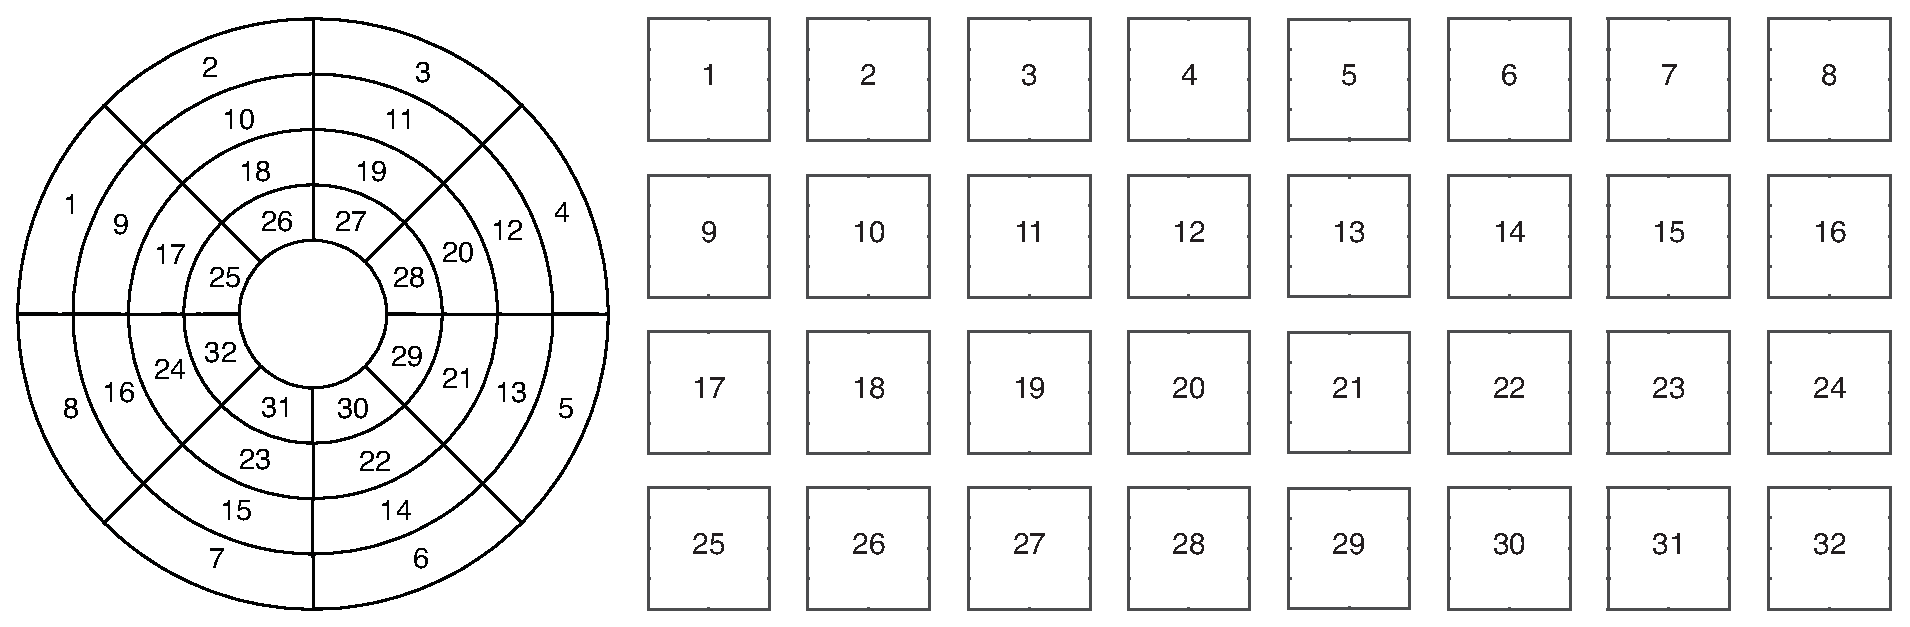
\includegraphics[width=\linewidth]{gridIndices.eps}
\caption{Correspondance of the regions between bullseye (left) and grid (right) representation.}
\label{fig:gridIndices}
\end{figure}
\FloatBarrier

\subsection{Noise level}
Figures~\ref{fig:noise_rV} to \ref{fig:noise_kR} show the relative estimation error of the relative tissue blood volume (Figure~\ref{fig:noise_rV}), relative tissue blood flow (Figure~\ref{fig:noise_rF}), and rate constants in the tumor (Figure~\ref{fig:noise_kT}) and reference  (Figure~\ref{fig:noise_kR}) tissues obtained using the \textbf{rLin} and \textbf{rReg} models, as a function of the noise level simulated in the data, i.e.~the standard deviation of the multiplicative noise model.

Expectedly, for the four parameters of both models, the interquartile range of the relative estimation bias increased with the noise level, and no relation was found between the noise level and the median value of the relative estimation error.
In terms of relative tissue blood volume (see Figure~\ref{fig:noise_rV}), the two models were hardly differenciable.
Inside a given region, the median relative estimation error value can be different with a slight advantage for the \textbf{rLin} model, but the precision of the estimation is however generally comparable.
Additionally, the \textbf{rReg} model makes the estimation bias of $rV$ more consistent across regions.
Regarding relative blood flow (see Figure~\ref{fig:noise_rF}), the \textbf{rLin} model was generally more accurate than the \textbf{rReg} model. 
However the estimation of $rF$ was less precise and more sensitive to noise using the \textbf{rLin} model.
In terms of the rate constant in tumor tissues (see Figure~\ref{fig:noise_kT}), the \textbf{rReg} model proved both more accurate and more precise than the \textbf{rLin} model.
Indeed, the \textbf{rReg} model exhibited an extremely consistent estimation bias across regions, with an average of -3\%, and a lower sensitivity to noise.
The \textbf{rLin} model on the other hand, yielded estimates of $k_T$ with highly variable biases, i.e.~the median bias reaching 40\% in one of the regions, and overestimating the parameter in some regions while underestimating it in others.
A common value of the rate constant in the reference tissue (see Figure~\ref{fig:noise_kR}), $k_R$, was estimated for all tumor regions using the \textbf{rReg} model.
The regularized model underestimated $k_R$ by 5\% in average in our experiments and exhibited a rather low sensitivity to noise. 
Oppositely, the estimates of the \textbf{rLin} model were extremely inconsistent across regions, and were more sensitive to noise in most regions.

\begin{subfigures}
    \begin{figure}\centering
        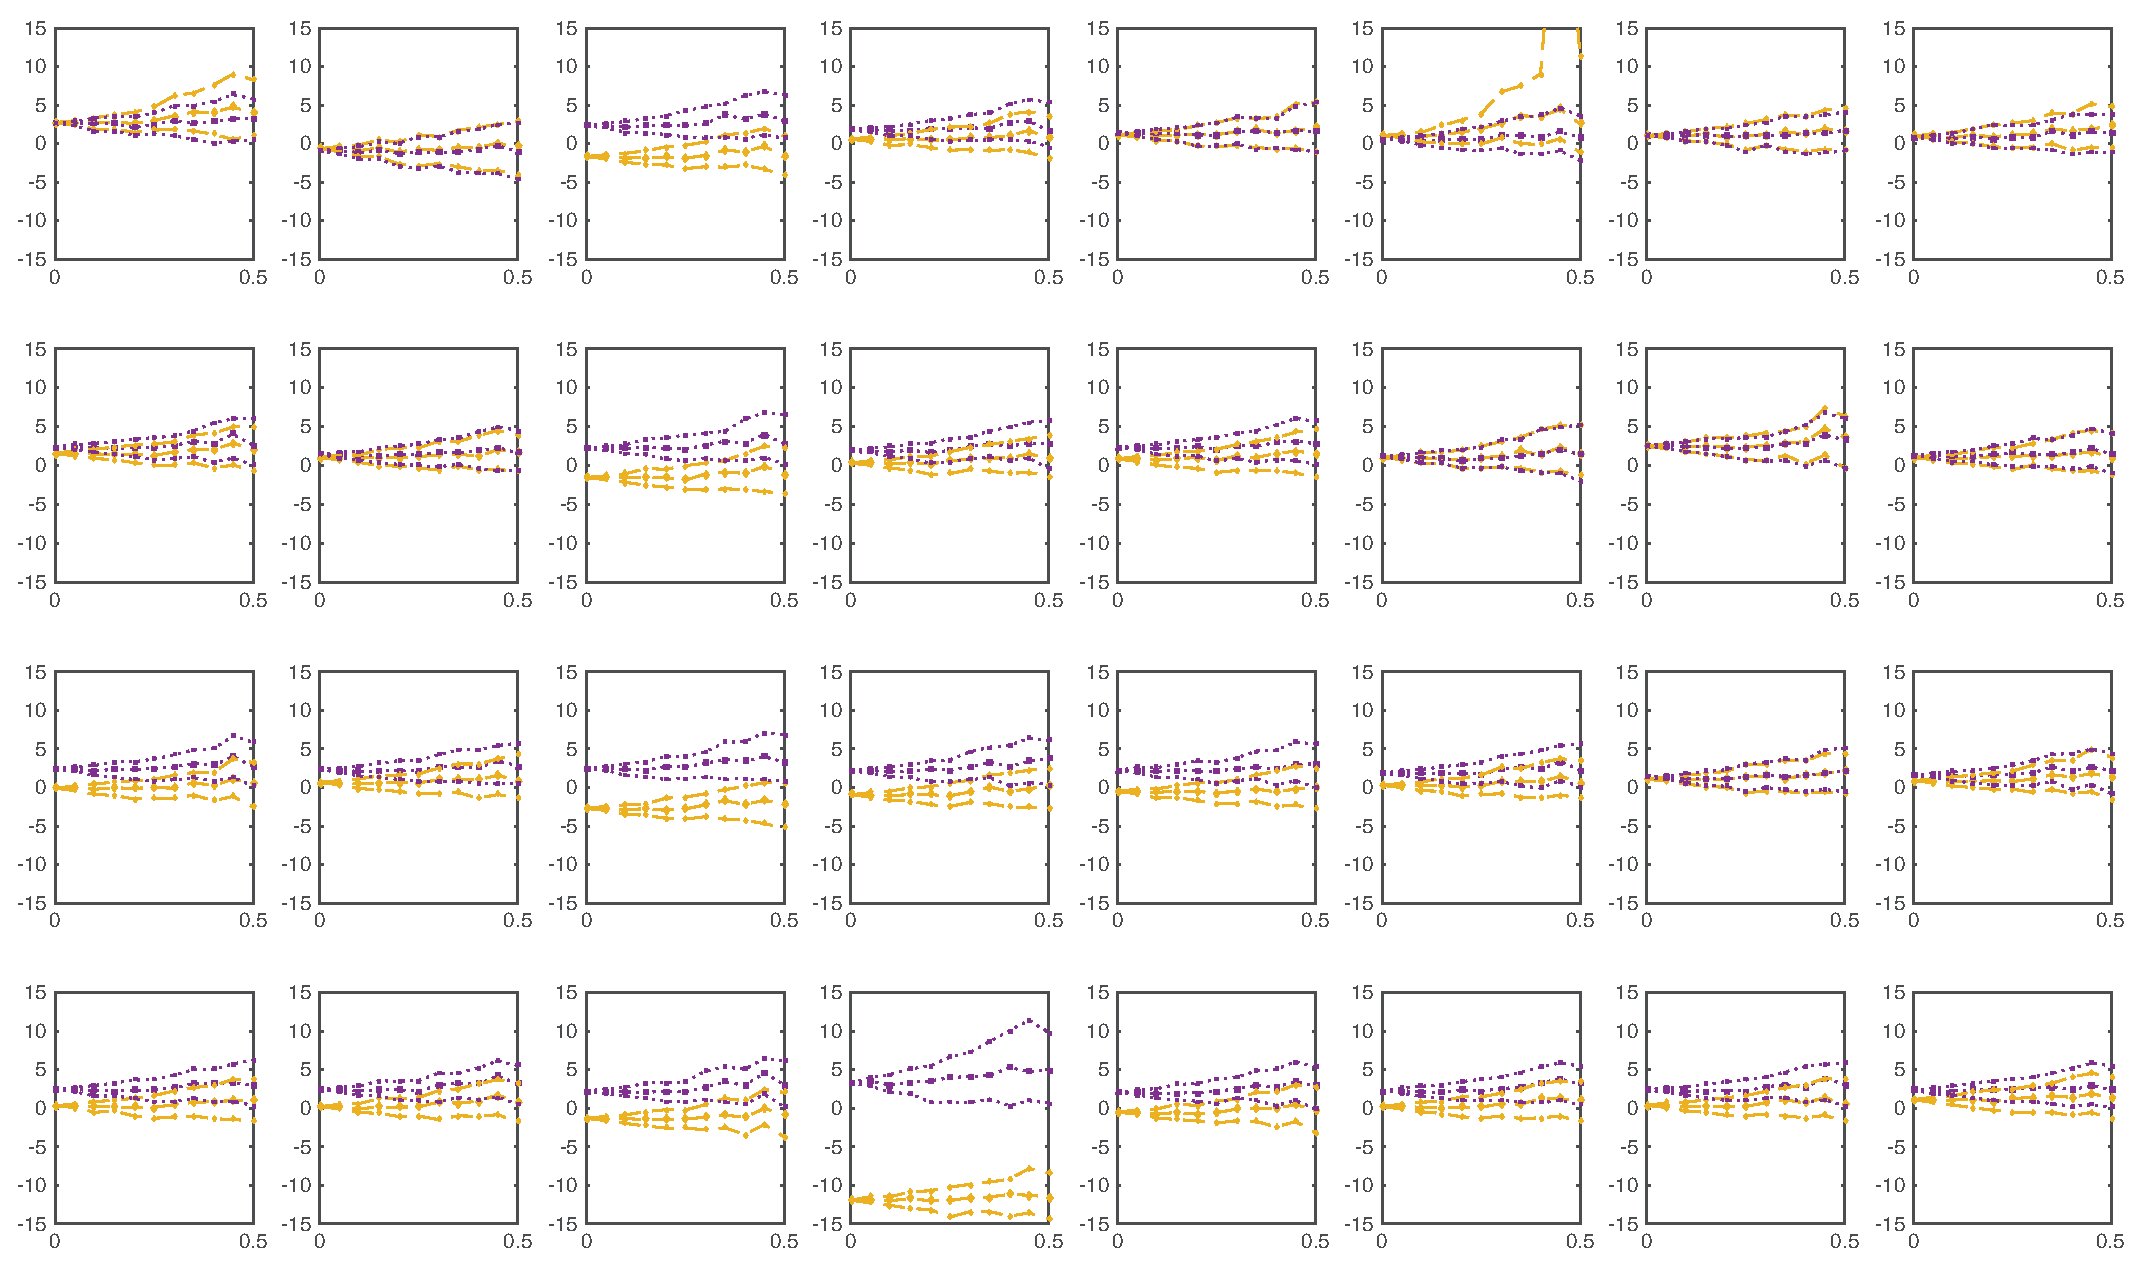
\includegraphics[width=0.95\linewidth]{simNoise_rV.eps}
        \caption{Median (large symbols) and first and third quartiles (small symbols) of the relative estimation error for the relative blood volume ($rV$) estimated in the 32 tumor regions using the \textbf{rLin} (yellow diamonds) and \textbf{rReg} (purple squares) models, as a function of the noise level.}
        \label{fig:noise_rV}
    \end{figure}
    \begin{figure}\centering
        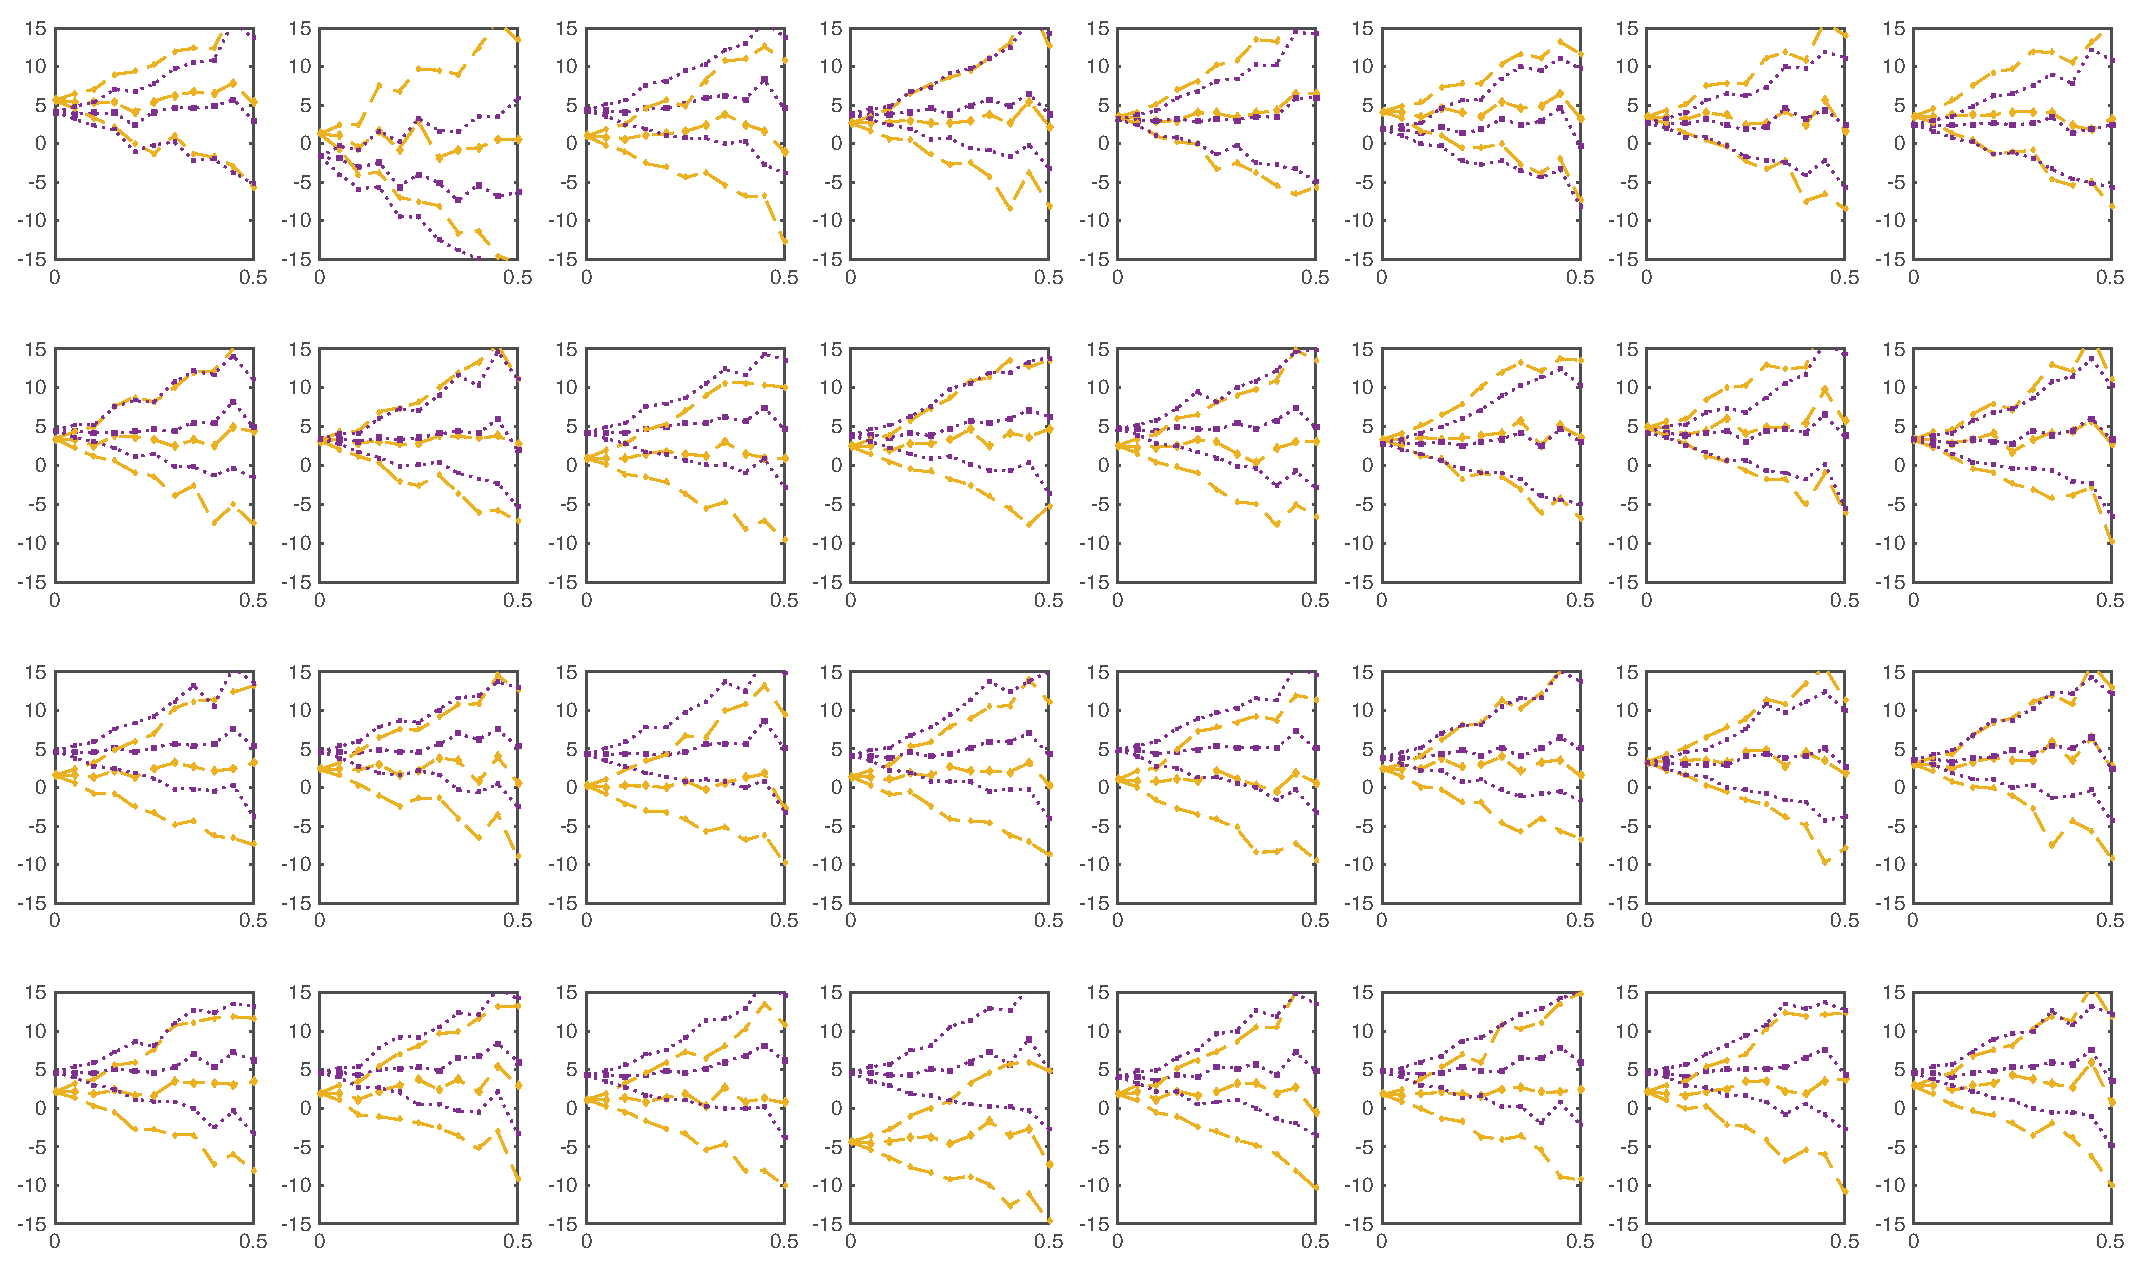
\includegraphics[width=0.95\linewidth]{simNoise_rF.eps}
        \caption{Median (large symbols) and first and third quartiles (small symbols) of the relative estimation error for the relative blood flow ($rF$) estimated in the 32 tumor regions using the \textbf{rLin} (yellow diamonds) and \textbf{rReg} (purple squares) models, as a function of the noise level.}
        \label{fig:noise_rF}
    \end{figure}
    \begin{figure}\centering
        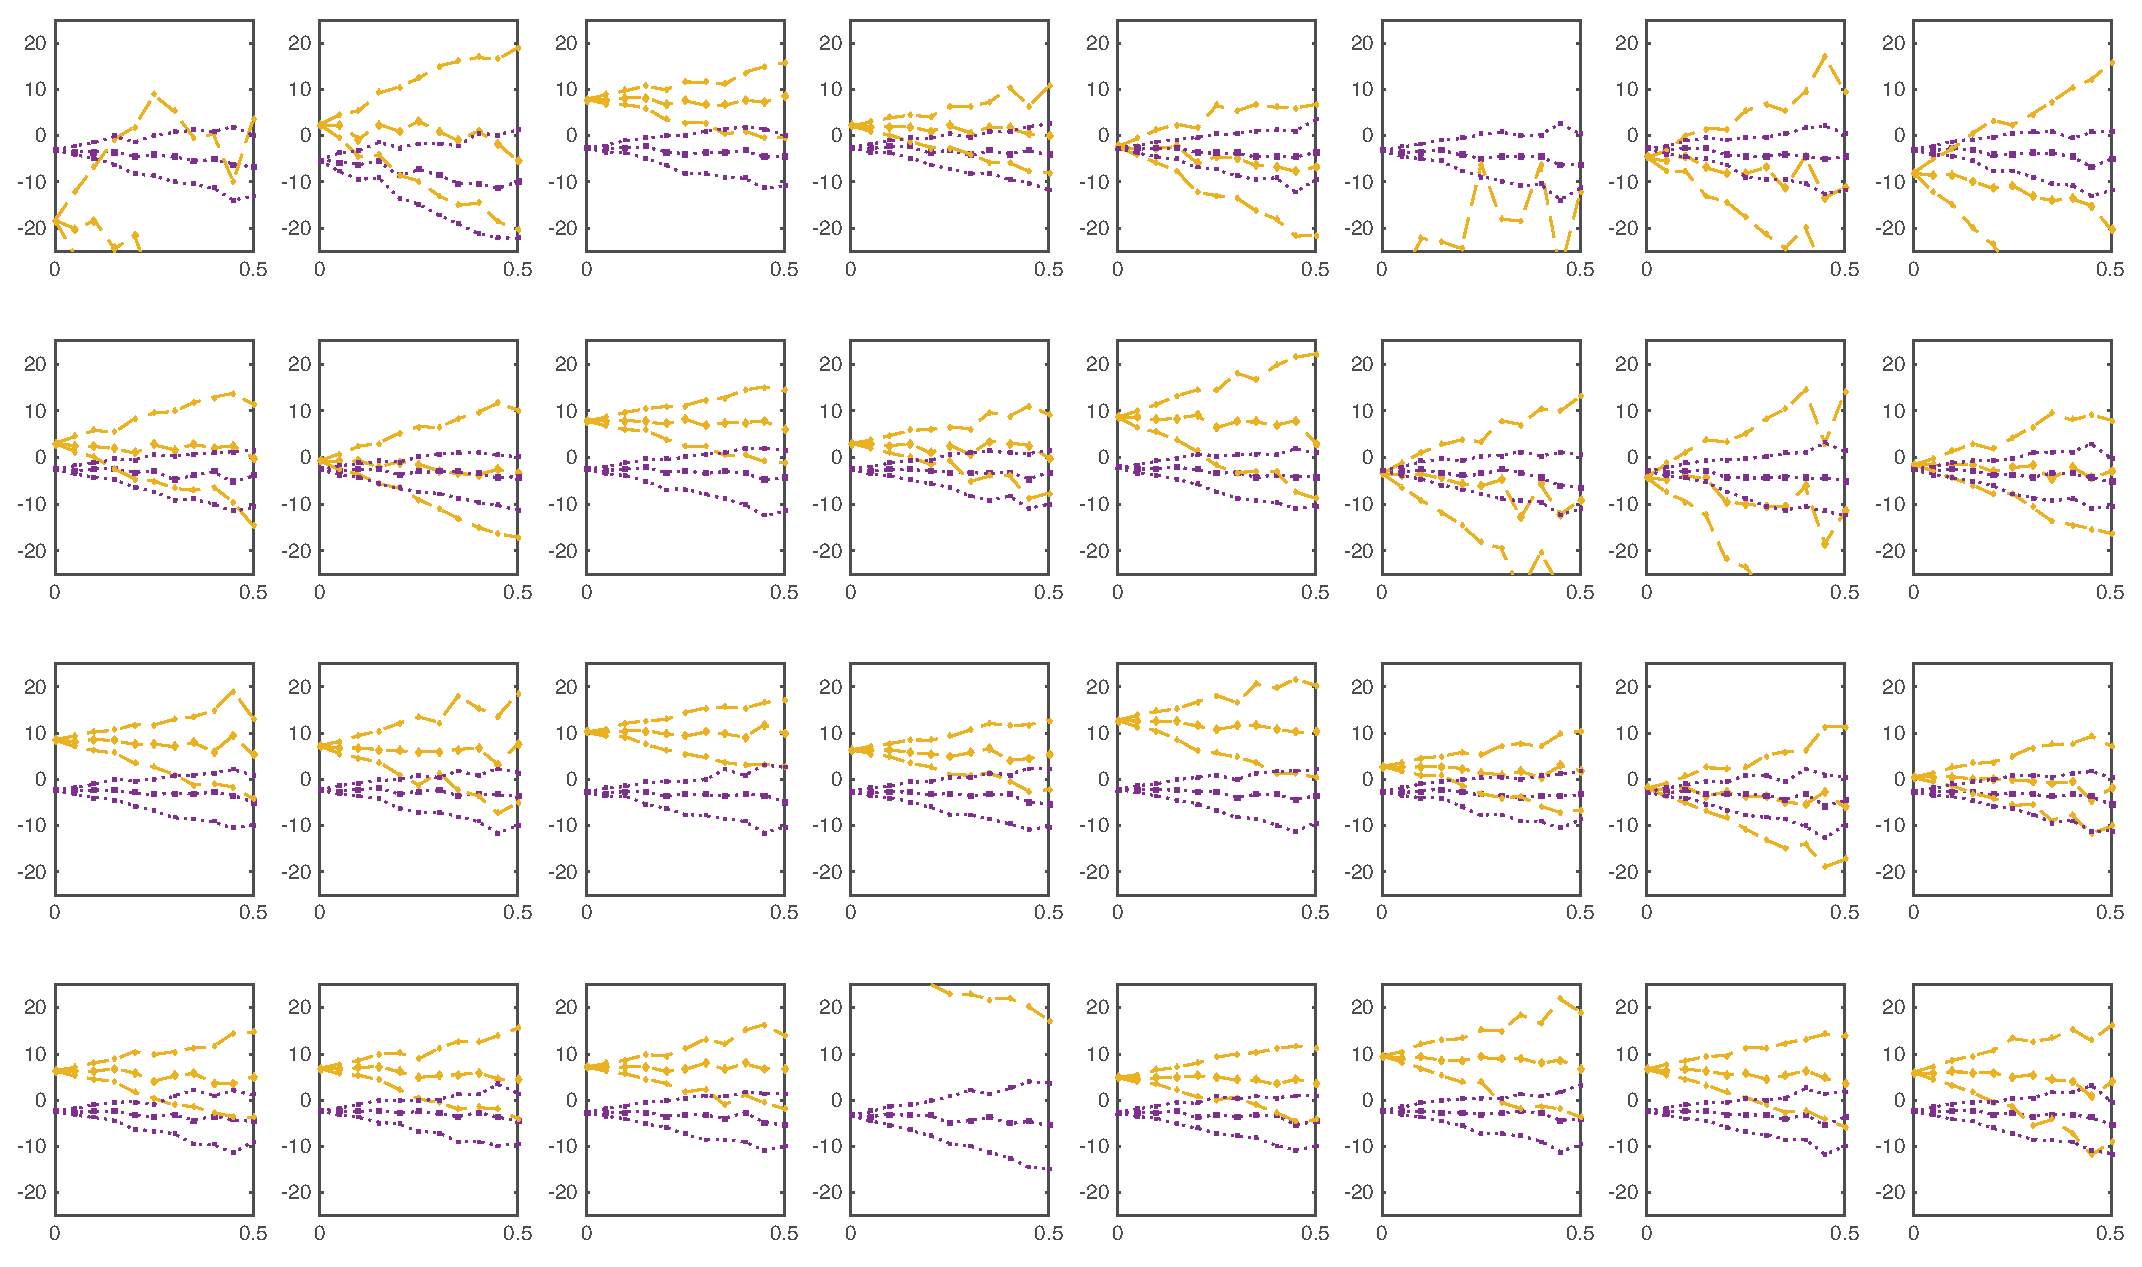
\includegraphics[width=0.95\linewidth]{simNoise_kT.eps}
        \caption{Median (large symbols) and first and third quartiles (small symbols) of the relative estimation error for the rate constant in the tumor ($k_T$) estimated in the 32 tumor regions using the \textbf{rLin} (yellow diamonds) and \textbf{rReg} (purple squares) models, as a function of the noise level.}
        \label{fig:noise_kT}
    \end{figure}
    \begin{figure}\centering
        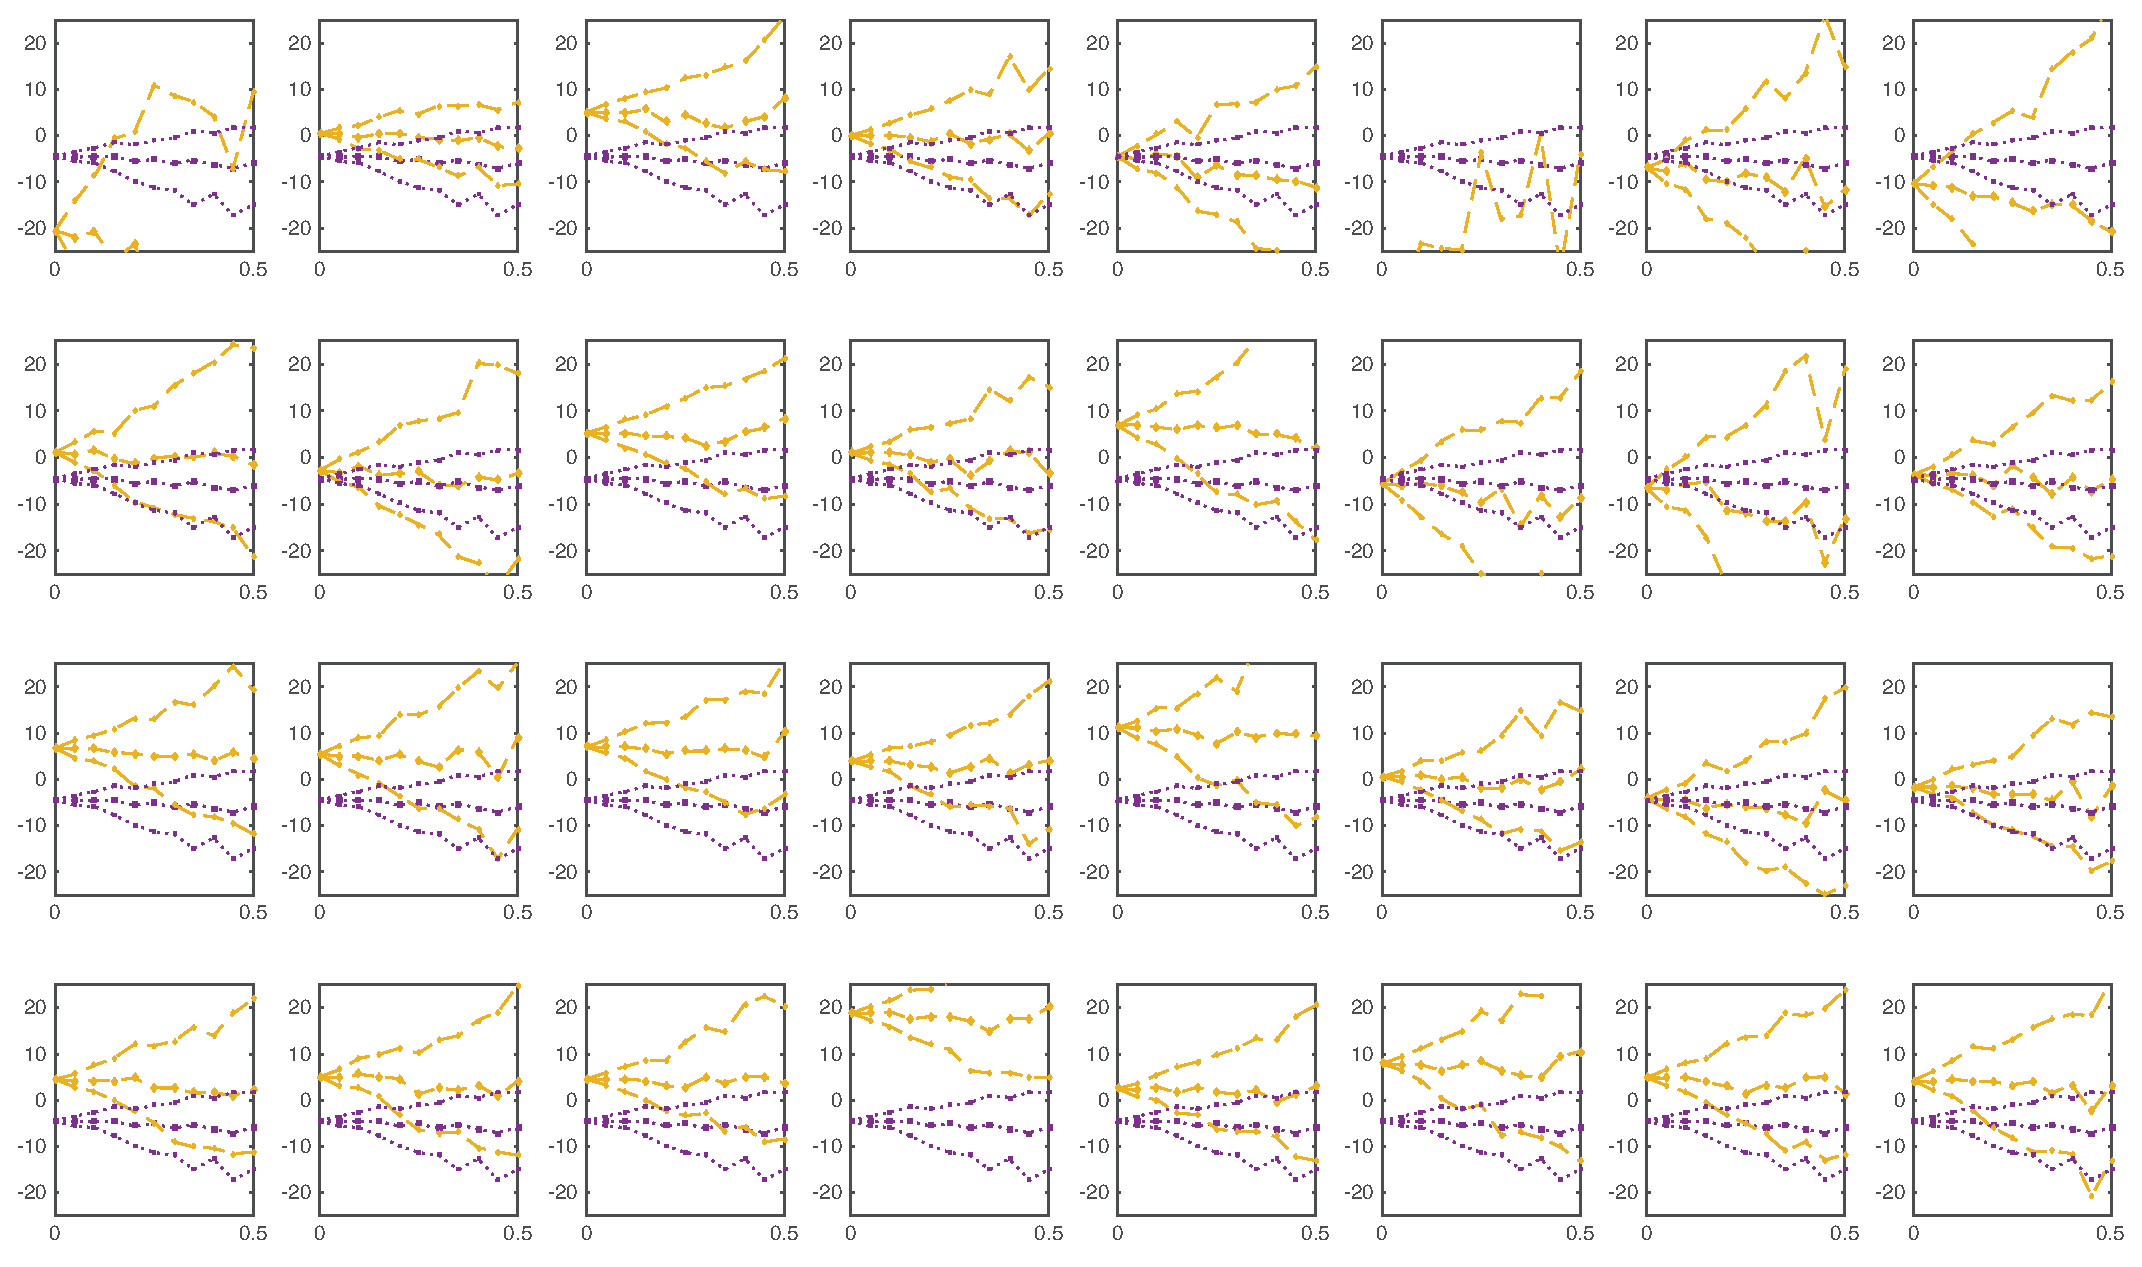
\includegraphics[width=0.95\linewidth]{simNoise_kR.eps}
        \caption{Median (large symbols) and first and third quartiles (small symbols) of the relative estimation error for the rate constant in the reference tissue ($k_R$) estimated in the 32 tumor regions using the \textbf{rLin} (yellow diamonds) and \textbf{rReg} (purple squares) models, as a function of the noise level.}
        \label{fig:noise_kR}
    \end{figure}
\end{subfigures}
\FloatBarrier

\subsection{Exam duration}
Figures~\ref{fig:examDuration_rV} to \ref{fig:examDuration_kR} show the impact of the exam duration on the relative estimation error of the perfusion parameters of the \textbf{rLin} and \textbf{rReg} models, i.e.~relative tissue blood volume (Figure~\ref{fig:examDuration_rV}), relative tissue blood flow (Figure~\ref{fig:examDuration_rF}), and rate constants in the tumor (Figure~\ref{fig:examDuration_kT}) and in the reference tissue (Figure~\ref{fig:examDuration_kR}).

Regarding relative blood volume (see Figure~\ref{fig:examDuration_rV}), the \textbf{rReg} model was able to estimate the parameter accurately, and to reach a steady state with exams as short as 80 seconds for the simulated noise level, i.e.~$\sigma = 0.25$.
Oppositely, the \textbf{rLin} model only yielded accurate estimates using the whole exam duration, i.e.~165 seconds, and at the exception of one region it overall underestimated $rV$.
Comparably, the relative blood flow (see Figure~\ref{fig:examDuration_rF}) was steadily estimated using the \textbf{rReg} model with exams as short as 50 seconds, despite an average overestimation of less than 4\%.
The estimates of $rF$ given by the \textbf{rLin} were found more sensitive to the duration of the exam, and generally overestimated $rF$ for very short exams, the estimates first decreasing and then increasing linearly with the exam duration.
Regarding the rate constant in the tumor (see Figure~\ref{fig:examDuration_kT}), the \textbf{rLin} model was unable to accurately estimate the parameter for incomplete exams, and exhibited strong biases in short exams, again varying from one exam to another. 
The \textbf{rReg} model was able to steadily and uniformely estimate parameter $k_T$, despite the tendency of the median relative estimation error to slightly decrease with the exam duration for exams lasting more than 100 seconds.
Moreover, the estimation of $k_T$ was more precise using the \textbf{rReg} model.
For both models, the bias in the estimation of $k_R$, the rate constant in the reference tissue (see Figure~\ref{fig:examDuration_kR}), was strongly correlated to the bias in the estimation of $k_T$.

\begin{subfigures}
    \begin{figure}\centering
        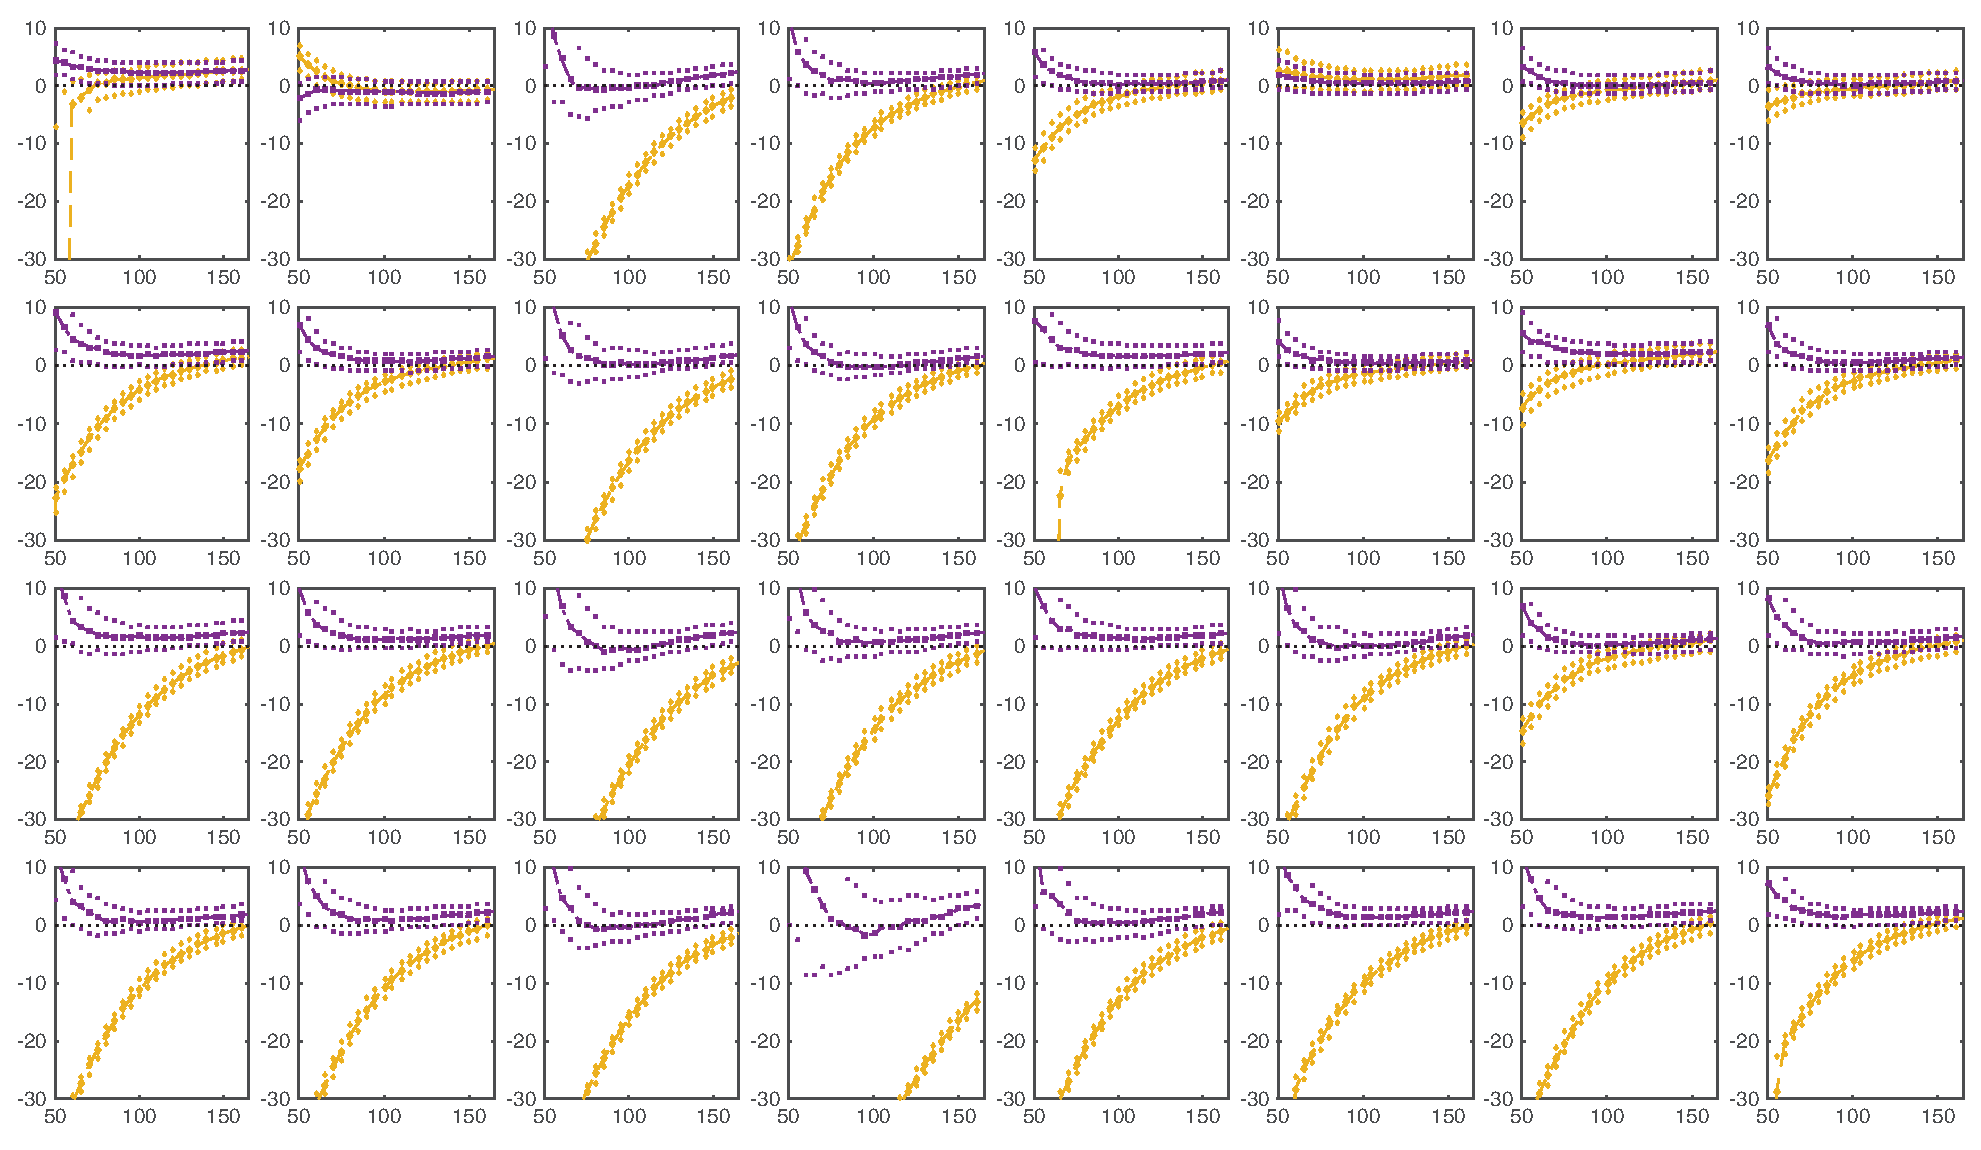
\includegraphics[width=0.95\linewidth]{simSamples_rV.eps}
        \caption{Median (large symbols) and first and third quartiles (small symbols) of the relative estimation error for the relative blood volume ($rV$) estimated using the \textbf{rLin} (yellow diamonds) and \textbf{rReg} (purple squares) models, as a function of the exam duration.}
        \label{fig:examDuration_rV}
    \end{figure}
    \begin{figure}\centering
        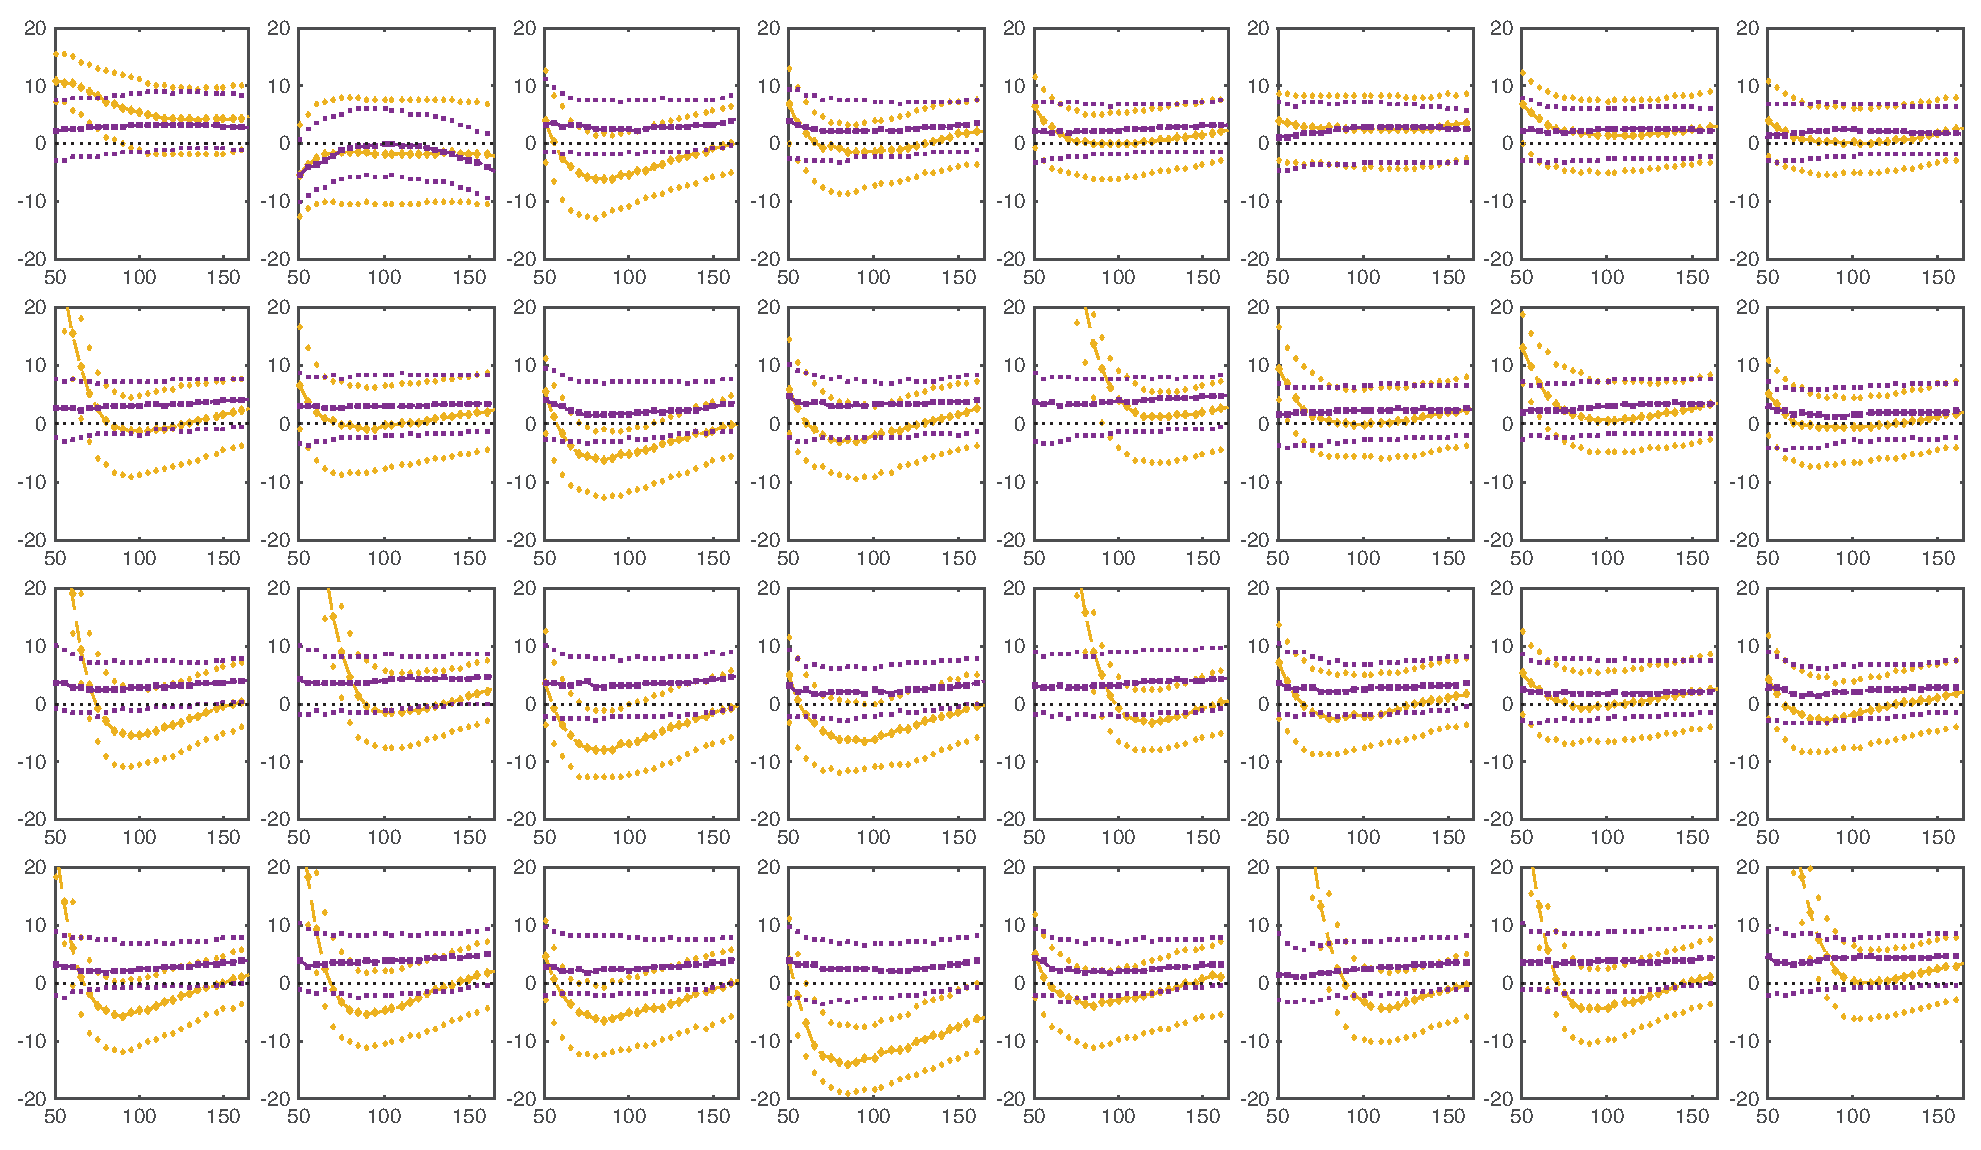
\includegraphics[width=0.95\linewidth]{simSamples_rF.eps}
        \caption{Median (large symbols) and first and third quartiles (small symbols) of the relative estimation error for the relative blood flow ($rF$) estimated using the \textbf{rLin} (yellow diamonds) and \textbf{rReg} (purple squares) models, as a function of the exam duration.}
        \label{fig:examDuration_rF}
    \end{figure}
    \begin{figure}\centering
        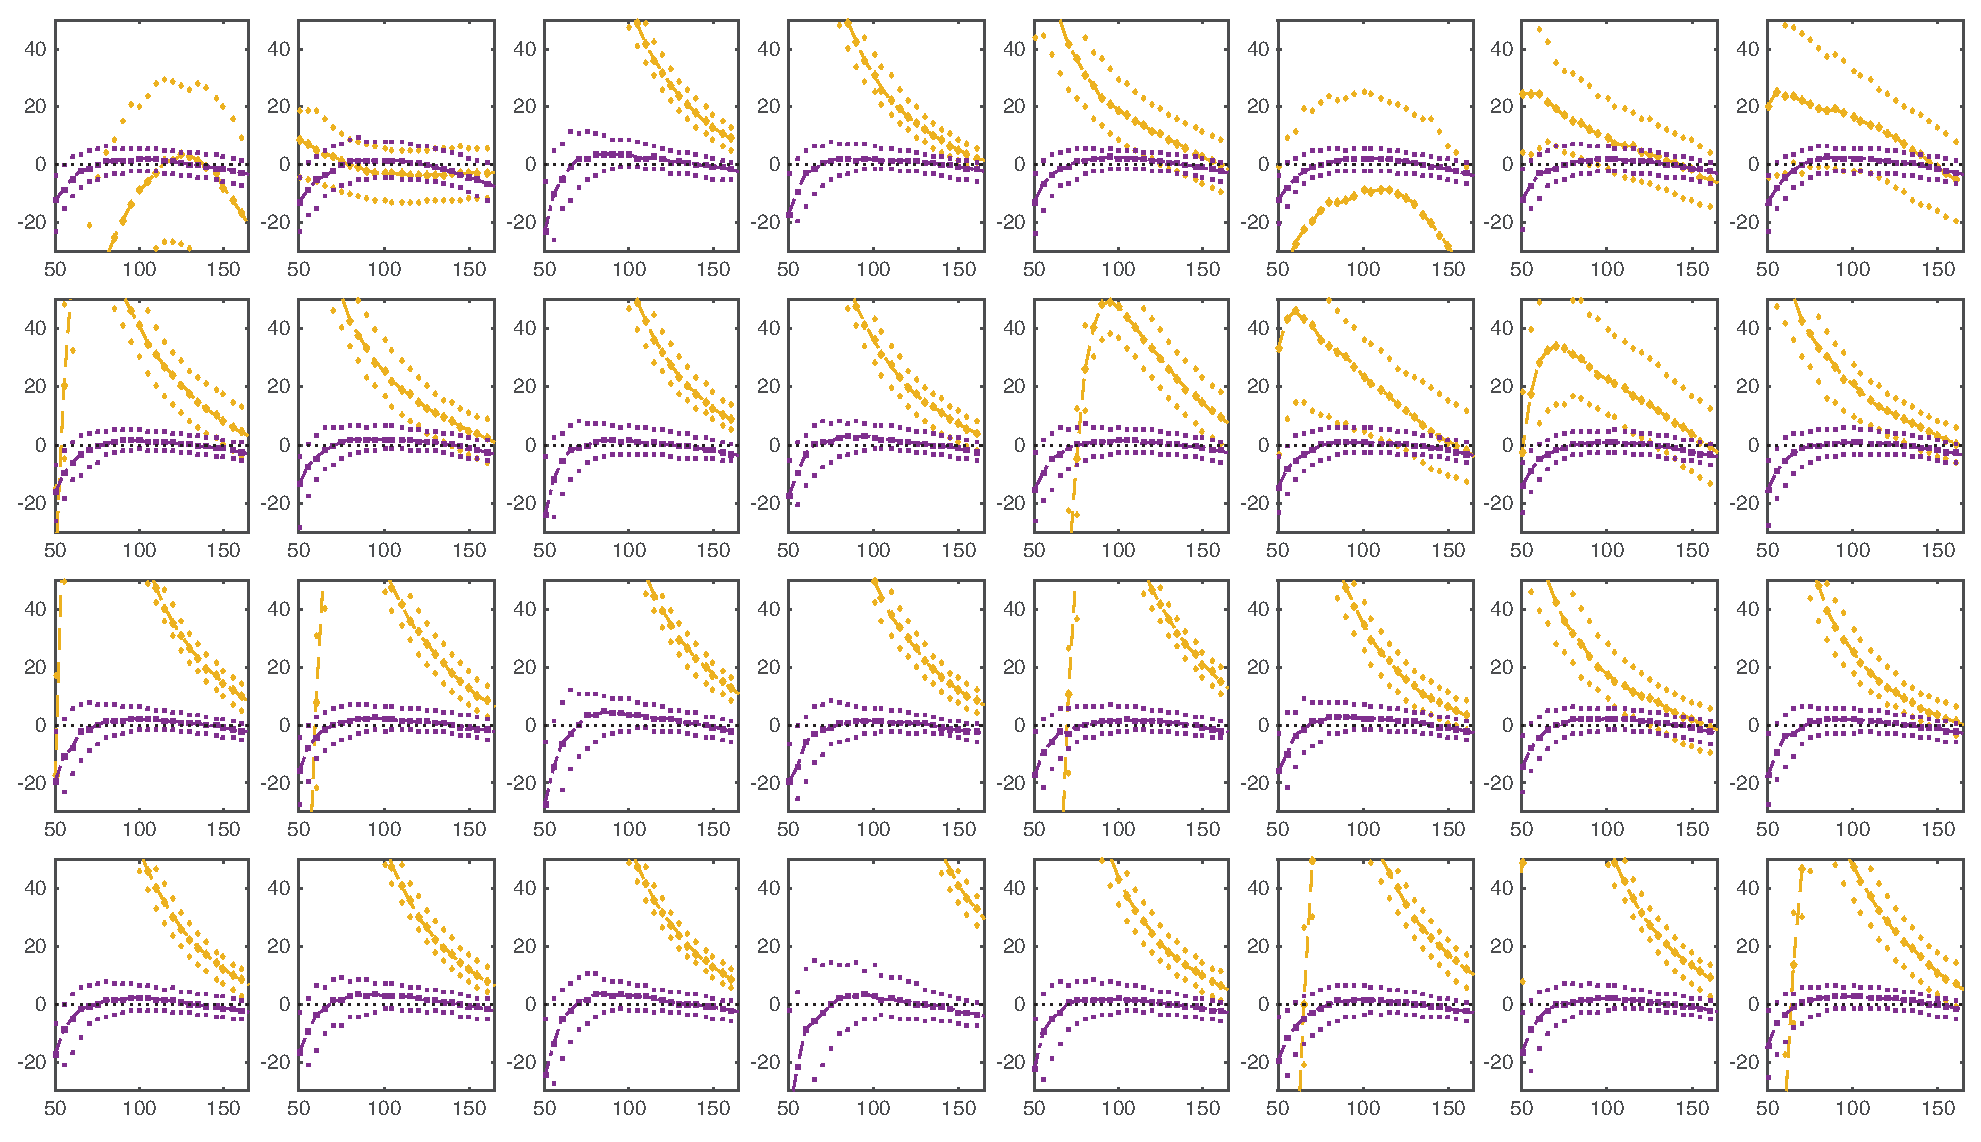
\includegraphics[width=0.95\linewidth]{simSamples_kT.eps}
        \caption{Median (large symbols) and first and third quartiles (small symbols) of the relative estimation error for the rate constant in the tumor ($k_T$) estimated using the \textbf{rLin} (yellow diamonds) and \textbf{rReg} (purple squares) models, as a function of the exam duration.}
        \label{fig:examDuration_kT}
    \end{figure}
    \begin{figure}\centering
        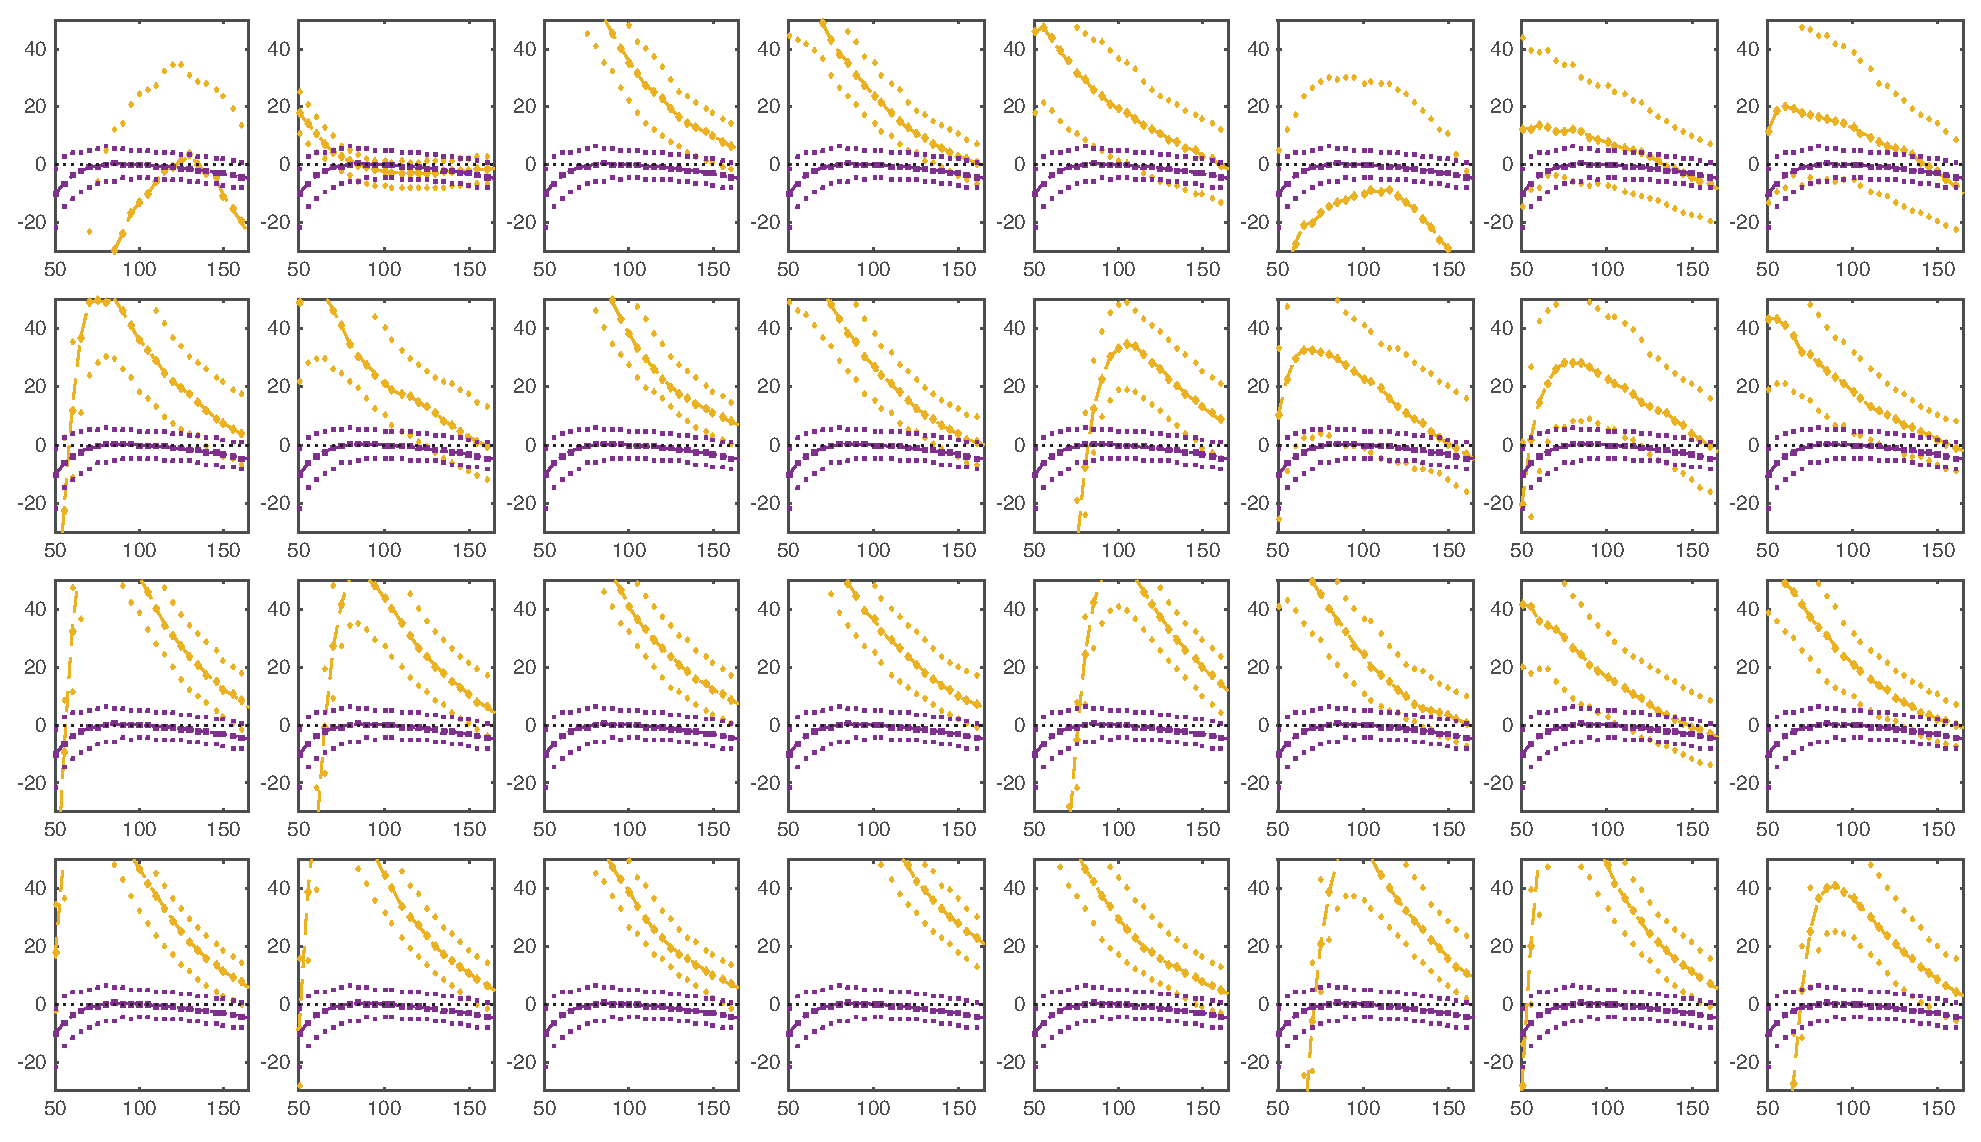
\includegraphics[width=0.95\linewidth]{simSamples_kR.eps}
        \caption{Median (large symbols) and first and third quartiles (small symbols) of the relative estimation error for the rate constant in the reference tissue ($k_R$) estimated using the \textbf{rLin} (yellow diamonds) and \textbf{rReg} (purple squares) models, as a function of the exam duration.}
        \label{fig:examDuration_kR}
    \end{figure}
\end{subfigures}
\FloatBarrier

\subsection{Sampling period}
Figures~\ref{fig:sampling_rV} to \ref{fig:sampling_kR} show the impact of the sampling period on the relative estimation error of the perfusion parameters of the \textbf{rLin} and \textbf{rReg} models, i.e.~relative tissue blood volume (Figure~\ref{fig:sampling_rV}), relative tissue blood flow (Figure~\ref{fig:sampling_rF}), and rate constants in the tumor (Figure~\ref{fig:sampling_kT}) and in the reference tissue (Figure~\ref{fig:sampling_kR}).

Varying the sampling period over the investigated range, i.e.~from 0.1 to 1 second, did not have a significant impact on the accuracy of the estimation of the relative tissue blood volume parameter using both the \textbf{rLin} and \textbf{rReg} models (see Figure~\ref{fig:sampling_rV}), and only a slight decrease in precision was observed for larger sampling period.
Similarly to the varying noise level experiments, the bias in the estimation bias of $rV$ was more consistent across regions using the \textbf{rReg} model, with the median relative estimation errors generally inferior to 4\%.
The estimates of $rF$, the relative tissue blood flow, exhibited a tendency to decrease with increasing sampling period, especially in regions with large simulated $k_T$ values. 
While in most regions the estimates of $rF$ from the \textbf{rReg} model get closer to zero for large sampling periods, one region underestimated the parameter by more than 20\%.
The estimates of $rF$ from the \textbf{rLin} model exhibited a similar trend, but in addition they were overall more sensitive to the sampling period in terms of precision, and less consistent across regions.
In terms of rate constant in the tumor (see Figure~\ref{fig:sampling_kT}), the \textbf{rReg} model yielded consistent negative biases across regions, and generally yielded more precise estimates than the \textbf{rLin} model.
For both models, a slight decrease of the estimates of $k_T$ with the sampling period was observed for both models in most regions, but stronger negative slopes were observed in regions with larger simulated $k_T$.
The rate constant in the reference tissue was estimated consistently across tumor regions using the \textbf{rReg} model (see Figure~\ref{fig:sampling_kR}), and the estimation was overall more accurate and precise with this model.
Indeed, the estimation of $k_R$ using the \textbf{rLin} model was extremely imprecise in some regions.

\begin{subfigures}
    \begin{figure}
        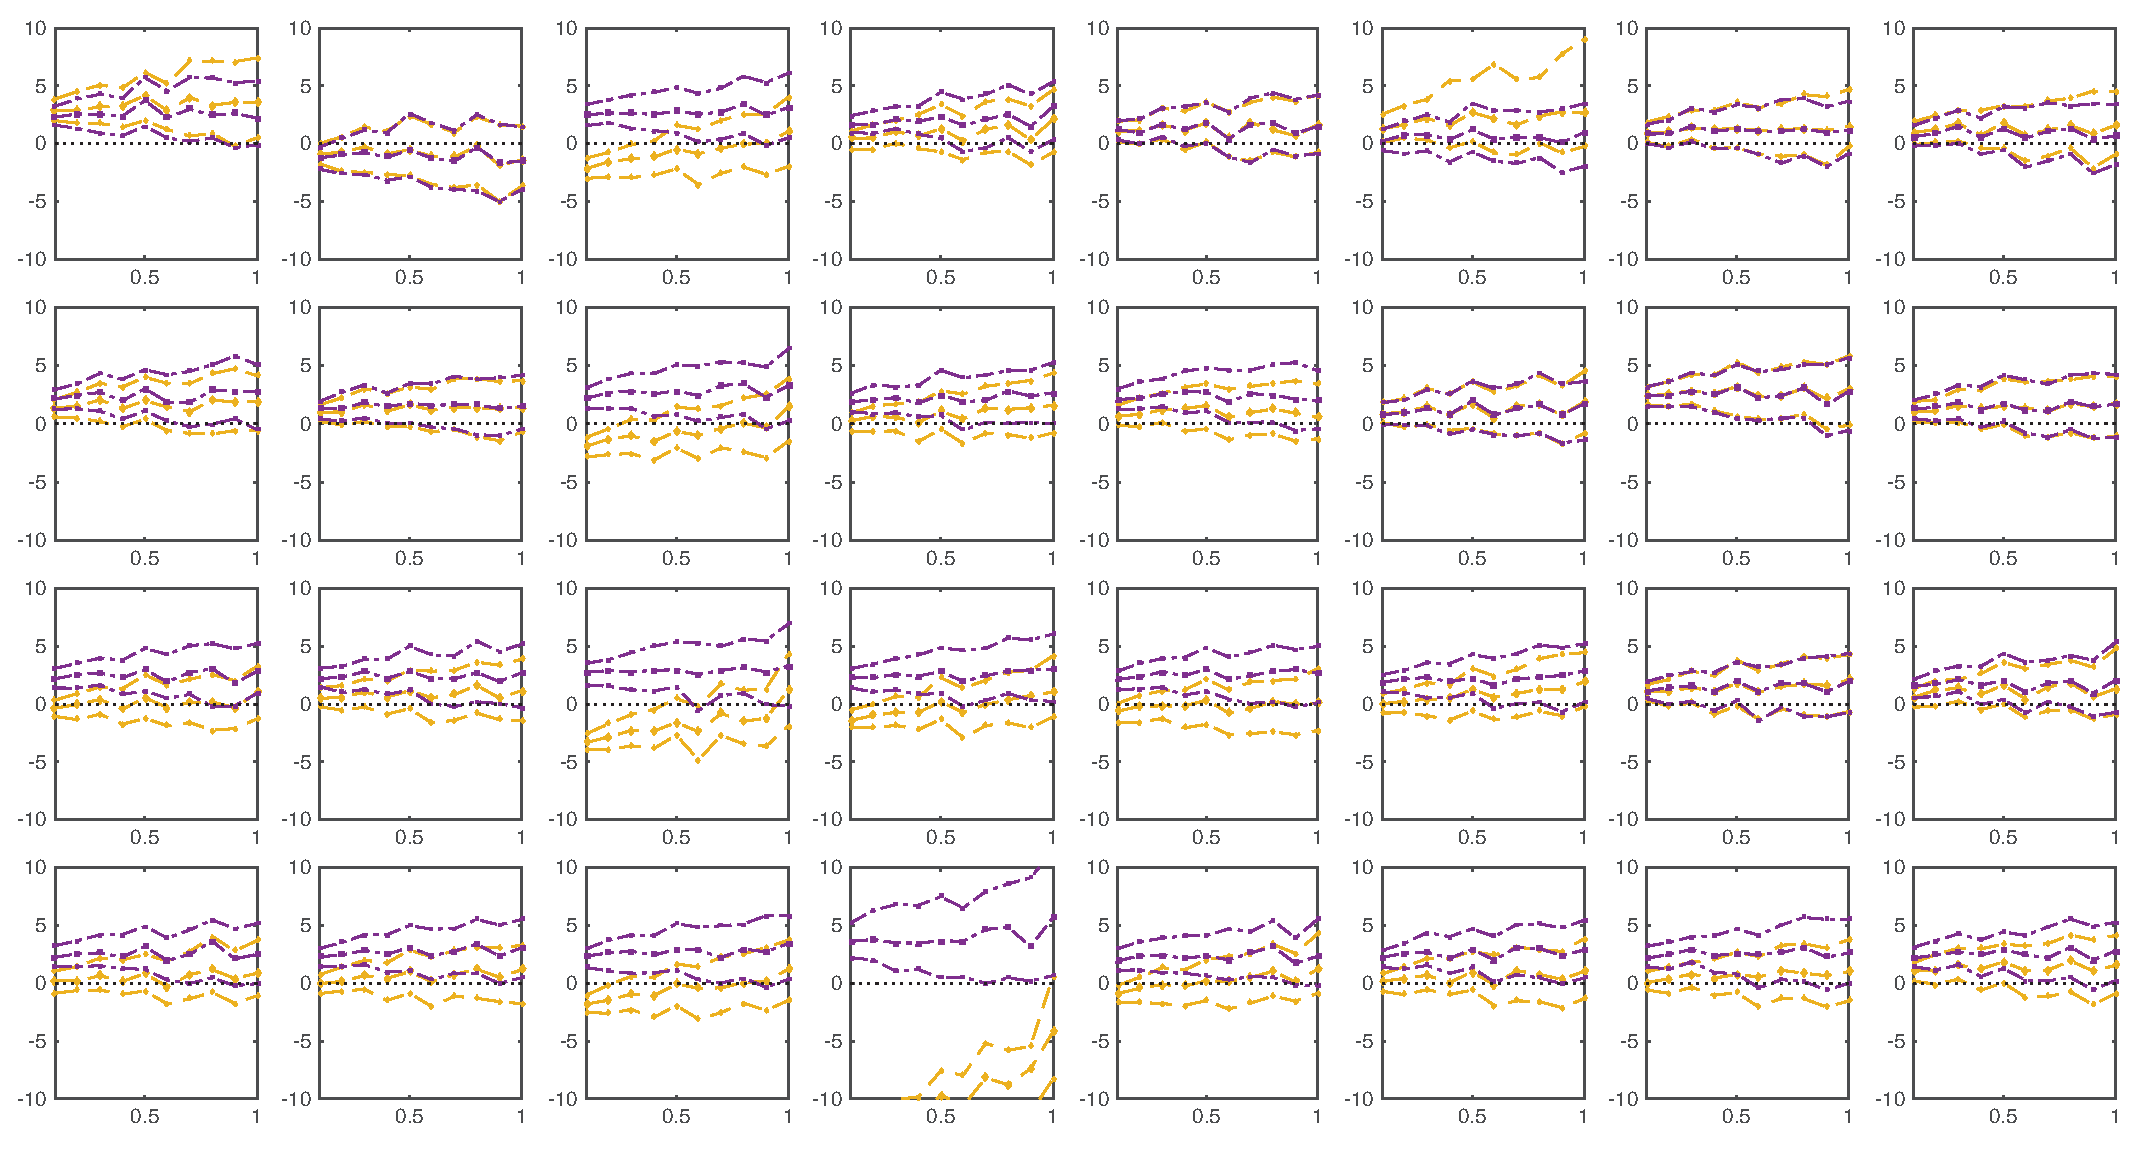
\includegraphics[width=\linewidth]{simSampling_rV.eps}
        \caption{Median (large symbols) and first and third quartiles (small symbols) of the relative estimation error for the relative tissue blood volume ($rV$) estimated using the \textbf{rLin} (yellow diamonds) and \textbf{rReg} (purple squares) models, depending on the sampling period used for simulation.}
        \label{fig:sampling_rV}
    \end{figure}
    \begin{figure}
        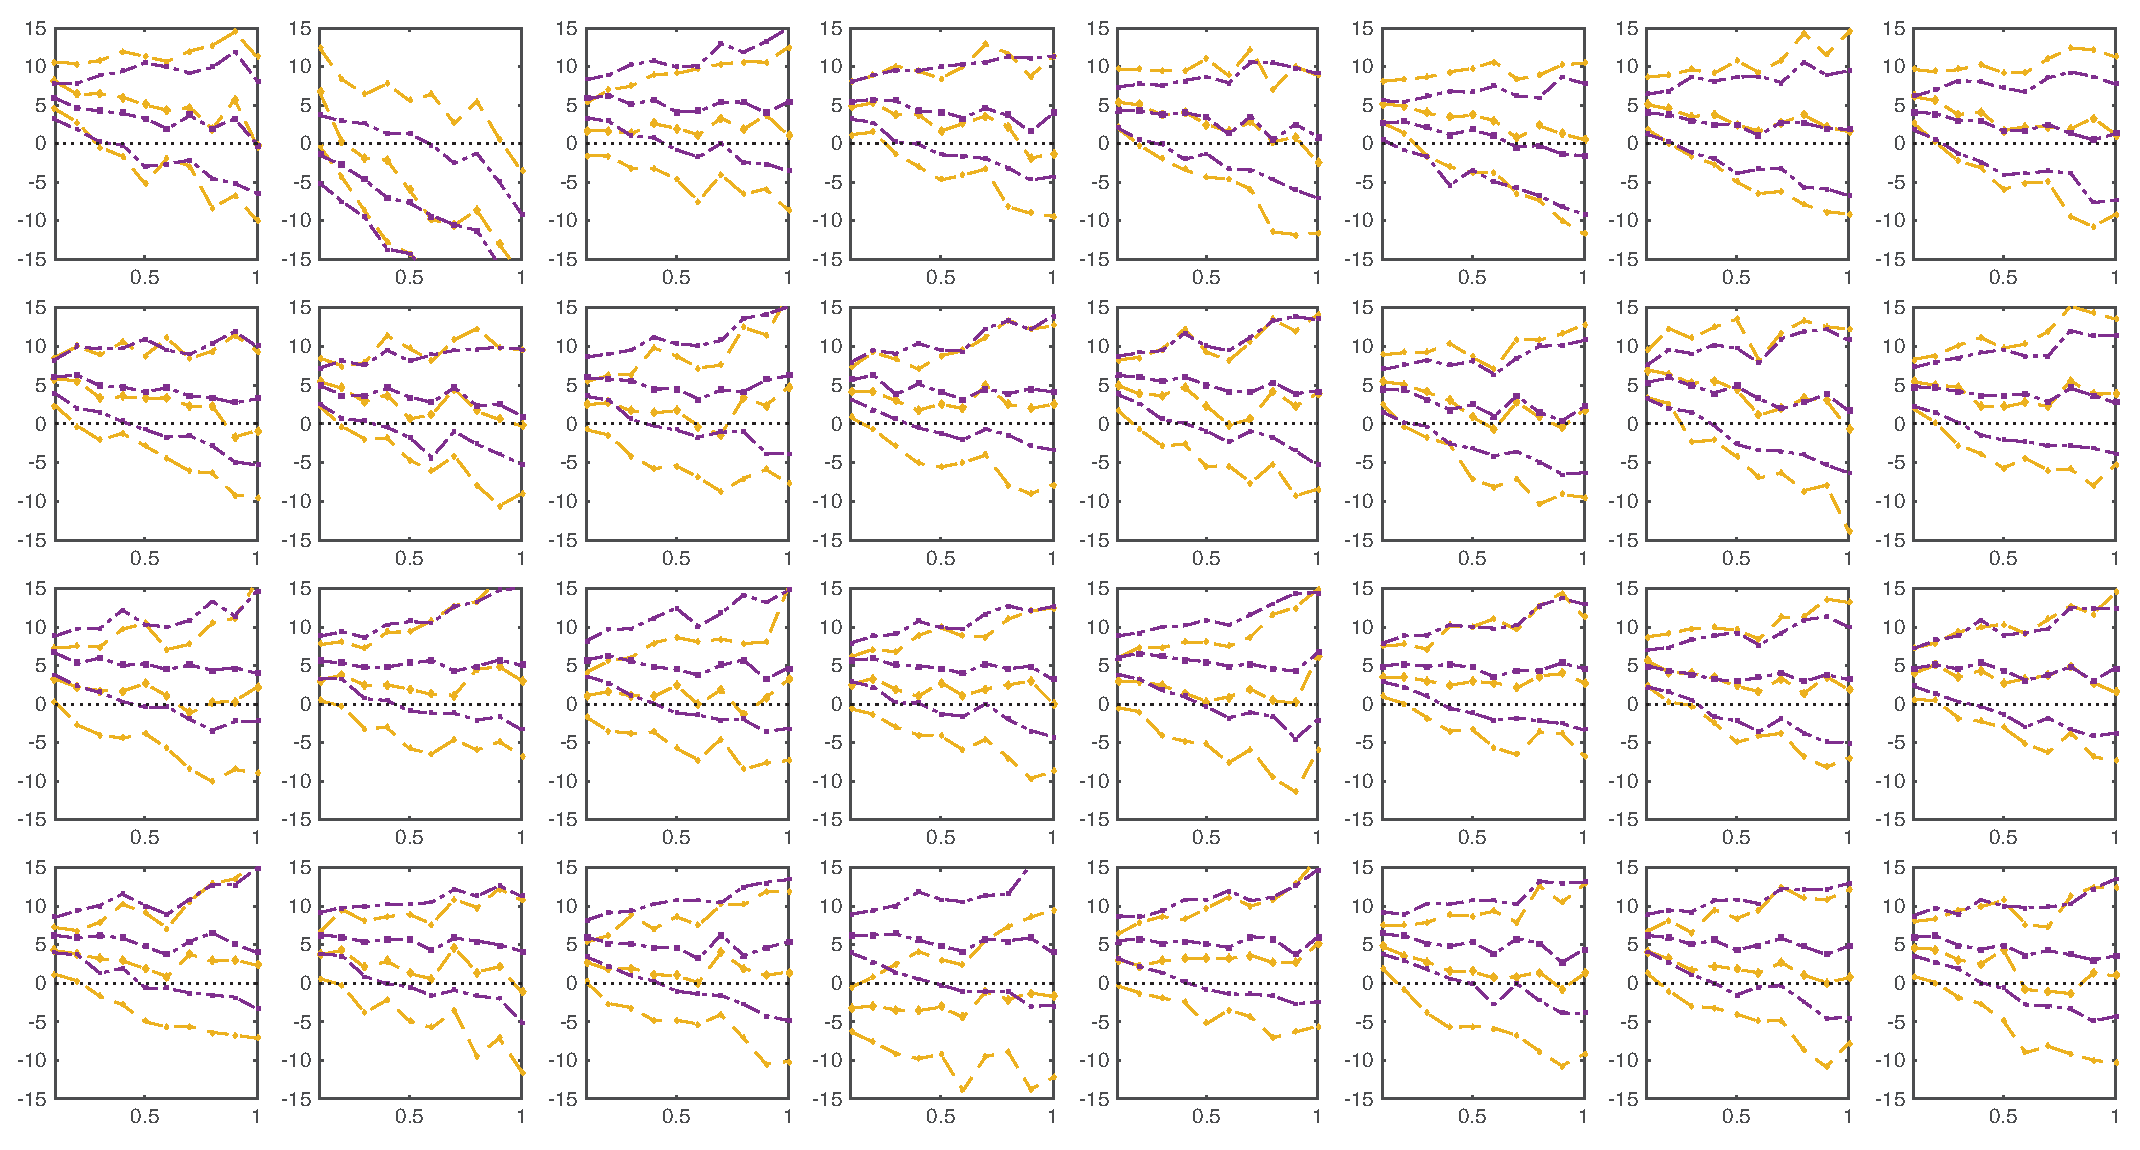
\includegraphics[width=\linewidth]{simSampling_rF.eps}
        \caption{Median (large symbols) and first and third quartiles (small symbols) of the relative estimation error for the relative tissue blood flow ($rF$) estimated using the \textbf{rLin} (yellow diamonds) and \textbf{rReg} (purple squares) models, depending on the sampling period used for simulation.}
        \label{fig:sampling_rF}
    \end{figure}
    \begin{figure}
        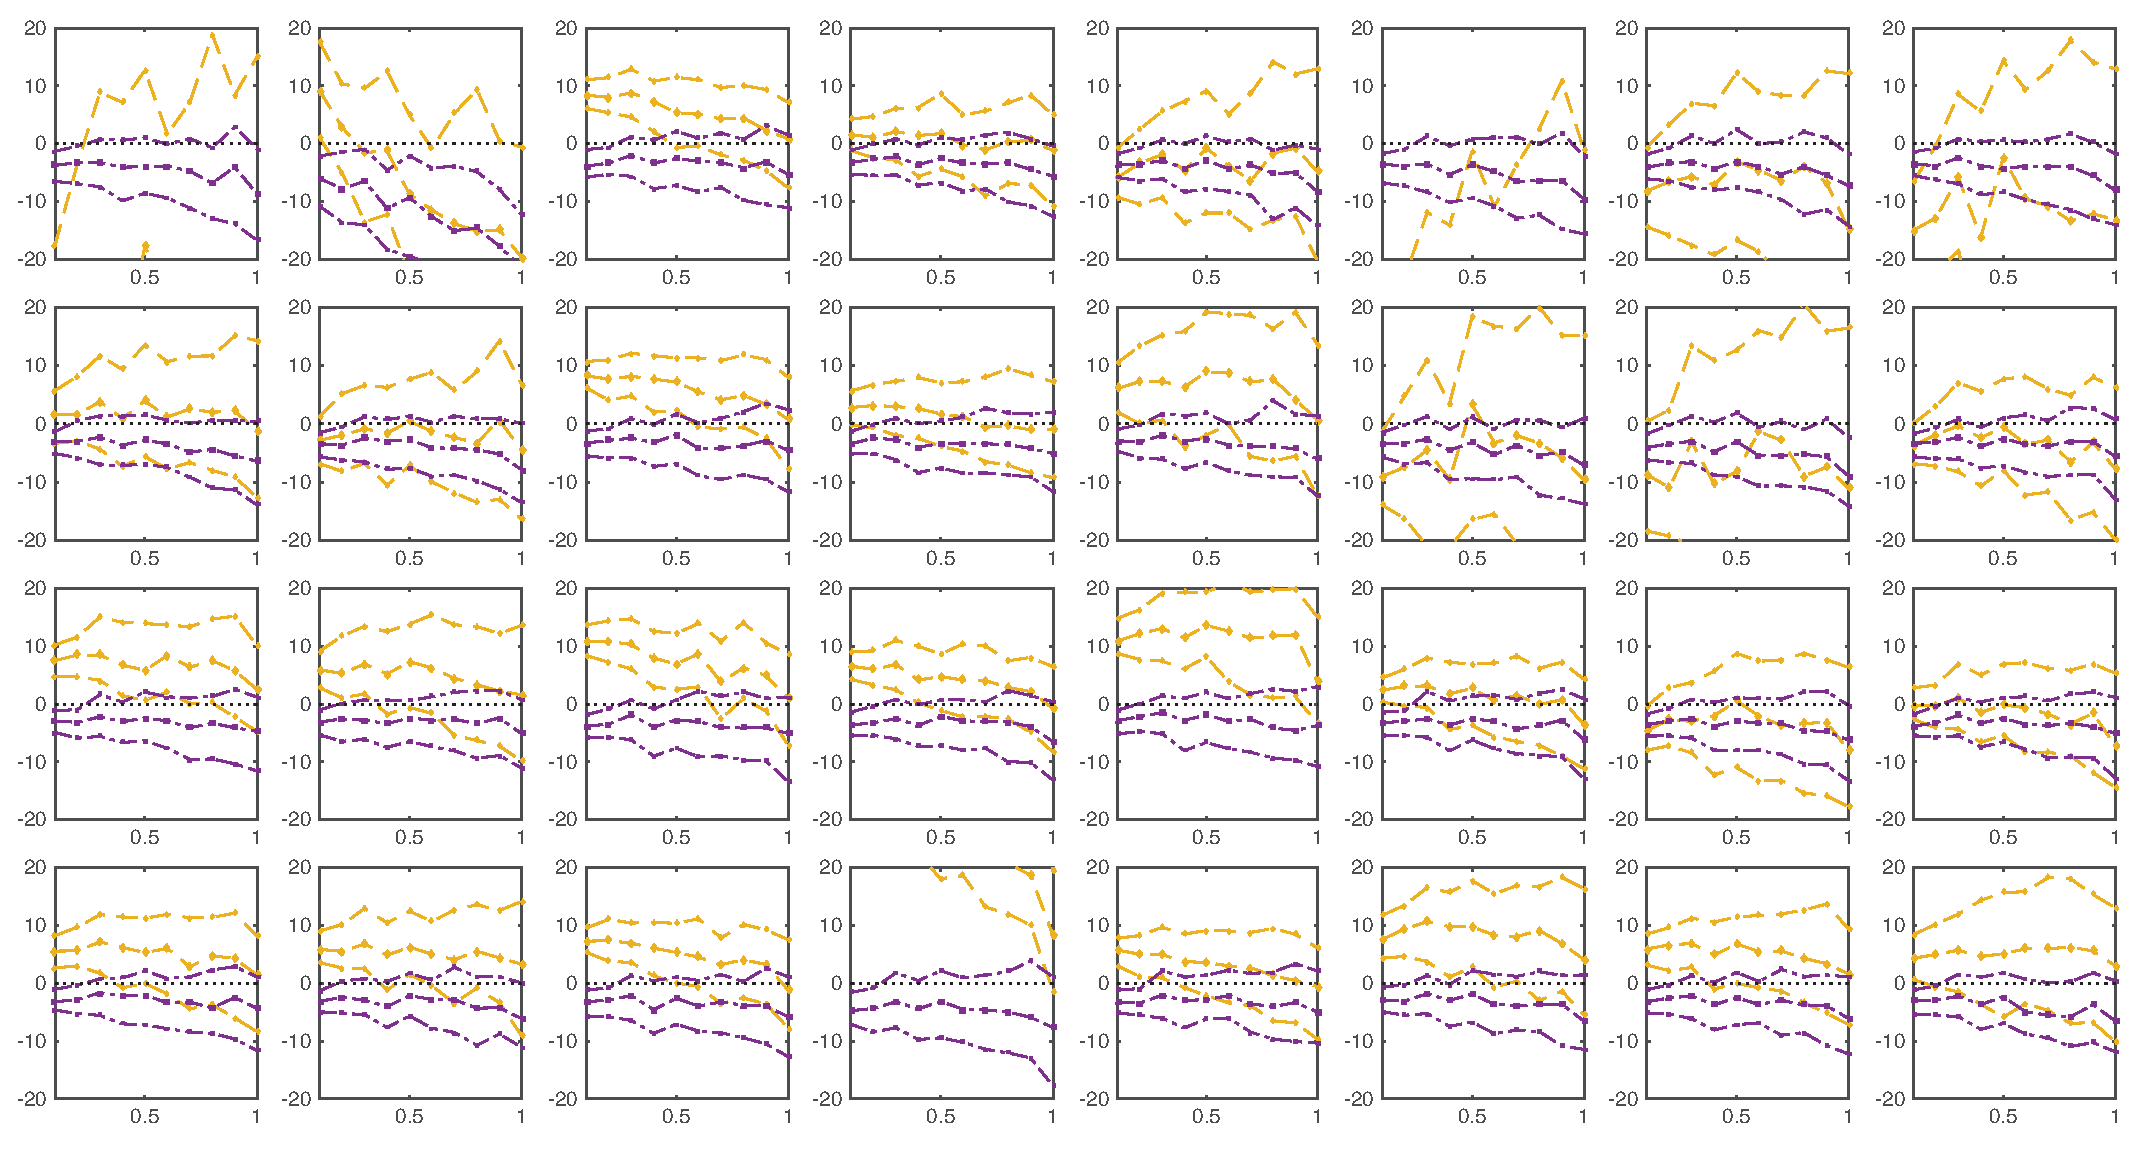
\includegraphics[width=\linewidth]{simSampling_kT.eps}
        \caption{Median (large symbols) and first and third quartiles (small symbols) of the relative estimation error for the rate constant in the tumor ($k_T$) estimated using the \textbf{rLin} (yellow diamonds) and \textbf{rReg} (purple squares) models, depending on the sampling period used for simulation.}
        \label{fig:sampling_kT}
    \end{figure}
    \begin{figure}
        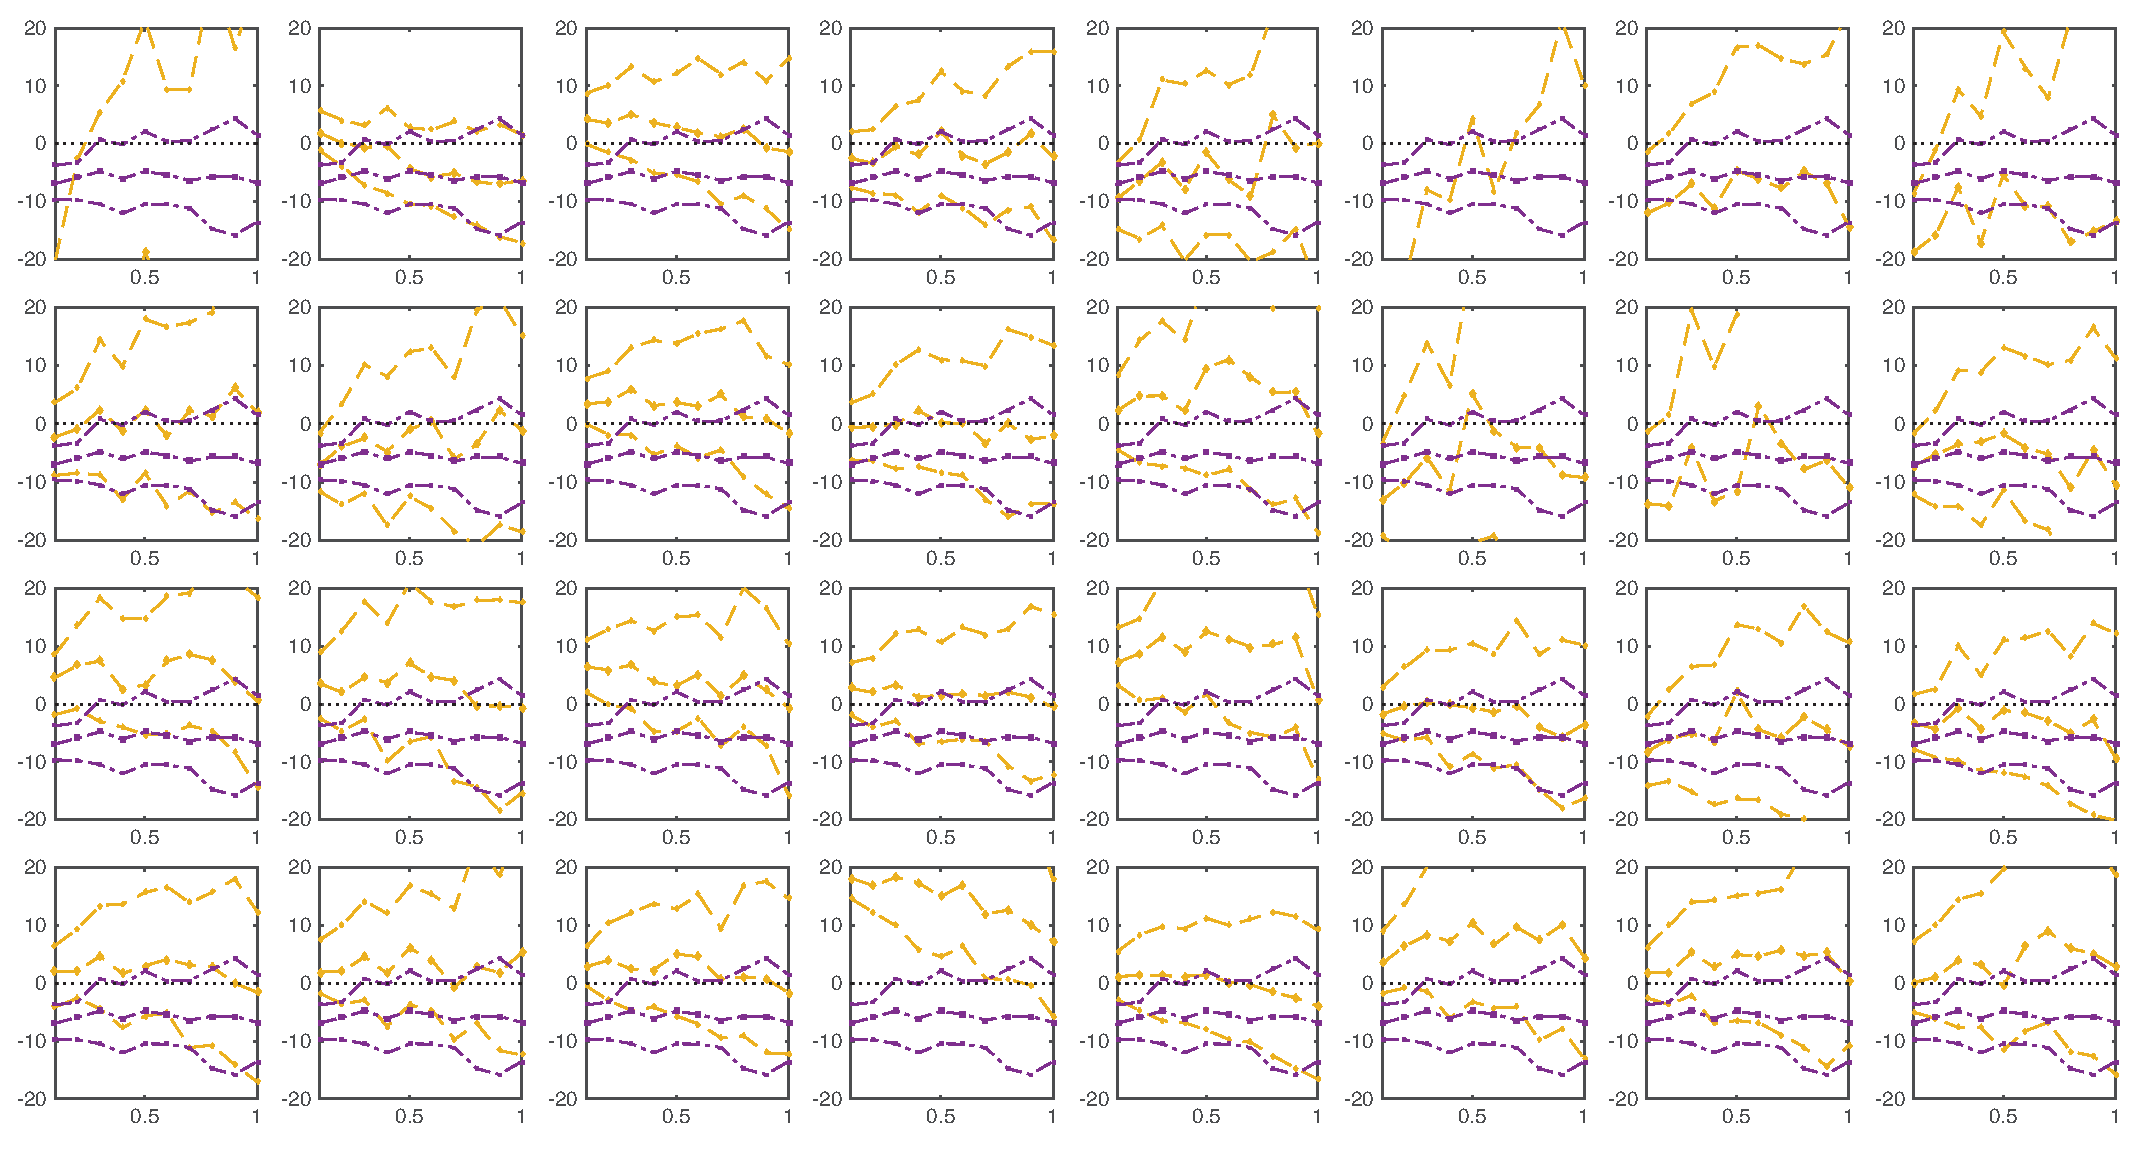
\includegraphics[width=\linewidth]{simSampling_kR.eps}
        \caption{Median (large symbols) and first and third quartiles (small symbols) of the relative estimation error for the rate constant in the reference tissue ($k_R$) estimated using the \textbf{rLin} (yellow diamonds) and \textbf{rReg} (purple squares) models, depending on the sampling period used for simulation.}
        \label{fig:sampling_kR}
    \end{figure}
\end{subfigures}
\FloatBarrier

\subsection{Reference tissue}
The effect of varying the characteristics of the reference tissue on the accuracy and precision of the estimation process are displayed in Figures~\ref{fig:referenceTissue_rV} to~\ref{fig:referenceTissue_kR}. 
In any of these four Figures, the first and fourth lines correspond to fixed values of the tissue blood volume $V_R$ with varying tissue blood flow $F_R$, the second and fifth lines correspond to fixed values of $F_R$ with varying $V_R$, and the third and sixth lines correspond to fixed values of $k_R$ with varying values of both $V_R$ and $F_R$.
Each bullseye displays the median relative estimation error in each of the 32 tumor regions for the considered parameter.

The relative tissue blood volume (see Figure~\ref{fig:referenceTissue_rV}), $rV$, estimated using the \textbf{rLin} model revealed sensitive to variations of parameter $k_R$.
Indeed, an increase in $k_R$ resulted in increased positive or negative biases, along with increased heterogeneity of the bias across regions.
Using the \textbf{rReg} model reduced the discrepancies across regions compared to the \textbf{rLin} model, but varying $k_R$ one way or the other overestimated the values of $rV$.
Similarly, the relative blood flow (see Figure~\ref{fig:referenceTissue_rF}), $rF$, estimated using either the \textbf{rLin} model or the \textbf{rReg} model were sensitive to variations of $k_R$. 
Larger biases were found using the \textbf{rReg} model, however larger discrepancies across regions were observed in the estimation biases of the \textbf{rLin} model.
For both models, $rF$ was underestimated in regions with large simulated $k_T$, while the other regions were overestimated.
The smallest biases in the estimation of $rF$ were found for two thirds of the original $k_R$ value.
In case of fixed $k_R$ values, using lower values of both $F_R$ and $V_R$ yielded slightly overestimated $rV$ and $rF$ values using both models.
Regarding the rate constant in the tumor (see Figure~\ref{fig:referenceTissue_kT}), $k_T$, large discrepancies can be observed using the \textbf{rLin} model, and they tend to increase with decreasing values of $k_R$.
Using the \textbf{rReg} model, the bias in the estimation of $k_T$ increased for lower values of $k_R$.
Additionally, discrepancies across regions are almost inexistant using the \textbf{rReg} model, except in regions with large simulated $k_T$ values, revealing the effect of regularization.
Biases close to zero were found in most regions simulating the reference tissue curve using two thirds of the original $k_R$ value.
The rate constant in the reference tissue (see Figure~\ref{fig:referenceTissue_kR}), $k_R$, exhibited behaviors extremely similar to those of $k_T$, whether estimated using the \textbf{rLin} model or the \textbf{rReg} model.
In case of fixed $k_R$ values, using lower values of both $F_R$ and $V_R$ yielded slightly underestimated $kT$ and $kR$ values using both models.

\begin{subfigures}
    \begin{figure}
        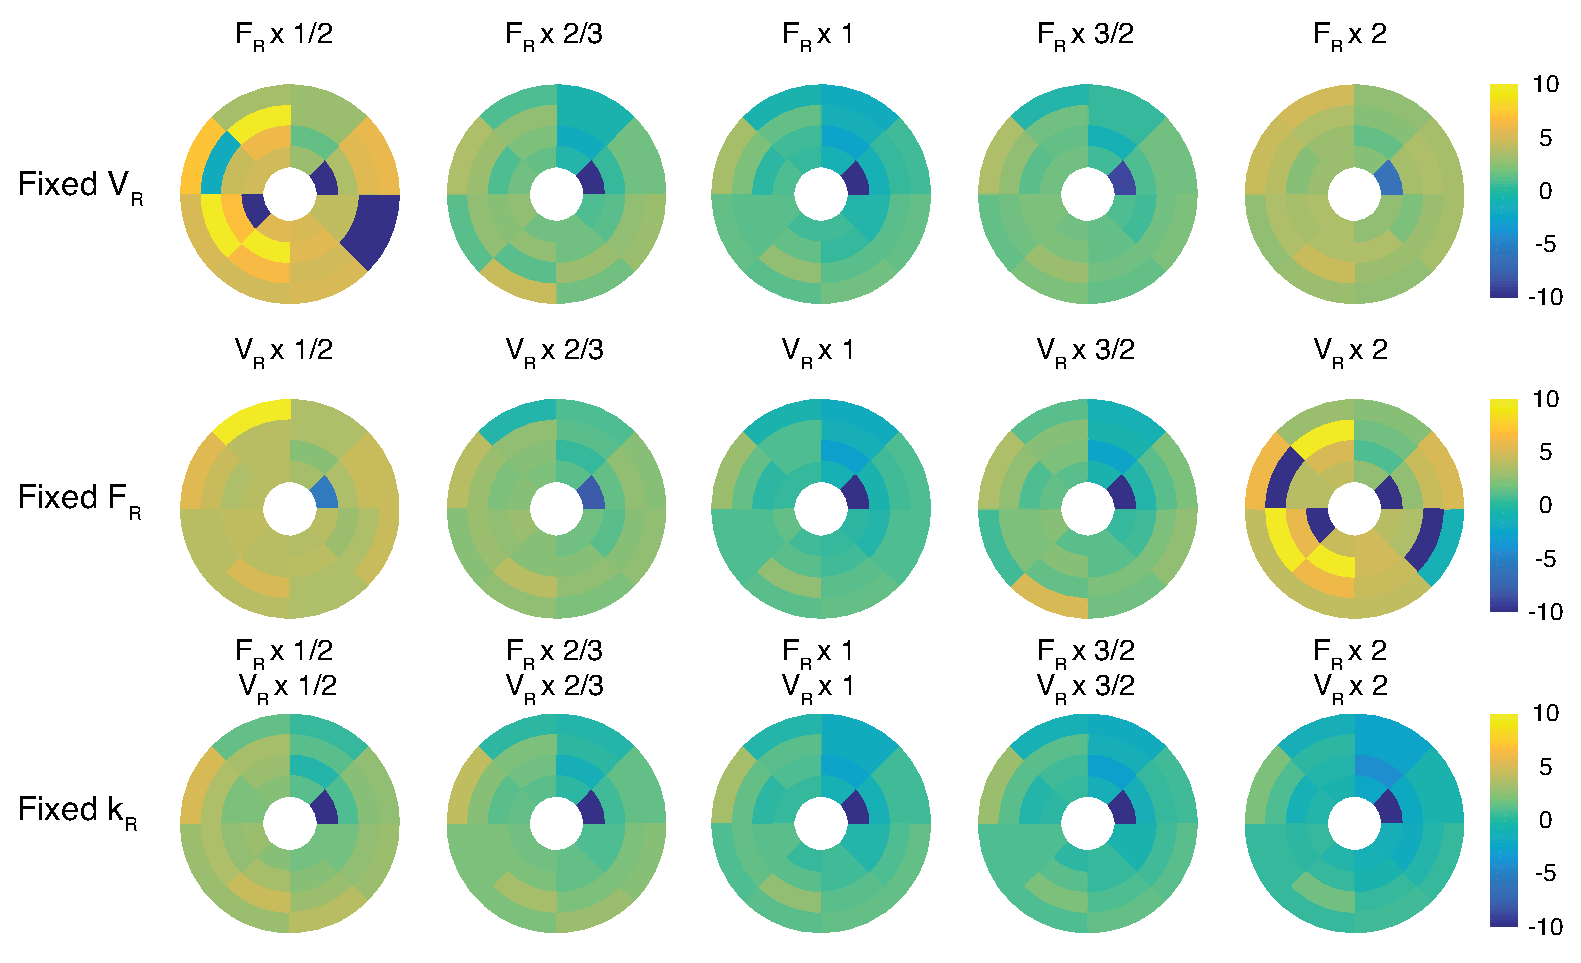
\includegraphics[width=\linewidth]{simRef_rV_rLin.eps}
        \par\vspace{1cm}
        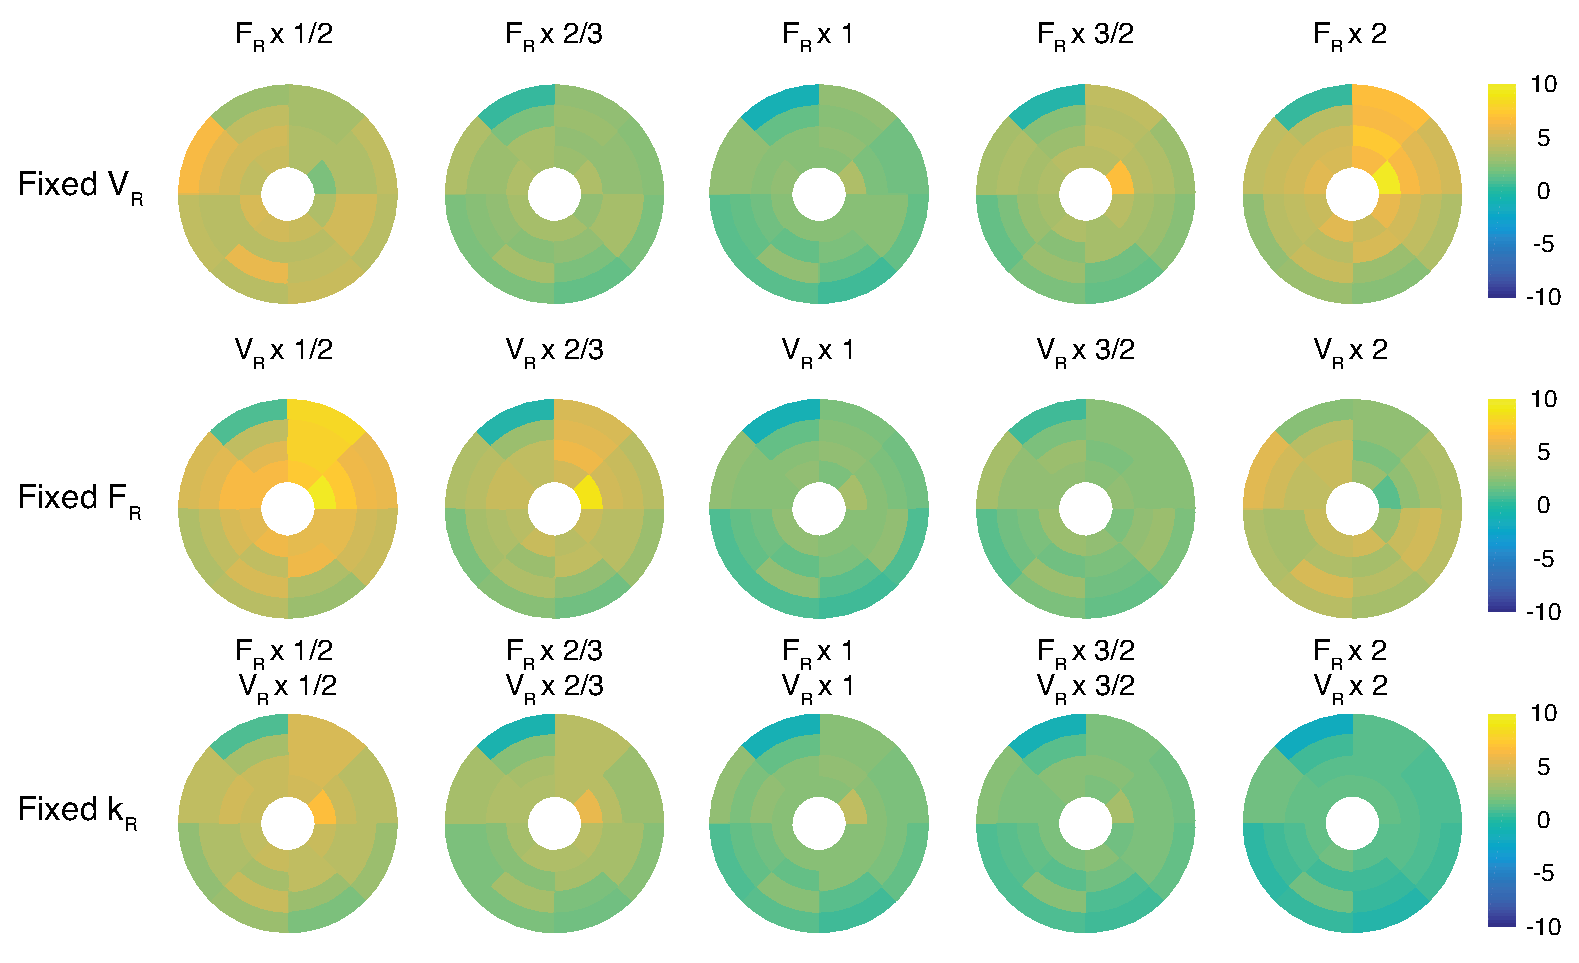
\includegraphics[width=\linewidth]{simRef_rV_rReg.eps}
        \caption{Bullseyes of the median relative estimation error for the relative tissue blood volume ($rV$) estimated using the \textbf{rLin} (top) and \textbf{rReg} (bottom) models depending on the characteristics of the reference tissue used for simulation.}
        \label{fig:referenceTissue_rV}
    \end{figure}
    \begin{figure}
        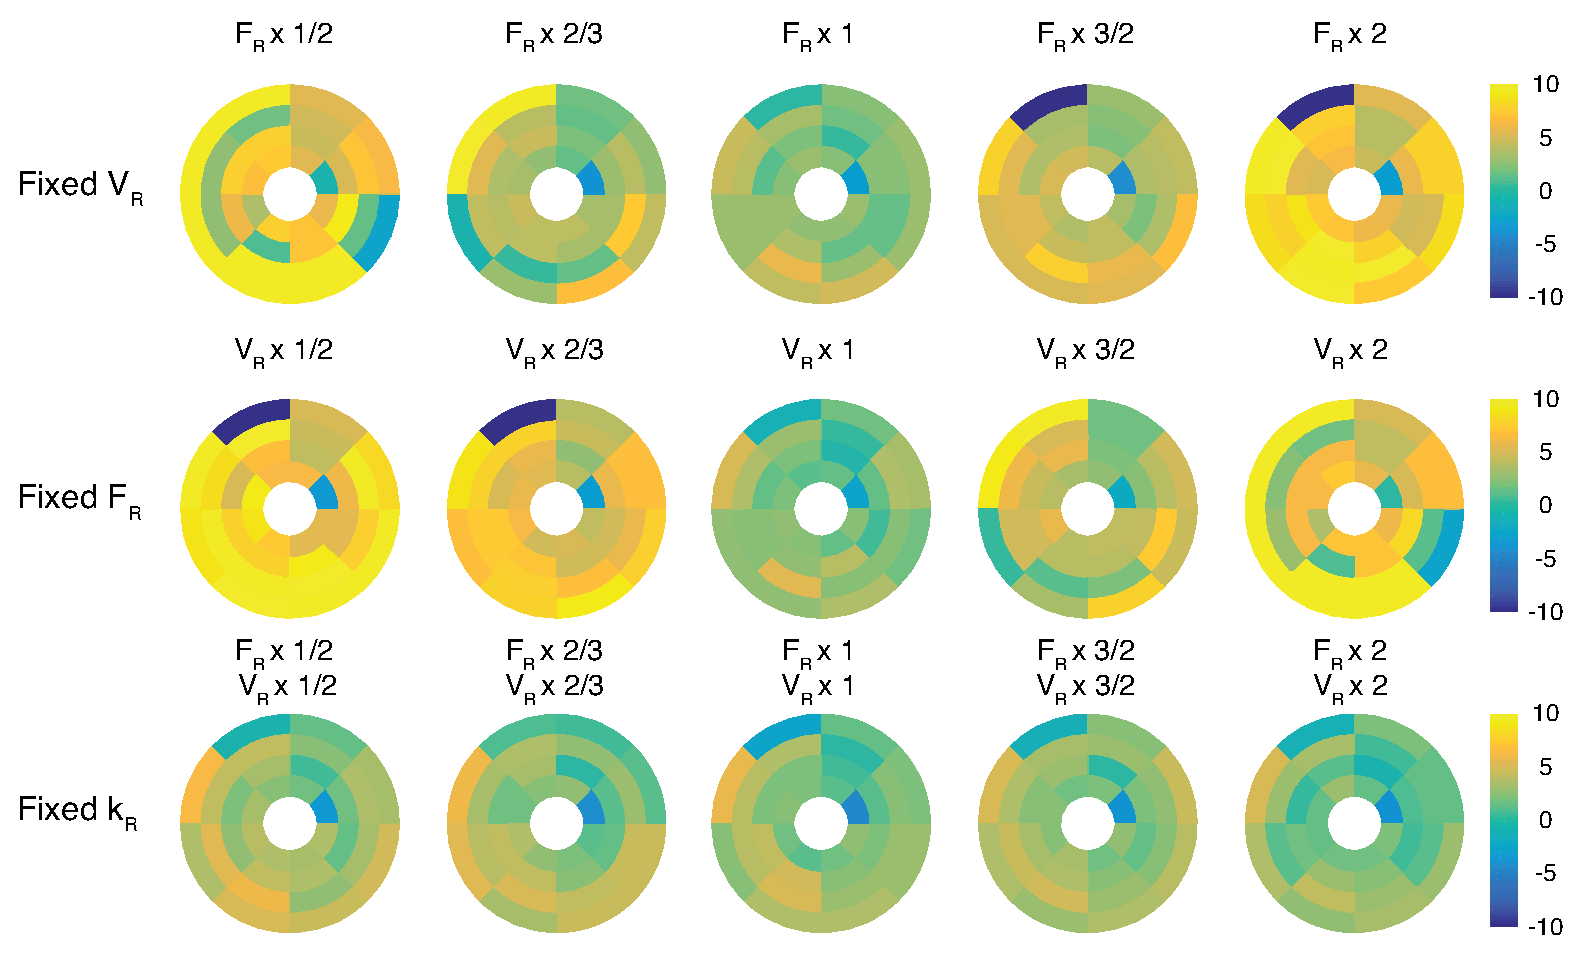
\includegraphics[width=\linewidth]{simRef_rF_rLin.eps}
        \par\vspace{1cm}
        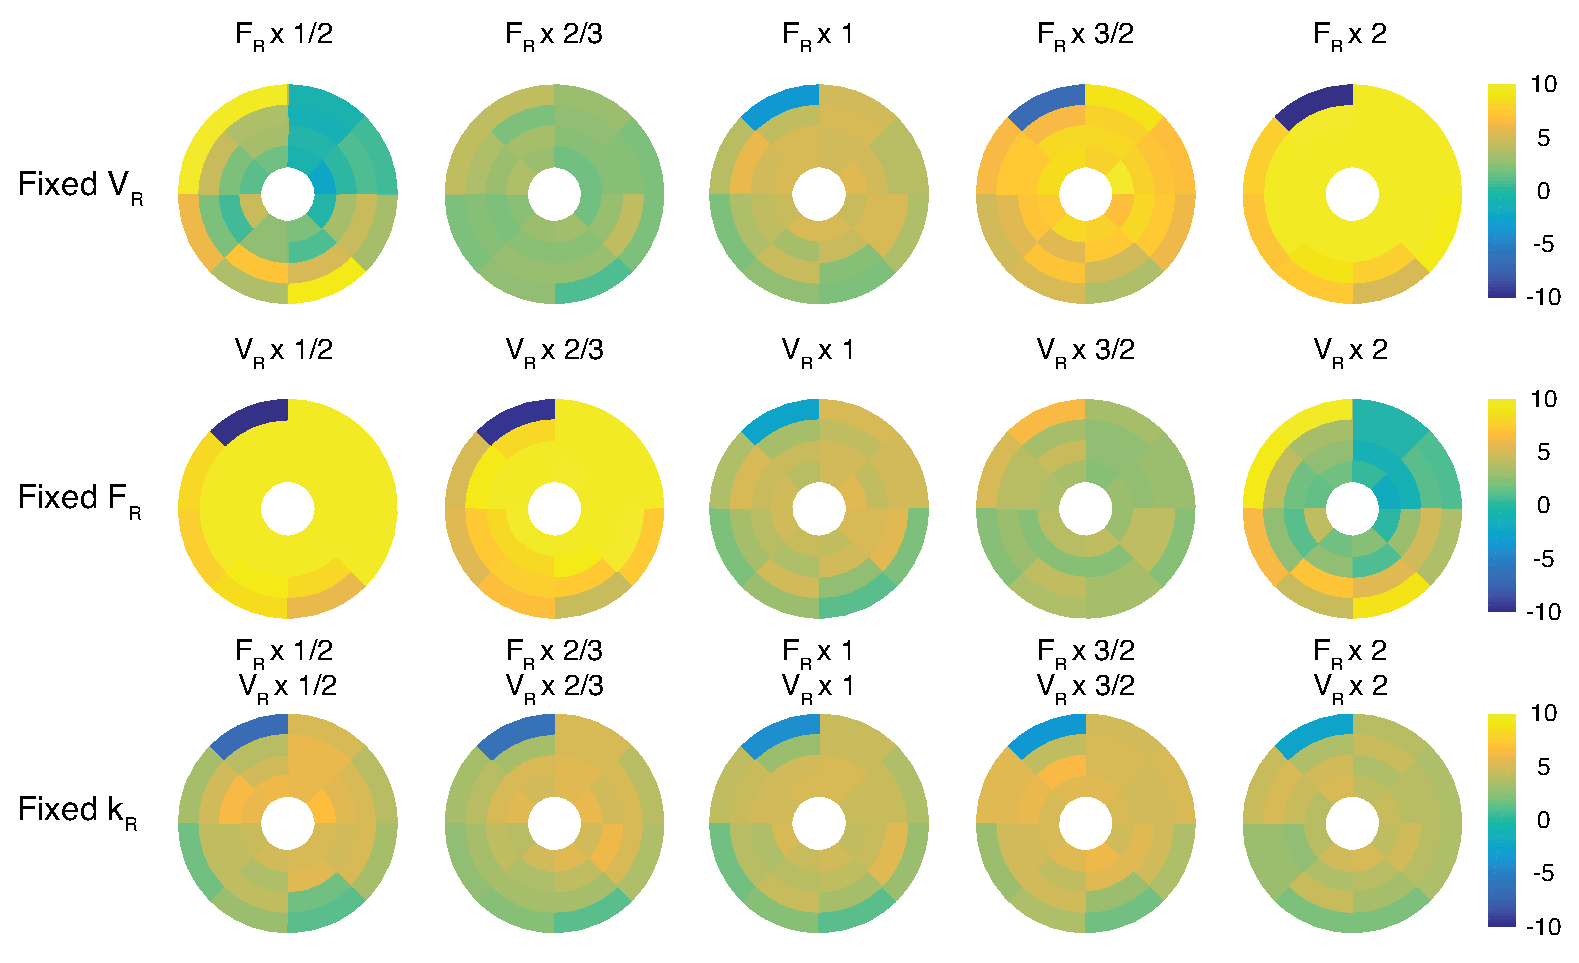
\includegraphics[width=\linewidth]{simRef_rF_rReg.eps}
        \caption{Bullseyes of the median relative estimation error for the relative tissue blood flow ($rF$) estimated using the \textbf{rLin} (top) and \textbf{rReg} (bottom) models depending on the characteristics of the reference tissue used for simulation.}
        \label{fig:referenceTissue_rF}
    \end{figure}
    \begin{figure}
        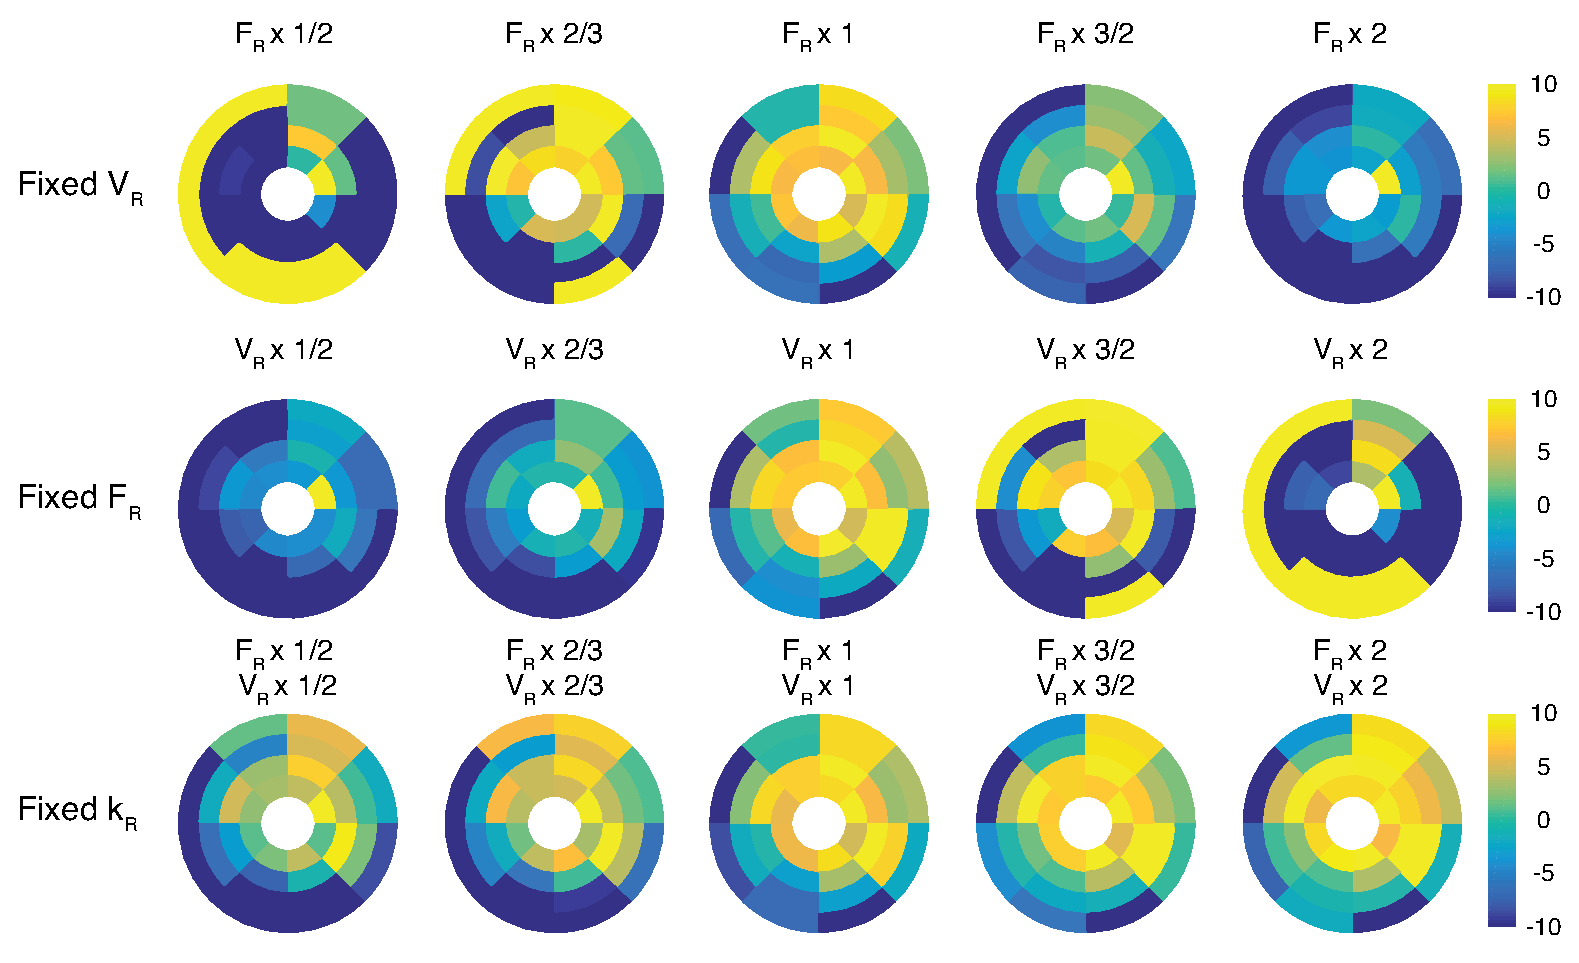
\includegraphics[width=\linewidth]{simRef_kT_rLin.eps}
        \par\vspace{1cm}
        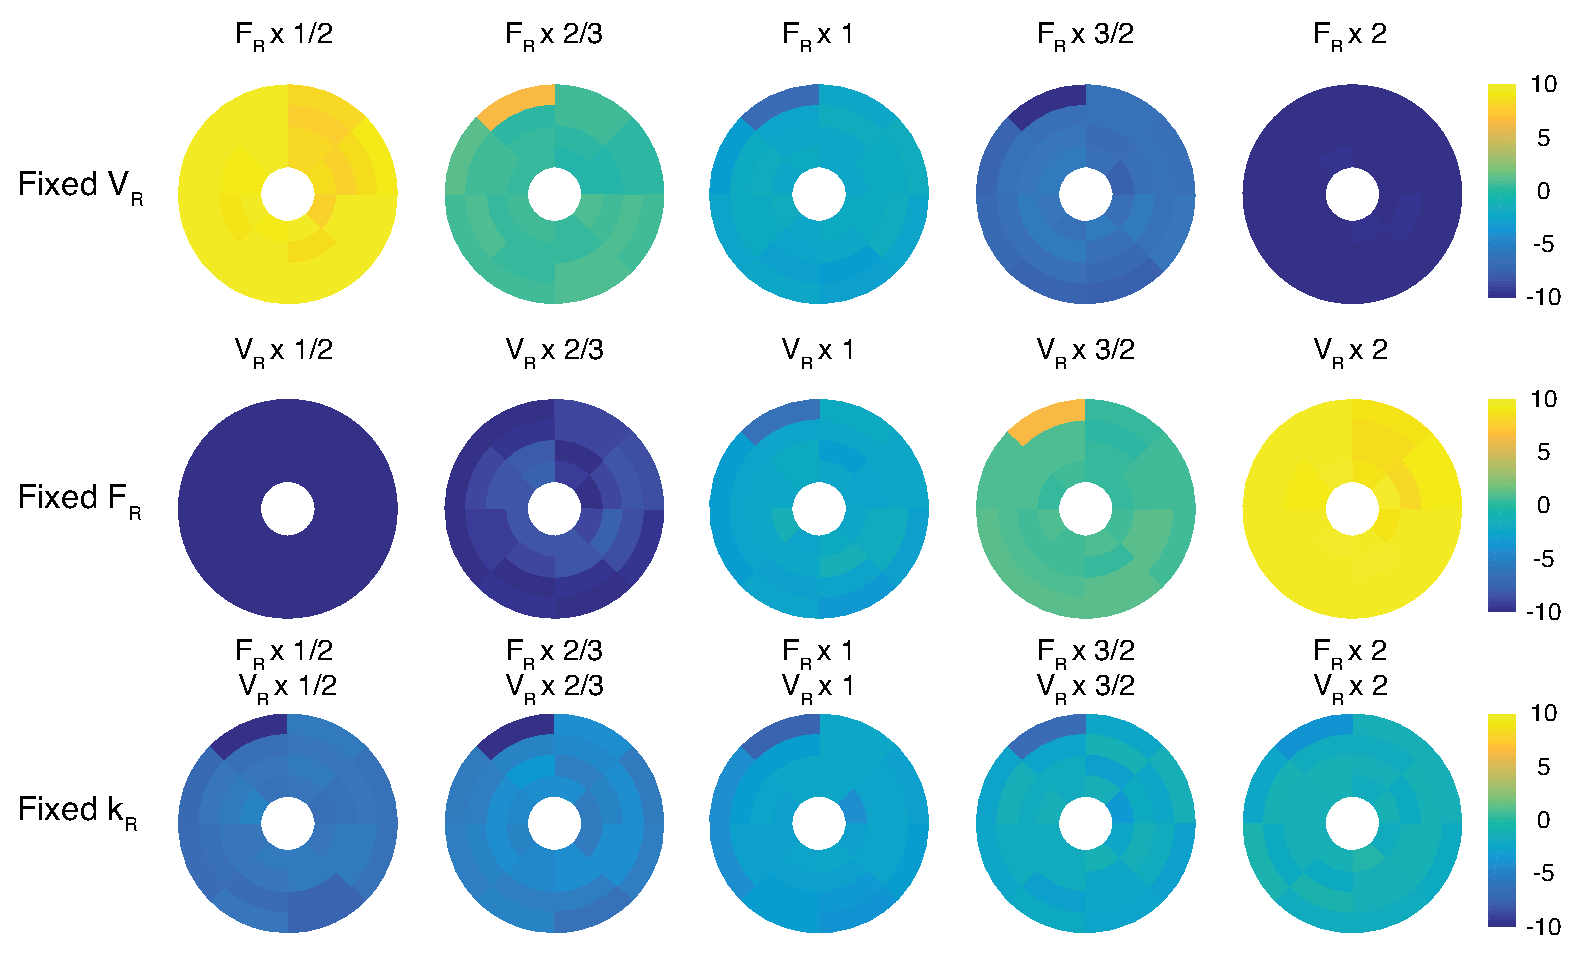
\includegraphics[width=\linewidth]{simRef_kT_rReg.eps}
        \caption{Bullseyes of the median relative estimation error for the rate constant in the tumor ($k_T$) estimated using the \textbf{rLin} (top) and \textbf{rReg} (bottom) models depending on the characteristics of the reference tissue used for simulation.}
        \label{fig:referenceTissue_kT}
    \end{figure}
    \begin{figure}
        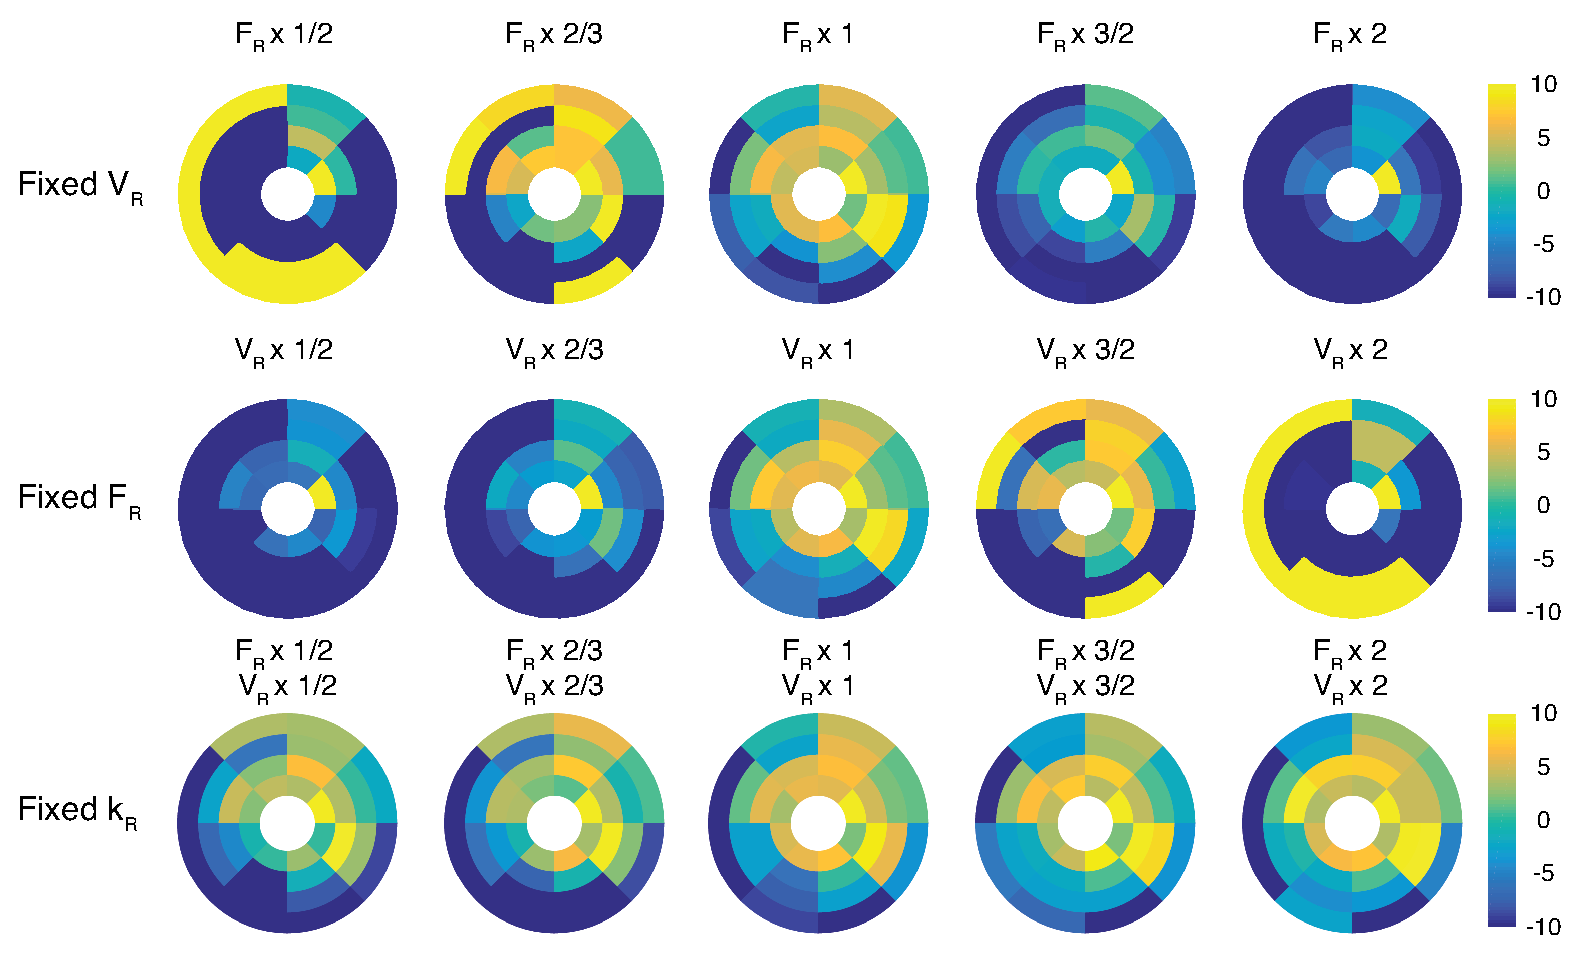
\includegraphics[width=\linewidth]{simRef_kR_rLin.eps}
        \par\vspace{1cm}
        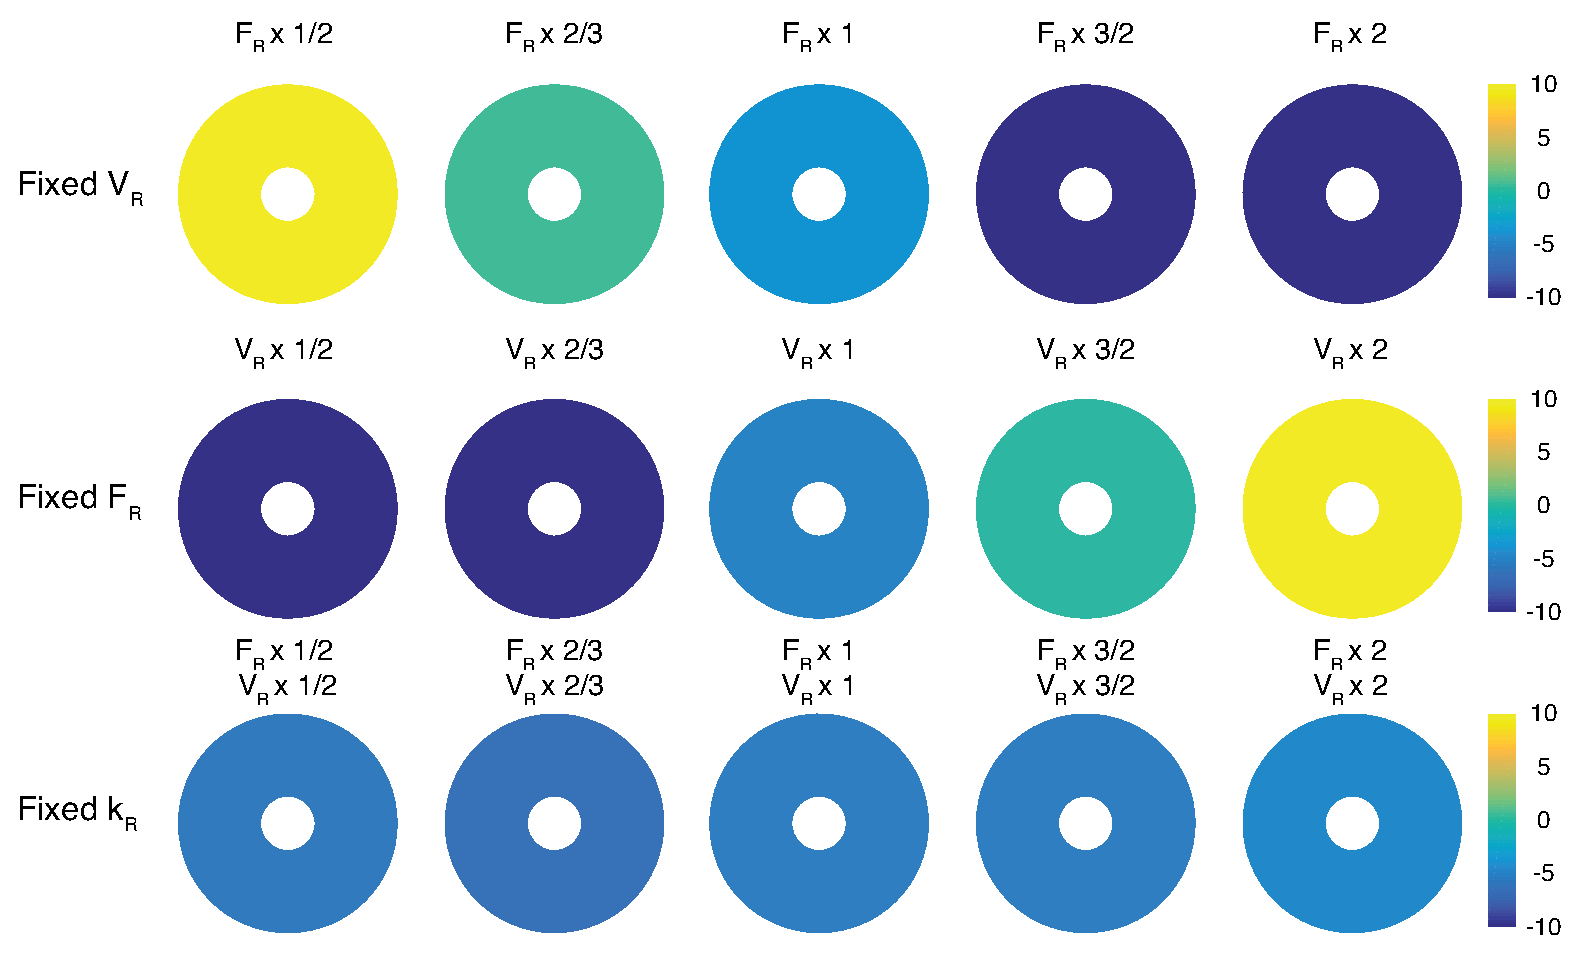
\includegraphics[width=\linewidth]{simRef_kR_rReg.eps}
        \caption{Bullseyes of the median relative estimation error for the rate constant in the reference tissue ($k_R$) estimated using the \textbf{rLin} (top) and \textbf{rReg} (bottom) models depending on the characteristics of the reference tissue used for simulation.}
        \label{fig:referenceTissue_kR}
    \end{figure}
\end{subfigures}
\FloatBarrier

\subsection{Number of regions}
The impact of varying the number of regions on the accuracy and precision of the estimates of the \textbf{rLin} and \textbf{rReg} models is shown in Figures~\ref{fig:region_rV} to \ref{fig:region_kR}.
Indeed, each figure corresponds to a parameter, and the first line represents the accuracy of the estimation through the median relative estimation error, while the second line represents the precision of the estimation through the standard deviation of the relative estimation error.
The relative tissue blood volume $rV$ (see Figure~\ref{fig:region_rV}) from the \textbf{rLin} and \textbf{rReg} models were slightly underestimated using both methods, the latter however yielded more homogeneous median biases across regions.
The \textbf{rLin} model was particularly imprecise in the region exhibiting the larger value of $k_T$.
For both models, no significant effect of the number of regions on the accuracy and precision of the estimates of $rV$ was observed in our simulations.
Using the \textbf{rLin} model, increasing the number of regions resulted in a lower precision of the regional estimates of $rF$, the relative tissue blood flow (see Figure~\ref{fig:region_rF}).
The \textbf{rReg} model yielded slightly more biased estimates of $rF$, but increasing the number of regions included in the analysis increased the precision of the estimation for studies including two or more regions.

Overall, the biases in the estimates of $rF$ from the \textbf{rReg} model were more consistent across tumor regions.
The rate constant in the tumor $k_T$ (see Figure~\ref{fig:region_kT}) was globally overestimated using the \textbf{rLin} model, except in the region with the largest simulated $k_T$ value where it was underestimated.
The most imprecise estimation of $k_T$ with this model were also found in the four regions exhibiting the largest simulated values of $k_T$.

Using the \textbf{rReg} model considerably reduced the median value of the estimation bias for studies including four or more regions, as well as its standard deviation for studies with eight or more regions.
Additionally, the estimation is more homogeneous across regions in terms of both accuracy and precision.
Regarding $k_R$, the rate constant in the reference tissue (see Figure~\ref{fig:region_kR}), the precision and the homogeneity of the estimates from the \textbf{rLin} model clearly decreases with the number of regions, while the precision actually increases using the \textbf{rReg} model. 
Increasing the number of regions increased the heterogeneity of the biases in the $k_R$ estimates of the \textbf{rLin} model.
The $k_R$ estimates of the \textbf{rReg} model exhibit a slight negative bias, which does not change much when changing the number of regions

\begin{subfigures}
    \begin{figure}\centering
        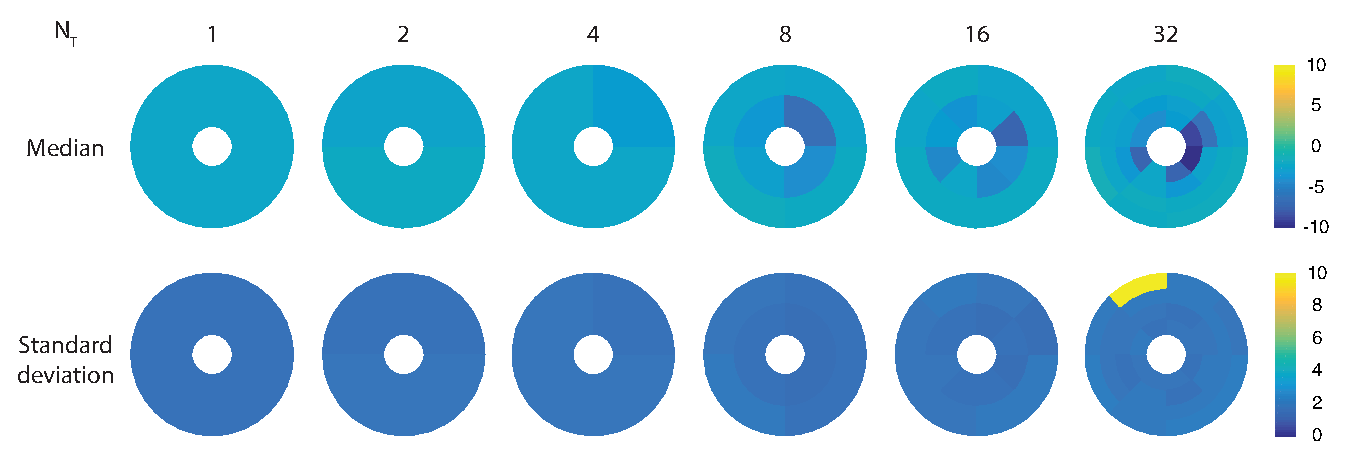
\includegraphics[width=0.9\linewidth]{simReg_rV_rLin.eps}
        \par%\vspace{1cm}
        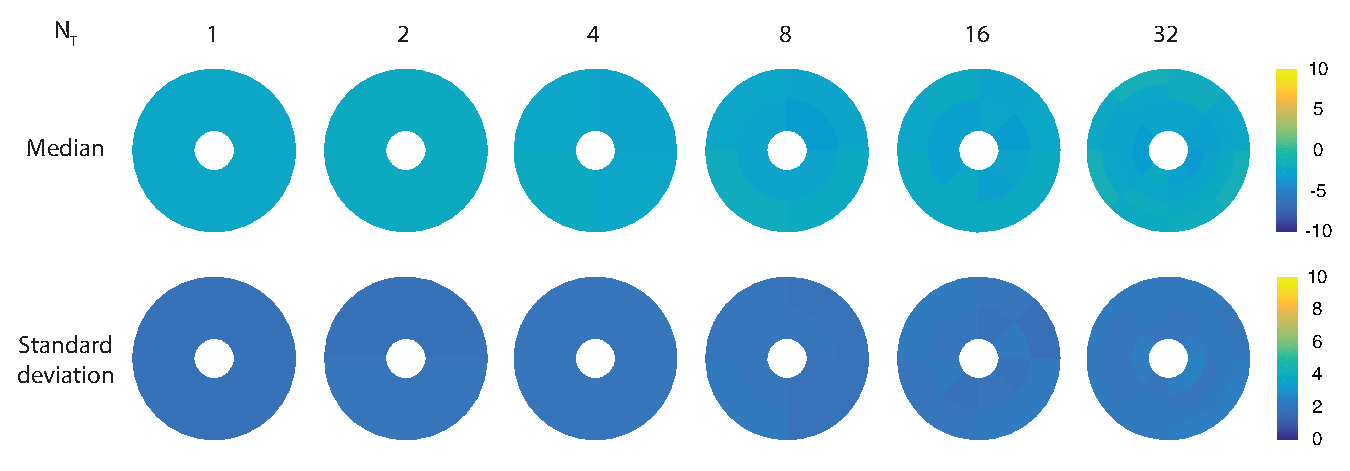
\includegraphics[width=0.9\linewidth]{simReg_rV_rReg.eps}
        \caption{Bullseyes of the median value and the standard deviation of the relative estimation error for the relative tissue blood volume ($rV$) estimated using the \textbf{rLin} (top) and \textbf{rReg} (bottom) models depending on the number of regions $N_T$.}
        \label{fig:region_rV}
    \end{figure}
    \begin{figure}\centering
        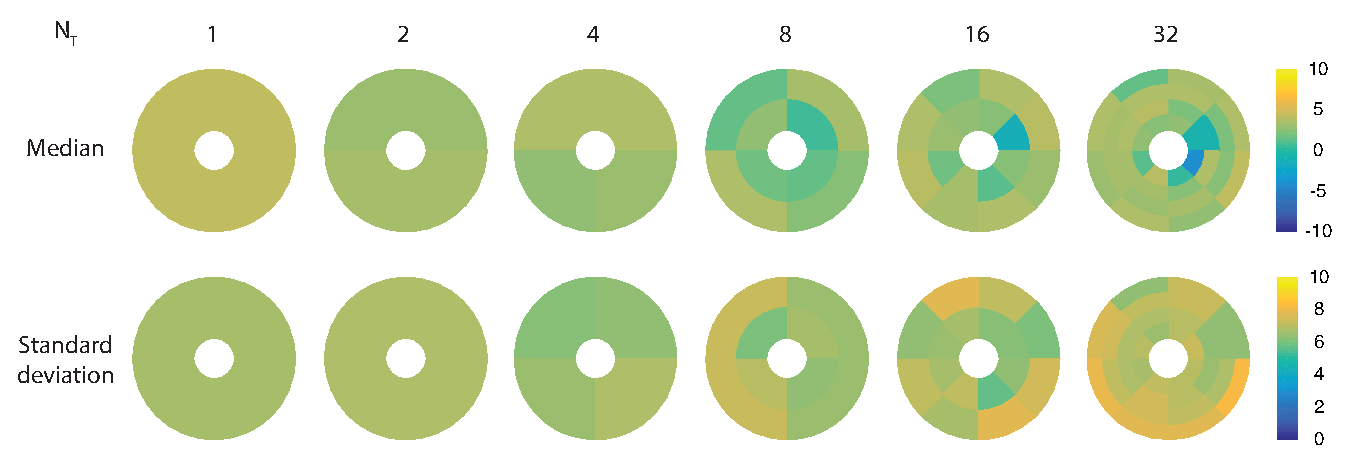
\includegraphics[width=0.9\linewidth]{simReg_rF_rLin.eps}
        \par%\vspace{1cm}
        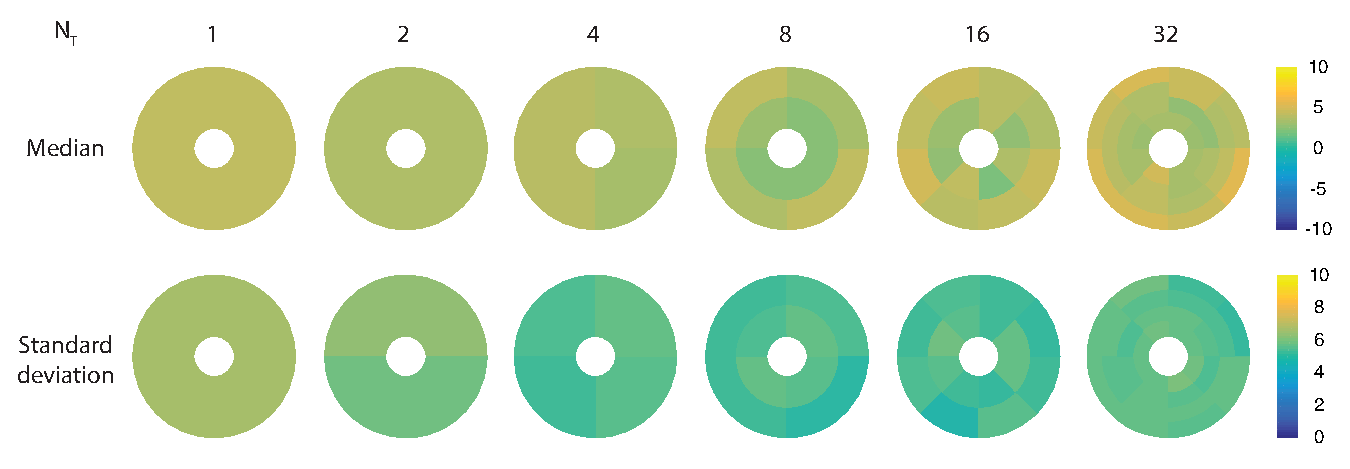
\includegraphics[width=0.9\linewidth]{simReg_rF_rReg.eps}
        \caption{Bullseyes of the median value and the standard deviation of the relative estimation error for the relative tissue blood volume ($rF$) estimated using the \textbf{rLin} (top) and \textbf{rReg} (bottom) models depending on the number of regions $N_T$.}
        \label{fig:region_rF}
    \end{figure}
    \begin{figure}\centering
        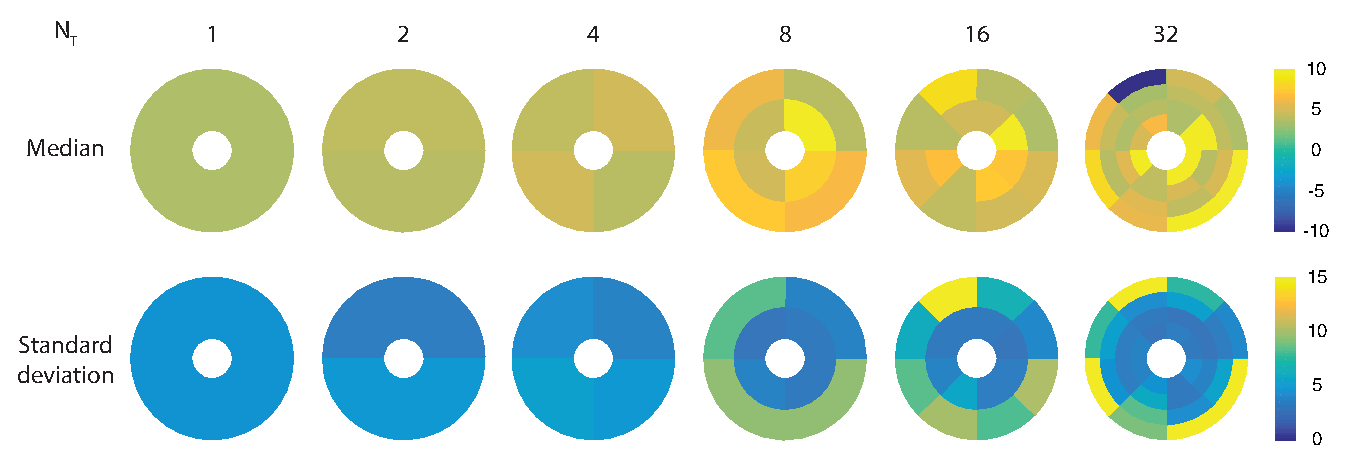
\includegraphics[width=0.9\linewidth]{simReg_kT_rLin.eps}
        \par%\vspace{1cm}
        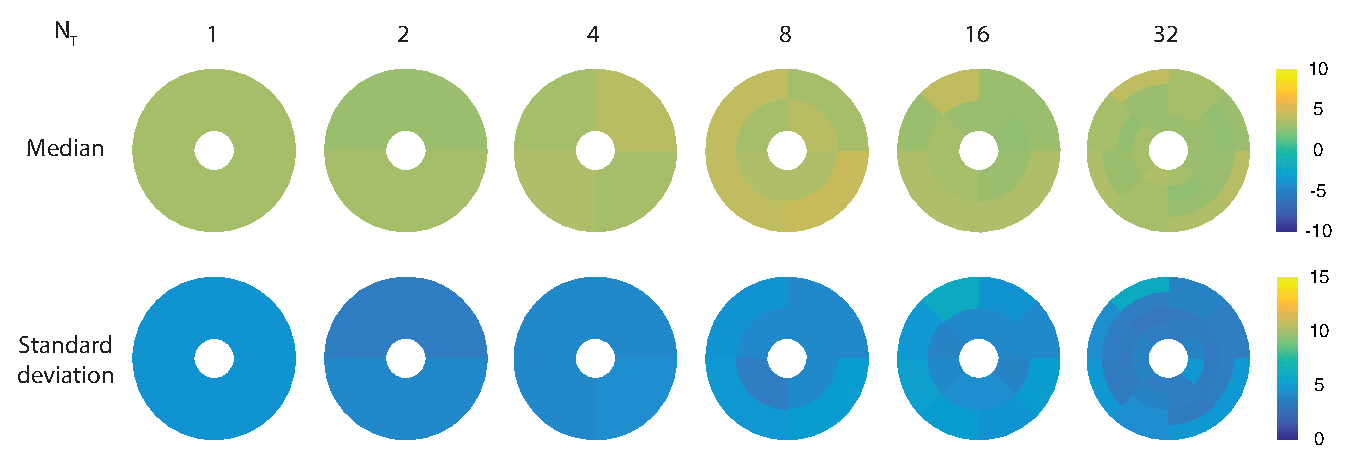
\includegraphics[width=0.9\linewidth]{simReg_kT_rReg.eps}
        \caption{Bullseyes of the median value and the standard deviation of the relative estimation error for the rate constant in the tumor ($k_T$) estimated using the \textbf{rLin} (top) and \textbf{rReg} (bottom) models depending on the number of regions $N_T$.}
        \label{fig:region_kT}
    \end{figure}
    \begin{figure}\centering
        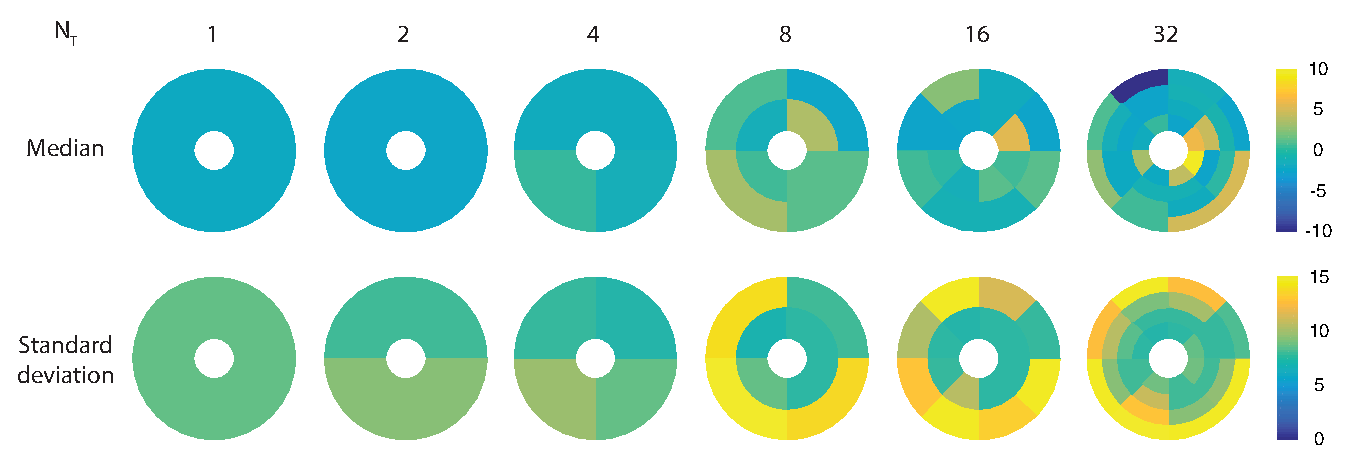
\includegraphics[width=0.9\linewidth]{simReg_kR_rLin.eps}
        \par%\vspace{1cm}
        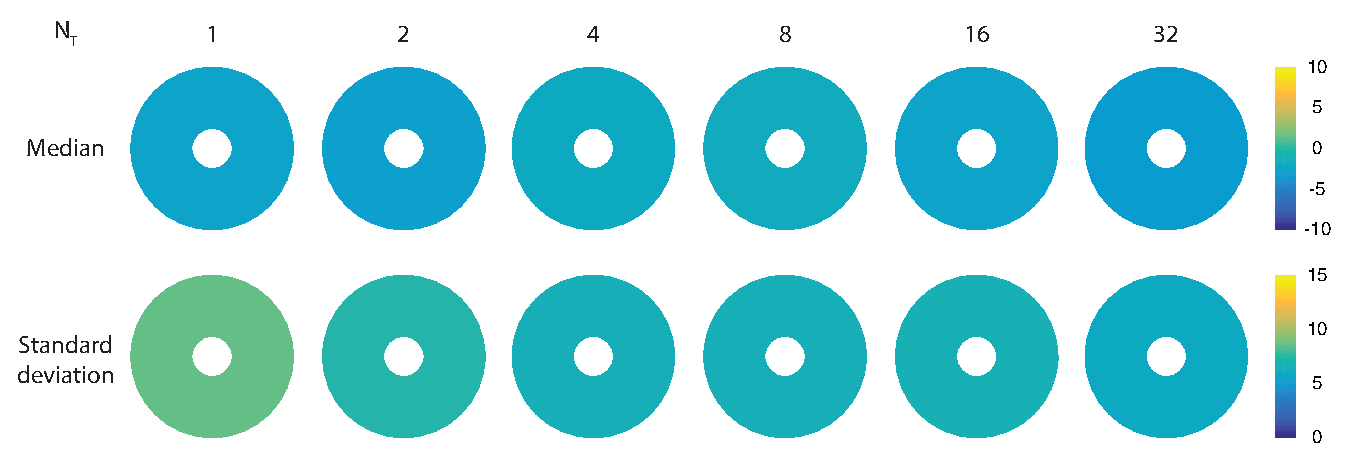
\includegraphics[width=0.9\linewidth]{simReg_kR_rReg.eps}
        \caption{Bullseyes of the median value and the standard deviation of the relative estimation error for the rate constant in the reference tissue ($k_R$) estimated using the \textbf{rLin} (top) and \textbf{rReg} (bottom) models depending on the number of regions $N_T$.}
        \label{fig:region_kR}
        \end{figure}
\end{subfigures}
\FloatBarrier

\section{Discussion}
In \citeyear{Logan:2001ip}, \citet{Logan:2001ip} investigated strategies to remove the bias in the graphical analysis of positron emission tomography data, which is basically a resolution method for the \textbf{OVC} model, i.e.~with a known arterial input function, but the study was also extended to the \textbf{rOVC} model, i.e.~with a reference tissue.
The linear formulation of the \textbf{rOVC} model, named \textbf{rLin} in this study, was assessed through simulation experiments with various noise levels, and various strategies were proposed to reduce the estimation bias of the distribution volume ratio, which is the generalization for the relative tissue blood volume when addressing non-intravascular tracers.
We first proposed the \textbf{rReg} model in \cite{Doury:2016fi} as a new strategy to improve parameter reproducibility in a test-retest preclinical study, and here we investigated the ability of the method to improve the homogeneity of the bias in the resolution of the \textbf{rOVC} model by taking advantage of the functional heterogeneity among the studied tissues.

The regularization greatly improved the homogeneity of the estimation across regions.
In some cases the regularization actually induced stronger bias in the estimation, however the biases are more homogeneous across regions, allowing meaningful regional comparison of the perfusion parameters.
Moreover, the \textbf{rLin} approach was largely outperformed by the \textbf{rReg}, especially regarding the accuracy of the rate constant estimates, $k_T$ and $k_R$, but also regarding the relative tissue blood volume and flow parameters, $rV$ and $rF$.
The regularization also made the estimation more robust to the acquisition settings over the investigated range, studied via the exam duration and the sampling period.

Theoretically, the number of regions included in the analysis should not have any impact on the parameters of the \textbf{rLin} model as every regional enhancement curve is modeled individually. 
In practice, increasing the number of regions and the underlying heterogeneity resulted in a large variability of the bias across regions.
Varying the number of regions reveals the importance of regularizing parameter $k_R$ across tumor regions, as implemented by the \textbf{rReg} model, by comparison with the \textbf{rLin} model.
The impact or regularization is measurable not only on $k_R$, but also on the other parameters.
In this study, simulations did not account for the variations of the signal to noise ratio depending on the size of the region.
Instead it investigates solely the impact of the number of regions included in the analysis on the accuracy and precision of the estimates depending on whether the approach is regularized for parameter $k_R$ by keeping the noise level constant regardless of the number of regions.

The rate constant in the tumor, $k_T$, appears to be related to the bias in the estimation of perfusion parameters using both models.
In particular for the \textbf{rReg} model, the region with a simulated $k_T$ value larger than $k_R$, and more generally regions with large $k_T$ values, yielded estimates of $k_T$ more biased than the other regions.
This phenomenon was reported by \citet{CardenasRodriguez:2013em} in a simulation study assessing the ability of the \textbf{rLin} model to accurately quantify perfusion in contrast-enhanced magnetic resonance imaging data.
The authors of this study applied the \textbf{rLin} model pixel by pixel, overlooking the relations between the local perfusion parameters.
However, regions with large $k_T$ values yielded accurate estimates of $rV$, while regions with small $k_T$ values yielded more biased estimates of the parameter.
Our experiments also reveal that estimation biases can either be positive or negative in a given region, depending on the value of $k_R$.

Our study revealed that the choice of the reference tissue plays a crucial role in the accuracy and precision of the perfusion parameters estimated using the \textbf{rReg} model, it should therefore be further investigated.
Indeed, it is necessary to identify the ideal reference tissue in order to improve the robustness of the estimation.
A deeper and finer understanding of the relations between the characteristics of the reference tissue and the estimated perfusion parameters may allow correction of the estimation bias in case the ideal reference tissue does not exist in the image.
Our study reveals that halving $V_R$ or doubling $F_R$, which both result in doubling $k_R$, has almost the same impact on the estimation bias.
Actually, the least biased estimation overall was obtained using two thirds of the original $k_R$ value, i.e.~$k_R = \frac{2}{3} \times 0.0693 = 0.0462$.
Additionally, increasing the values of both $V_R$ and $F_R$, while enforcing fixed values of $k_R$, increased the accuracy of the estimates of the \textbf{rReg} model.
This suggests that a well perfused tissue should be prefered, i.e.~a tissue with a high tissue blood flow and high tissue blood volume.

Different simulation studies should be conducted to investigate the applicability of the \textbf{rReg} models to contrast-enhanced images acquired using other imaging modalities in case of intravascular tracers, or in permeability-limited and flow-limited conditions with diffusing tracers, i.e.~when permeability or blood flow is much larger than the other one~\cite{Tofts:1999ih}, or when the data only reflects one of the processes~\cite{Balvay:2005ca}. 
Indeed, the range of investigated parameters should be adapted to the imaging modality of interest, for instance the sampling period and the exam duration are usually longer in other modalities than in ultrasound.
Additionally, the multiplicative noise model used for simulation is specific of ultrasound data, and the data was simulated using the \textbf{OVC} model to reflect the intravascular characteristics of ultrasound contrast agents. 


\section{Conclusion}
A simulation study based on preclinical contrast-enhanced ultrasound experiments was conducted to assess and compare the accuracy and precision of two estimation methods for the \textbf{rOVC} model, a one-compartment model using a reference tissue.
The \textbf{rLin} model relies on the linear formulation of the \textbf{rOVC} model, and estimates perfusion parameters in each region of analysis individually.
A limitation of this approach lies in the existence of a perfusion parameter that characterizes the unique reference tissue differently for each tumor region, i.e.~the rate constant $k_R$.
However, since the same reference tissue is used to analyse all the regions, this parameter should be homogeneous across the different regions.
The \textbf{rReg} model is based on the \textbf{rLin} model, but it takes advantage of the functional diversity of the regions under analysis, and ensures that the rate constant of the reference tissue is the same across all the regions.

These simulation studies demonstrated the superiority of the \textbf{rReg} model in terms of accuracy and precision.
The regularization of $k_R$ also made the biases more homogeneouse across regions, making comparison of regional parameters more meaningful.
Additionally, the \textbf{rReg} model relaxes the requirements for temporal resolution and exam duration, allowing accurate estimation of perfusion parameters in shorter acquisitions with low temporal resolution.
Our experiments suggest that the regularization improve the accuracy and precision of the estimation if at least four regions are included in the analysis.
Regarding the number and the size of the regions under analysis, a compromise should be made to reveal the spatial heterogeneity of the tissue, while limiting the noise level to ensure accurate estimation of the perfusion parameters.

Indeed the choice of the reference tissue is crucial as it has a significant impact on the accuracy of the estimation, and should be further investigated.
We were however able to draw some recommendations regarding its selection.
The rate constant parameter is critical when selecting the reference tissue, a region exhibiting a rate constant larger than the rate constants in the regions of analysis yielded more accurate parameters in our experiments.
Hhowever an optimal value of $k_R$ seems to exist, and this issue needs to be further investigated on real examples.
Furthermore, using a well perfused reference tissue, i.e.~a tissue with high tissue blood volume and tissue blood flow, appears to provide more accurate perfusion parameters.